\documentclass[nohyperref]{article}

\usepackage{etoolbox}
\newtoggle{arxiv}
\toggletrue{arxiv}

\usepackage{microtype}
\usepackage{graphicx}
\usepackage{subfigure}
\usepackage{booktabs} %
\usepackage{tabularx}
\usepackage{hyperref}
\usepackage{multirow}
\usepackage{setspace}
\usepackage{xfrac}
\newcommand{\theHalgorithm}{\arabic{algorithm}}

\iftoggle{arxiv}{
  \usepackage[numbers]{natbib}
}
{
\usepackage{icml2022}
}


\usepackage{amsmath}
\usepackage{amssymb}
\usepackage{mathtools}
\usepackage{amsthm}
\usepackage{relsize}
\usepackage{comment}
\usepackage{algorithm}
\usepackage{algorithmic}

\usepackage{subfigure}

\usepackage[capitalize]{cleveref}

\usepackage[inline]{enumitem}


\usepackage[textsize=tiny]{todonotes}

%%%%% NEW MATH DEFINITIONS %%%%%

\usepackage{amsmath,amsfonts,bm}

% Mark sections of captions for referring to divisions of figures
\newcommand{\figleft}{{\em (Left)}}
\newcommand{\figcenter}{{\em (Center)}}
\newcommand{\figright}{{\em (Right)}}
\newcommand{\figtop}{{\em (Top)}}
\newcommand{\figbottom}{{\em (Bottom)}}
\newcommand{\captiona}{{\em (a)}}
\newcommand{\captionb}{{\em (b)}}
\newcommand{\captionc}{{\em (c)}}
\newcommand{\captiond}{{\em (d)}}

% Highlight a newly defined term
\newcommand{\newterm}[1]{{\bf #1}}


% Figure reference, lower-case.
\def\figref#1{figure~\ref{#1}}
% Figure reference, capital. For start of sentence
\def\Figref#1{Figure~\ref{#1}}
\def\twofigref#1#2{figures \ref{#1} and \ref{#2}}
\def\quadfigref#1#2#3#4{figures \ref{#1}, \ref{#2}, \ref{#3} and \ref{#4}}
% Section reference, lower-case.
\def\secref#1{section~\ref{#1}}
% Section reference, capital.
\def\Secref#1{Section~\ref{#1}}
% Reference to two sections.
\def\twosecrefs#1#2{sections \ref{#1} and \ref{#2}}
% Reference to three sections.
\def\secrefs#1#2#3{sections \ref{#1}, \ref{#2} and \ref{#3}}
% Reference to an equation, lower-case.
% \def\eqref#1{equation~\ref{#1}}
\def\eqref#1{(\ref{#1})}
% Reference to an equation, upper case
\def\Eqref#1{Equation~\ref{#1}}
% A raw reference to an equation---avoid using if possible
\def\plaineqref#1{\ref{#1}}
% Reference to a chapter, lower-case.
\def\chapref#1{chapter~\ref{#1}}
% Reference to an equation, upper case.
\def\Chapref#1{Chapter~\ref{#1}}
% Reference to a range of chapters
\def\rangechapref#1#2{chapters\ref{#1}--\ref{#2}}
% Reference to an algorithm, lower-case.
\def\algref#1{algorithm~\ref{#1}}
% Reference to an algorithm, upper case.
\def\Algref#1{Algorithm~\ref{#1}}
\def\twoalgref#1#2{algorithms \ref{#1} and \ref{#2}}
\def\Twoalgref#1#2{Algorithms \ref{#1} and \ref{#2}}
% Reference to a part, lower case
\def\partref#1{part~\ref{#1}}
% Reference to a part, upper case
\def\Partref#1{Part~\ref{#1}}
\def\twopartref#1#2{parts \ref{#1} and \ref{#2}}

\def\ceil#1{\lceil #1 \rceil}
\def\floor#1{\lfloor #1 \rfloor}
\def\1{\bm{1}}
\newcommand{\train}{\mathcal{D}}
\newcommand{\valid}{\mathcal{D_{\mathrm{valid}}}}
\newcommand{\test}{\mathcal{D_{\mathrm{test}}}}

\def\eps{{\epsilon}}


% Random variables
\def\reta{{\textnormal{$\eta$}}}
\def\ra{{\textnormal{a}}}
\def\rb{{\textnormal{b}}}
\def\rc{{\textnormal{c}}}
\def\rd{{\textnormal{d}}}
\def\re{{\textnormal{e}}}
\def\rf{{\textnormal{f}}}
\def\rg{{\textnormal{g}}}
\def\rh{{\textnormal{h}}}
\def\ri{{\textnormal{i}}}
\def\rj{{\textnormal{j}}}
\def\rk{{\textnormal{k}}}
\def\rl{{\textnormal{l}}}
% rm is already a command, just don't name any random variables m
\def\rn{{\textnormal{n}}}
\def\ro{{\textnormal{o}}}
\def\rp{{\textnormal{p}}}
\def\rq{{\textnormal{q}}}
\def\rr{{\textnormal{r}}}
\def\rs{{\textnormal{s}}}
\def\rt{{\textnormal{t}}}
\def\ru{{\textnormal{u}}}
\def\rv{{\textnormal{v}}}
\def\rw{{\textnormal{w}}}
\def\rx{{\textnormal{x}}}
\def\ry{{\textnormal{y}}}
\def\rz{{\textnormal{z}}}

% Random vectors
\def\rvepsilon{{\mathbf{\epsilon}}}
\def\rvtheta{{\mathbf{\theta}}}
\def\rva{{\mathbf{a}}}
\def\rvb{{\mathbf{b}}}
\def\rvc{{\mathbf{c}}}
\def\rvd{{\mathbf{d}}}
\def\rve{{\mathbf{e}}}
\def\rvf{{\mathbf{f}}}
\def\rvg{{\mathbf{g}}}
\def\rvh{{\mathbf{h}}}
\def\rvu{{\mathbf{i}}}
\def\rvj{{\mathbf{j}}}
\def\rvk{{\mathbf{k}}}
\def\rvl{{\mathbf{l}}}
\def\rvm{{\mathbf{m}}}
\def\rvn{{\mathbf{n}}}
\def\rvo{{\mathbf{o}}}
\def\rvp{{\mathbf{p}}}
\def\rvq{{\mathbf{q}}}
\def\rvr{{\mathbf{r}}}
\def\rvs{{\mathbf{s}}}
\def\rvt{{\mathbf{t}}}
\def\rvu{{\mathbf{u}}}
\def\rvv{{\mathbf{v}}}
\def\rvw{{\mathbf{w}}}
\def\rvx{{\mathbf{x}}}
\def\rvy{{\mathbf{y}}}
\def\rvz{{\mathbf{z}}}

% Elements of random vectors
\def\erva{{\textnormal{a}}}
\def\ervb{{\textnormal{b}}}
\def\ervc{{\textnormal{c}}}
\def\ervd{{\textnormal{d}}}
\def\erve{{\textnormal{e}}}
\def\ervf{{\textnormal{f}}}
\def\ervg{{\textnormal{g}}}
\def\ervh{{\textnormal{h}}}
\def\ervi{{\textnormal{i}}}
\def\ervj{{\textnormal{j}}}
\def\ervk{{\textnormal{k}}}
\def\ervl{{\textnormal{l}}}
\def\ervm{{\textnormal{m}}}
\def\ervn{{\textnormal{n}}}
\def\ervo{{\textnormal{o}}}
\def\ervp{{\textnormal{p}}}
\def\ervq{{\textnormal{q}}}
\def\ervr{{\textnormal{r}}}
\def\ervs{{\textnormal{s}}}
\def\ervt{{\textnormal{t}}}
\def\ervu{{\textnormal{u}}}
\def\ervv{{\textnormal{v}}}
\def\ervw{{\textnormal{w}}}
\def\ervx{{\textnormal{x}}}
\def\ervy{{\textnormal{y}}}
\def\ervz{{\textnormal{z}}}

% Random matrices
\def\rmA{{\mathbf{A}}}
\def\rmB{{\mathbf{B}}}
\def\rmC{{\mathbf{C}}}
\def\rmD{{\mathbf{D}}}
\def\rmE{{\mathbf{E}}}
\def\rmF{{\mathbf{F}}}
\def\rmG{{\mathbf{G}}}
\def\rmH{{\mathbf{H}}}
\def\rmI{{\mathbf{I}}}
\def\rmJ{{\mathbf{J}}}
\def\rmK{{\mathbf{K}}}
\def\rmL{{\mathbf{L}}}
\def\rmM{{\mathbf{M}}}
\def\rmN{{\mathbf{N}}}
\def\rmO{{\mathbf{O}}}
\def\rmP{{\mathbf{P}}}
\def\rmQ{{\mathbf{Q}}}
\def\rmR{{\mathbf{R}}}
\def\rmS{{\mathbf{S}}}
\def\rmT{{\mathbf{T}}}
\def\rmU{{\mathbf{U}}}
\def\rmV{{\mathbf{V}}}
\def\rmW{{\mathbf{W}}}
\def\rmX{{\mathbf{X}}}
\def\rmY{{\mathbf{Y}}}
\def\rmZ{{\mathbf{Z}}}

% Elements of random matrices
\def\ermA{{\textnormal{A}}}
\def\ermB{{\textnormal{B}}}
\def\ermC{{\textnormal{C}}}
\def\ermD{{\textnormal{D}}}
\def\ermE{{\textnormal{E}}}
\def\ermF{{\textnormal{F}}}
\def\ermG{{\textnormal{G}}}
\def\ermH{{\textnormal{H}}}
\def\ermI{{\textnormal{I}}}
\def\ermJ{{\textnormal{J}}}
\def\ermK{{\textnormal{K}}}
\def\ermL{{\textnormal{L}}}
\def\ermM{{\textnormal{M}}}
\def\ermN{{\textnormal{N}}}
\def\ermO{{\textnormal{O}}}
\def\ermP{{\textnormal{P}}}
\def\ermQ{{\textnormal{Q}}}
\def\ermR{{\textnormal{R}}}
\def\ermS{{\textnormal{S}}}
\def\ermT{{\textnormal{T}}}
\def\ermU{{\textnormal{U}}}
\def\ermV{{\textnormal{V}}}
\def\ermW{{\textnormal{W}}}
\def\ermX{{\textnormal{X}}}
\def\ermY{{\textnormal{Y}}}
\def\ermZ{{\textnormal{Z}}}

% Vectors
\def\vzero{{\bm{0}}}
\def\vone{{\bm{1}}}
\def\vmu{{\bm{\mu}}}
\def\vtheta{{\bm{\theta}}}
\def\va{{\bm{a}}}
\def\vb{{\bm{b}}}
\def\vc{{\bm{c}}}
\def\vd{{\bm{d}}}
\def\ve{{\bm{e}}}
\def\vf{{\bm{f}}}
\def\vg{{\bm{g}}}
\def\vh{{\bm{h}}}
\def\vi{{\bm{i}}}
\def\vj{{\bm{j}}}
\def\vk{{\bm{k}}}
\def\vl{{\bm{l}}}
\def\vm{{\bm{m}}}
\def\vn{{\bm{n}}}
\def\vo{{\bm{o}}}
\def\vp{{\bm{p}}}
\def\vq{{\bm{q}}}
\def\vr{{\bm{r}}}
\def\vs{{\bm{s}}}
\def\vt{{\bm{t}}}
\def\vu{{\bm{u}}}
\def\vv{{\bm{v}}}
\def\vw{{\bm{w}}}
\def\vx{{\bm{x}}}
\def\vy{{\bm{y}}}
\def\vz{{\bm{z}}}

% Elements of vectors
\def\evalpha{{\alpha}}
\def\evbeta{{\beta}}
\def\evepsilon{{\epsilon}}
\def\evlambda{{\lambda}}
\def\evomega{{\omega}}
\def\evmu{{\mu}}
\def\evpsi{{\psi}}
\def\evsigma{{\sigma}}
\def\evtheta{{\theta}}
\def\eva{{a}}
\def\evb{{b}}
\def\evc{{c}}
\def\evd{{d}}
\def\eve{{e}}
\def\evf{{f}}
\def\evg{{g}}
\def\evh{{h}}
\def\evi{{i}}
\def\evj{{j}}
\def\evk{{k}}
\def\evl{{l}}
\def\evm{{m}}
\def\evn{{n}}
\def\evo{{o}}
\def\evp{{p}}
\def\evq{{q}}
\def\evr{{r}}
\def\evs{{s}}
\def\evt{{t}}
\def\evu{{u}}
\def\evv{{v}}
\def\evw{{w}}
\def\evx{{x}}
\def\evy{{y}}
\def\evz{{z}}

% Matrix
\def\mA{{\bm{A}}}
\def\mB{{\bm{B}}}
\def\mC{{\bm{C}}}
\def\mD{{\bm{D}}}
\def\mE{{\bm{E}}}
\def\mF{{\bm{F}}}
\def\mG{{\bm{G}}}
\def\mH{{\bm{H}}}
\def\mI{{\bm{I}}}
\def\mJ{{\bm{J}}}
\def\mK{{\bm{K}}}
\def\mL{{\bm{L}}}
\def\mM{{\bm{M}}}
\def\mN{{\bm{N}}}
\def\mO{{\bm{O}}}
\def\mP{{\bm{P}}}
\def\mQ{{\bm{Q}}}
\def\mR{{\bm{R}}}
\def\mS{{\bm{S}}}
\def\mT{{\bm{T}}}
\def\mU{{\bm{U}}}
\def\mV{{\bm{V}}}
\def\mW{{\bm{W}}}
\def\mX{{\bm{X}}}
\def\mY{{\bm{Y}}}
\def\mZ{{\bm{Z}}}
\def\mBeta{{\bm{\beta}}}
\def\mPhi{{\bm{\Phi}}}
\def\mLambda{{\bm{\Lambda}}}
\def\mSigma{{\bm{\Sigma}}}

% Tensor
\DeclareMathAlphabet{\mathsfit}{\encodingdefault}{\sfdefault}{m}{sl}
\SetMathAlphabet{\mathsfit}{bold}{\encodingdefault}{\sfdefault}{bx}{n}
\newcommand{\tens}[1]{\bm{\mathsfit{#1}}}
\def\tA{{\tens{A}}}
\def\tB{{\tens{B}}}
\def\tC{{\tens{C}}}
\def\tD{{\tens{D}}}
\def\tE{{\tens{E}}}
\def\tF{{\tens{F}}}
\def\tG{{\tens{G}}}
\def\tH{{\tens{H}}}
\def\tI{{\tens{I}}}
\def\tJ{{\tens{J}}}
\def\tK{{\tens{K}}}
\def\tL{{\tens{L}}}
\def\tM{{\tens{M}}}
\def\tN{{\tens{N}}}
\def\tO{{\tens{O}}}
\def\tP{{\tens{P}}}
\def\tQ{{\tens{Q}}}
\def\tR{{\tens{R}}}
\def\tS{{\tens{S}}}
\def\tT{{\tens{T}}}
\def\tU{{\tens{U}}}
\def\tV{{\tens{V}}}
\def\tW{{\tens{W}}}
\def\tX{{\tens{X}}}
\def\tY{{\tens{Y}}}
\def\tZ{{\tens{Z}}}


% Graph
\def\gA{{\mathcal{A}}}
\def\gB{{\mathcal{B}}}
\def\gC{{\mathcal{C}}}
\def\gD{{\mathcal{D}}}
\def\gE{{\mathcal{E}}}
\def\gF{{\mathcal{F}}}
\def\gG{{\mathcal{G}}}
\def\gH{{\mathcal{H}}}
\def\gI{{\mathcal{I}}}
\def\gJ{{\mathcal{J}}}
\def\gK{{\mathcal{K}}}
\def\gL{{\mathcal{L}}}
\def\gM{{\mathcal{M}}}
\def\gN{{\mathcal{N}}}
\def\gO{{\mathcal{O}}}
\def\gP{{\mathcal{P}}}
\def\gQ{{\mathcal{Q}}}
\def\gR{{\mathcal{R}}}
\def\gS{{\mathcal{S}}}
\def\gT{{\mathcal{T}}}
\def\gU{{\mathcal{U}}}
\def\gV{{\mathcal{V}}}
\def\gW{{\mathcal{W}}}
\def\gX{{\mathcal{X}}}
\def\gY{{\mathcal{Y}}}
\def\gZ{{\mathcal{Z}}}

% Sets
\def\sA{{\mathbb{A}}}
\def\sB{{\mathbb{B}}}
\def\sC{{\mathbb{C}}}
\def\sD{{\mathbb{D}}}
% Don't use a set called E, because this would be the same as our symbol
% for expectation.
\def\sF{{\mathbb{F}}}
\def\sG{{\mathbb{G}}}
\def\sH{{\mathbb{H}}}
\def\sI{{\mathbb{I}}}
\def\sJ{{\mathbb{J}}}
\def\sK{{\mathbb{K}}}
\def\sL{{\mathbb{L}}}
\def\sM{{\mathbb{M}}}
\def\sN{{\mathbb{N}}}
\def\sO{{\mathbb{O}}}
\def\sP{{\mathbb{P}}}
\def\sQ{{\mathbb{Q}}}
\def\sR{{\mathbb{R}}}
\def\sS{{\mathbb{S}}}
\def\sT{{\mathbb{T}}}
\def\sU{{\mathbb{U}}}
\def\sV{{\mathbb{V}}}
\def\sW{{\mathbb{W}}}
\def\sX{{\mathbb{X}}}
\def\sY{{\mathbb{Y}}}
\def\sZ{{\mathbb{Z}}}

% Entries of a matrix
\def\emLambda{{\Lambda}}
\def\emA{{A}}
\def\emB{{B}}
\def\emC{{C}}
\def\emD{{D}}
\def\emE{{E}}
\def\emF{{F}}
\def\emG{{G}}
\def\emH{{H}}
\def\emI{{I}}
\def\emJ{{J}}
\def\emK{{K}}
\def\emL{{L}}
\def\emM{{M}}
\def\emN{{N}}
\def\emO{{O}}
\def\emP{{P}}
\def\emQ{{Q}}
\def\emR{{R}}
\def\emS{{S}}
\def\emT{{T}}
\def\emU{{U}}
\def\emV{{V}}
\def\emW{{W}}
\def\emX{{X}}
\def\emY{{Y}}
\def\emZ{{Z}}
\def\emSigma{{\Sigma}}

% entries of a tensor
% Same font as tensor, without \bm wrapper
\newcommand{\etens}[1]{\mathsfit{#1}}
\def\etLambda{{\etens{\Lambda}}}
\def\etA{{\etens{A}}}
\def\etB{{\etens{B}}}
\def\etC{{\etens{C}}}
\def\etD{{\etens{D}}}
\def\etE{{\etens{E}}}
\def\etF{{\etens{F}}}
\def\etG{{\etens{G}}}
\def\etH{{\etens{H}}}
\def\etI{{\etens{I}}}
\def\etJ{{\etens{J}}}
\def\etK{{\etens{K}}}
\def\etL{{\etens{L}}}
\def\etM{{\etens{M}}}
\def\etN{{\etens{N}}}
\def\etO{{\etens{O}}}
\def\etP{{\etens{P}}}
\def\etQ{{\etens{Q}}}
\def\etR{{\etens{R}}}
\def\etS{{\etens{S}}}
\def\etT{{\etens{T}}}
\def\etU{{\etens{U}}}
\def\etV{{\etens{V}}}
\def\etW{{\etens{W}}}
\def\etX{{\etens{X}}}
\def\etY{{\etens{Y}}}
\def\etZ{{\etens{Z}}}

% The true underlying data generating distribution
\newcommand{\pdata}{p_{\rm{data}}}
% The empirical distribution defined by the training set
\newcommand{\ptrain}{\hat{p}_{\rm{data}}}
\newcommand{\Ptrain}{\hat{P}_{\rm{data}}}
% The model distribution
\newcommand{\pmodel}{p_{\rm{model}}}
\newcommand{\Pmodel}{P_{\rm{model}}}
\newcommand{\ptildemodel}{\tilde{p}_{\rm{model}}}
% Stochastic autoencoder distributions
\newcommand{\pencode}{p_{\rm{encoder}}}
\newcommand{\pdecode}{p_{\rm{decoder}}}
\newcommand{\precons}{p_{\rm{reconstruct}}}

\newcommand{\laplace}{\mathrm{Laplace}} % Laplace distribution

\newcommand{\E}{\mathbb{E}}
\newcommand{\Ls}{\mathcal{L}}
\newcommand{\R}{\mathbb{R}}
\newcommand{\emp}{\tilde{p}}
\newcommand{\lr}{\alpha}
\newcommand{\reg}{\lambda}
\newcommand{\rect}{\mathrm{rectifier}}
\newcommand{\softmax}{\mathrm{softmax}}
\newcommand{\sigmoid}{\sigma}
\newcommand{\softplus}{\zeta}
\newcommand{\KL}{D_{\mathrm{KL}}}
\newcommand{\Var}{\mathrm{Var}}
\newcommand{\standarderror}{\mathrm{SE}}
\newcommand{\Cov}{\mathrm{Cov}}
% Wolfram Mathworld says $L^2$ is for function spaces and $\ell^2$ is for vectors
% But then they seem to use $L^2$ for vectors throughout the site, and so does
% wikipedia.
\newcommand{\normlzero}{L^0}
\newcommand{\normlone}{L^1}
\newcommand{\normltwo}{L^2}
\newcommand{\normlp}{L^p}
\newcommand{\normmax}{L^\infty}

\newcommand{\parents}{Pa} % See usage in notation.tex. Chosen to match Daphne's book.

\DeclareMathOperator*{\argmax}{arg\,max}
\DeclareMathOperator*{\argmin}{arg\,min}

\DeclareMathOperator{\sign}{sign}
\DeclareMathOperator{\Tr}{Tr}
\let\ab\allowbreak

\newtoggle{comment}
\toggletrue{comment}
\togglefalse{comment} %

\iftoggle{comment}{
\newcommand{\Beidi}[1]{{\color{orange} [Beidi: {#1}]}}
\newcommand{\Tri}[1]{{\color{cyan} [Tri: {#1}]}}
\newcommand{\nimit}[1]{{\color{red} [Nimit: {#1}]}}
\newcommand{\micp}[1]{{\color{blue!70} [Michael: {#1}]}}
\newcommand{\arjun}[1]{{\color{green} [Arjun: {#1}]}}
}{
\newcommand{\Beidi}[1]{}
\newcommand{\Tri}[1]{}
\newcommand{\nimit}[1]{}
\newcommand{\micp}[1]{}
\newcommand{\arjun}[1]{}
}

\iftoggle{arxiv}{
  \setlength{\textwidth}{6.5in}
  \setlength{\textheight}{9in}
  \setlength{\oddsidemargin}{0in}
  \setlength{\evensidemargin}{0in}
  \setlength{\topmargin}{-0.5in}
  \newlength{\defbaselineskip}
  \setlength{\defbaselineskip}{\baselineskip}
  \setlength{\marginparwidth}{0.8in}
}{
\usepackage[compact]{titlesec}
\titlespacing{\section}{0pt}{*1.0}{*0}
\titlespacing{\subsection}{0pt}{*0}{*0}
\titlespacing{\subsubsection}{0pt}{*0}{*0}

\usepackage[subtle, mathdisplays=tight, charwidths=tight, leading=normal]{savetrees}


\def\setstretch#1{\renewcommand{\baselinestretch}{#1}}
\setstretch{0.99}
\addtolength{\parskip}{-0.3pt}
}


\iftoggle{arxiv}{
\title{Monarch: Expressive Structured Matrices for Efficient and Accurate Training}
\usepackage{authblk}
\author[1]{Tri Dao}
\author[1]{Beidi Chen}
\author[1]{Nimit Sohoni}
\author[1]{Arjun Desai}
\author[1]{Michael Poli}
\author[2]{Jessica Grogan}
\author[3]{Alexander Liu}
\author[3]{Aniruddh Rao}
\author[2]{Atri Rudra}
\author[1]{Christopher R{\'e}}
\affil[1]{Stanford University}
\affil[2]{University at Buffalo, SUNY}
\affil[2]{University of Michigan}
\affil[ ]{\texttt{\{trid,beidic,nims,arjundd,poli\}@stanford.edu}, \texttt{\{jrgrogan,atri\}@buffalo.edu}, \texttt{\{avliu,anrao\}@umich.edu}, \texttt{chrismre@cs.stanford.edu}}
}{
\icmltitlerunning{Monarch}
}

\begin{document}


\iftoggle{arxiv}{
  \maketitle
}{
\twocolumn[
\icmltitle{Monarch: Expressive Structured Matrices for Efficient and Accurate Training}



\icmlsetsymbol{equal}{*}

\begin{icmlauthorlist}
\icmlauthor{Firstname1 Lastname1}{equal,yyy}
\icmlauthor{Firstname2 Lastname2}{equal,yyy,comp}
\icmlauthor{Firstname3 Lastname3}{comp}
\icmlauthor{Firstname4 Lastname4}{sch}
\icmlauthor{Firstname5 Lastname5}{yyy}
\icmlauthor{Firstname6 Lastname6}{sch,yyy,comp}
\icmlauthor{Firstname7 Lastname7}{comp}
\icmlauthor{Firstname8 Lastname8}{sch}
\icmlauthor{Firstname8 Lastname8}{yyy,comp}
\end{icmlauthorlist}

\icmlaffiliation{yyy}{Department of XXX, University of YYY, Location, Country}
\icmlaffiliation{comp}{Company Name, Location, Country}
\icmlaffiliation{sch}{School of ZZZ, Institute of WWW, Location, Country}

\icmlcorrespondingauthor{Firstname1 Lastname1}{first1.last1@xxx.edu}
\icmlcorrespondingauthor{Firstname2 Lastname2}{first2.last2@www.uk}

\icmlkeywords{Machine Learning, ICML}

\vskip 0.3in
]



\printAffiliationsAndNotice{\icmlEqualContribution} %
}

\begin{abstract}
  Large neural networks excel in many domains, but they are expensive to train and fine-tune.
  A popular approach to reduce their compute/memory requirements is to replace dense weight matrices with structured ones (e.g., sparse, low-rank, Fourier transform).
  These methods have not seen widespread adoption (1) in end-to-end training due to
  unfavorable efficiency--quality tradeoffs, and
  (2) in dense-to-sparse fine-tuning due to lack of tractable algorithms to
  approximate a given dense weight matrix.
  To address these issues, we propose a class of matrices (Monarch) that is \emph{hardware-efficient} (they are parameterized as products of two block-diagonal matrices for better hardware utilization) and \emph{expressive} (they can represent many commonly used transforms).
  Surprisingly, the problem of approximating a dense weight matrix with a Monarch matrix, though nonconvex, has an analytical optimal solution.
  These properties of Monarch matrices unlock new ways to train and fine-tune sparse and dense models.
  We empirically validate that Monarch can achieve favorable accuracy–efficiency tradeoffs in several end-to-end sparse training applications: speeding up ViT and GPT-2 training on ImageNet classification and Wikitext-103 language modeling by 2$\times$ with comparable model quality, and reducing the error on PDE solving and MRI reconstruction tasks by 40\%.
  In sparse-to-dense training, with a simple technique called ``reverse sparsification,'' Monarch matrices serve as a useful intermediate representation to speed up GPT-2 pretraining on OpenWebText by 2$\times$ without quality drop.
  The same technique brings 23\% faster BERT pretraining than even the very optimized implementation from Nvidia that set the MLPerf 1.1 record.
  In dense-to-sparse fine-tuning, as a proof-of-concept, our Monarch approximation algorithm speeds up BERT fine-tuning on GLUE by 1.7$\times$ with comparable accuracy.
\end{abstract}

\documentclass[11pt]{report}
\usepackage[margin=2cm]{geometry}
\usepackage{graphicx}
\usepackage{float}
\usepackage{times}
\usepackage{url}
\usepackage[dvipsnames]{xcolor}
\usepackage{hyperref}

\newcommand{\specialcell}[2][c]{\begin{tabular}[#1]{@{}c@{}}#2\end{tabular}}

\newcommand{\Gap}{\texorpdfstring{\hfill}{}}
\newcommand{\Rec}{\texorpdfstring{{\small\emph{\color{ccai-blue}{\fbox{High Leverage}}}}}{}}
\newcommand{\HighRisk}{\texorpdfstring{{\small\emph{\color{ccai-yellow-darker}{\fbox{Uncertain Impact}}}}}{}}
\newcommand{\Longterm}{\texorpdfstring{{\small\emph{\color{ccai-green}{\fbox{Long-term}}}}}{}}

\begin{document}

\begin{abstract}
Climate change is one of the greatest challenges facing humanity, and we, as machine learning experts, may wonder how we can help. Here we describe how machine learning can be a powerful tool in reducing greenhouse gas emissions and helping society adapt to a changing climate. From smart grids to disaster management, we identify high impact problems where existing gaps can be filled by machine learning, in collaboration with other fields. Our recommendations encompass exciting research questions as well as promising business opportunities. We call on the machine learning community to join the global effort against climate change.
\vskip .5in
\end{abstract}

\part*{Introduction}
The effects of climate change are increasingly visible.\footnote{For a layman's introduction to the topic of climate change, see \cite{romm2018climate, archer2010climate}.} Storms, droughts, fires, and flooding have become stronger and more frequent \cite{field2012managing}. Global ecosystems are changing, including the natural resources and agriculture on which humanity depends. The 2018 intergovernmental report on climate change estimated that the world will face catastrophic consequences unless global greenhouse gas emissions are eliminated within thirty years \cite{ipcc_global_2018}. Yet year after year, these emissions rise.

Addressing climate change involves mitigation (reducing emissions) and adaptation (preparing for unavoidable consequences). Both are multifaceted issues. Mitigation of greenhouse gas (GHG) emissions requires changes to electricity systems, transportation, buildings, industry, and land use. Adaptation requires planning for resilience and disaster management, given an understanding of climate and extreme events. Such a diversity of problems can be seen as an opportunity: there are many ways to have an impact.

In recent years, machine learning (ML) has been recognized as a broadly powerful tool for technological progress. Despite the growth of movements applying ML and AI to problems of societal and global good,\footnote{See the AI for social good movement (e.g.~\cite{hager2019artificial, berendt2019ai}), ML for the developing world~\cite{de2018machine}, the computational sustainability movement (e.g.~\cite{kelling2018computational, joppa2017case, lassig2016computational, gomes2009computational, dietterich2009machine}, the American Meteorological Society's Committee on AI Applications to Environmental Science, and the field of Climate Informatics (\url{www.climateinformatics.org}) \cite{Monteleoni2013chapter}, as well as the relevant survey papers \cite{faghmous2014big, kaack2019challenges, ford2016opinion}.} there remains the need for a concerted effort to identify how these tools may best be applied to tackle climate change. Many ML practitioners wish to act, but are uncertain how. On the other side, many fields have begun actively seeking input from the ML community.

This paper aims to provide an overview of where machine learning can be applied with high impact in the fight against climate change, through either effective engineering or innovative research. The strategies we highlight include climate mitigation and adaptation, as well as meta-level tools that enable other strategies. In order to maximize the relevance of our recommendations, we have consulted experts across many fields (see \hyperref[sec:acknowledgments]{{\small{Acknowledgments}}}) in the preparation of this paper.


\begin{table}
\begin{small}
\begin{center}
\begin{tabular}{l l l l l l l l l l l l}  \toprule
     \multicolumn{2}{l}{ }
         & \small{\rotatebox{90}{\parbox{2.2cm}{Causal\\inference}}}
         & \small{\rotatebox{90}{\parbox{2.2cm}{Computer\\vision}}}
         & \small{\rotatebox{90}{\parbox{2.2cm}{Interpretable\\models}}}
         & \small{\rotatebox{90}{NLP}}
         & \small{\rotatebox{90}{\parbox{2.2cm}{RL \& Control}}}
        %  & \small{\rotatebox{90}{Robotics}}
         & \small{\rotatebox{90}{\parbox{2.2cm}{Time-series analysis}}}
         & \small{\rotatebox{90}{\parbox{2.2cm}{Transfer\\learning}}}
         & \small{\rotatebox{90}{\parbox{2.2cm}{Uncertainty\\quantification}}}
         & \small{\rotatebox{90}{\parbox{2.2cm}{Unsupervised\\learning}}}
    \\ \midrule
    \rowcolor{ccai-blue-lightest}
    \multicolumn{2}{l}{1 \hyperref[sec:electricity-systems]{Electricity systems}} 
        & % Causal inf
        &  % Comp vision
        & % Interpretable ml
        & % nlp
        & % rl + control
        & % time series
        & % transfer
        & % UQ
        & \\% unsupervised \ref{sub
    & \hyperref[sec:electricity-lowCarbon]{Enabling low-carbon electricity}
        & % Causal inf
        & $\bullet$% Comp vision
        & $\bullet$% % Interpretable ml
        & % % nlp
        & $\bullet$%% rl + control
        & $\bullet$% % time series
        & % transfer
        & $\bullet$% % UQ
        & $\bullet$\\% unsupervised 
    & \hyperref[sec:electricity-currentSystemImpact]{Reducing current-system impacts}
        & % Causal inf
        & $\bullet$% Comp vision
        & % Interpretable ml
        & % nlp
        & % rl + control
        & $\bullet$% % time series
        & % transfer
        & $\bullet$% % UQ
        & $\bullet$\\% unsupervised 
    & \hyperref[sec:electricity-developing]{Ensuring global impact}
        & % Causal inf
        & $\bullet$% Comp vision
        & % Interpretable ml
        & % nlp
        & % rl + control
        & % time series
        & $\bullet$ % transfer
        & % UQ
        & $\bullet$\\% unsupervised 
    \rowcolor{ccai-blue-lightest}
    \multicolumn{2}{l}{2 \hyperref[sec:transportation]{Transportation}} 
        & % Causal inf
        & % Comp vision
        &% Interpretable ml
        & % nlp
        & % rl + control
        & % time series
        & % transfer
        & % UQ
        & \\% unsupervised 
    & \hyperref[sec:TReducing]{Reducing transport activity}
        & % Causal inf
        & $\bullet$% Comp vision
        & % Interpretable ml
        & % nlp
        & % rl + control
        & $\bullet$% time series
        & % transfer
        & $\bullet$% UQ
        & $\bullet$\\% unsupervised     
   & \hyperref[sec:TEfficient]{Improving vehicle efficiency}
        & % Causal inf
        & $\bullet$% Comp vision
        & % Interpretable ml
        & % nlp
        & $\bullet$% rl + control
        & % time series
        & % transfer
        & % UQ
        & \\% unsupervised    
   & \hyperref[sec:TFuels]{Alternative fuels \& electrification}
        & % Causal inf
        & % Comp vision
        & % Interpretable ml
        & % nlp
        & $\bullet$% rl + control
        & % time series
        & % transfer
        & % UQ
        & $\bullet$ \\% unsupervised    
   & \hyperref[sec:modalshift]{Modal shift}
        & $\bullet$% Causal inf
        & $\bullet$% Comp vision
        & % Interpretable ml
        & % nlp
        & % rl + control
        & $\bullet$% time series
        & % transfer
        & $\bullet$% UQ
        & \\% unsupervised    
    \rowcolor{ccai-blue-lightest}
    \multicolumn{2}{l}{3 \hyperref[sec:buildings-cities]{Buildings and cities}} 
        & % Causal inf
        & % Comp vision
        & % Interpretable ml
        & % nlp
        & % rl + control
        & % time series
        & % transfer
        & % UQ
        & \\% unsupervised 
    & \hyperref[sec:indv]{Optimizing buildings}
        & $\bullet$% Causal inf
        & % Comp vision
        & % Interpretable ml
        & % nlp
        & $\bullet$% rl + control
        & $\bullet$% time series
        & $\bullet$% transfer
        & % UQ
        & \\% unsupervised 
    & \hyperref[sec:distr]{Urban planning}
        & % Causal inf
        & $\bullet$% Comp vision
        & % Interpretable ml
        & % nlp
        & % rl + control
        & $\bullet$% time series
        & $\bullet$% transfer
        & % UQ
        & $\bullet$\\% unsupervised 
    & \hyperref[sec:cities]{The future of cities}
        & % Causal inf
        & % Comp vision
        & % Interpretable ml
        & $\bullet$%% nlp
        & % rl + control
        & %% time series
        & $\bullet$%% transfer
        & $\bullet$% UQ
        & $\bullet$\\% unsupervised 
    \rowcolor{ccai-blue-lightest}
    \multicolumn{2}{l}{4 \hyperref[sec:industry]{Industry}} 
        & % Causal inf
        & % Comp vision
        & % Interpretable ml
        & % nlp
        & % rl + control
        & % time series
        & % transfer
        & % UQ
        & \\% unsupervised 
    & \hyperref[sec:supplychains]{Optimizing supply chains}
        & % Causal inf
        & $\bullet$ %% Comp vision
        & % Interpretable ml
        & % nlp
        & $\bullet$ % rl + control
        & $\bullet$ % time series
        & % transfer
        & % UQ
        & \\% unsupervised 
    & \hyperref[sec:materialsandconstruction]{Improving materials}
        & %% Causal inf
        & % Comp vision
        & % Interpretable ml
        & % nlp
        & % rl + control
        & % time series
        & %% transfer
        & % UQ
        & $\bullet$ \\% unsupervised 
    & \hyperref[sec:demandresponse]{Production \& energy}
        & %% Causal inf
        & $\bullet$%% Comp vision
        & $\bullet$ %% Interpretable ml
        & % nlp
        & $\bullet$% rl + control
        & %% time series
        & %% transfer
        & % UQ
        & \\% unsupervised 
    \rowcolor{ccai-blue-lightest}
    \multicolumn{2}{l}{5 \hyperref[sec:afolu]{Farms \& forests}} 
        & % Causal inf
        & % Comp vision
        & % Interpretable ml
        & % nlp
        & % rl + control
        & % time series
        & % transfer
        & % UQ
        & \\% unsupervised 
    & \hyperref[sec:emissions-detection]{Remote sensing of emissions}
        & % Causal inf
        & $\bullet$% Comp vision
        & % Interpretable ml
        & % nlp
        & % rl + control
        & % time series
        & % transfer
        & % UQ
        & \\% unsupervised 
    & \hyperref[sec:agriculture]{Precision agriculture}
        & % Causal inf
        & $\bullet$% Comp vision
        & % Interpretable ml
        & % nlp
        & $\bullet$% rl + control
        & $\bullet$% time series
        & % transfer
        & % UQ
        & \\% unsupervised 
    & \hyperref[sec:peatlands]{Monitoring peatlands}
        & % Causal inf
        & $\bullet$% Comp vision
        & % Interpretable ml
        & % nlp
        & % rl + control
        & % time series
        & % transfer
        & % UQ
        & \\% unsupervised 
    & \hyperref[sec:forests]{Managing forests}
        & % Causal inf
        & $\bullet$% Comp vision
        & % Interpretable ml
        & % nlp
        & $\bullet$ % rl + control
        & $\bullet$ % time series
        & % transfer
        & % UQ
        & \\% unsupervised 
    \rowcolor{ccai-blue-lightest}
    \multicolumn{2}{l}{6 \hyperref[sec:ccs]{Carbon dioxide removal}}
        & % Causal inf
        & % Comp vision
        & % Interpretable ml
        & % nlp
        & % rl + control
        & % time series
        & % transfer
        & % UQ
        & \\
    & \hyperref[sec:ccs]{Direct air capture}
        & % Causal inf
        & % Comp vision
        & % Interpretable ml
        & % nlp
        & % rl + control
        & % time series
        & % transfer
        & % UQ
        & $\bullet$\\% unsupervised 
    & \hyperref[subsubsec: sequestrativervin]{Sequestering~\cd}
        & % Causal inf
        & $\bullet$% Comp vision
        & % Interpretable ml
        & % nlp
        & % rl + control
        & % time series
        & % transfer
        & $\bullet$% UQ
        & $\bullet$\\% unsupervised 
    \rowcolor{ccai-blue-lightest}
    \multicolumn{2}{l}{7 \hyperref[sec: climate prediction]{Climate prediction}} 
        & % Causal inf
        & % Comp vision
        & % Interpretable ml
        & % nlp
        & % rl + control
        & % time series
        & % transfer
        & % UQ
        & \\% unsupervised 
    & \hyperref[sec:climate-models-params]{Uniting data, ML \& climate science}
        & % Causal inf
        & $\bullet$% Comp vision
        & $\bullet$% Interpretable ml
        & % nlp
        & % rl + control
        & $\bullet$% time series
        & % transfer
        & $\bullet$% UQ
        & \\% unsupervised 
    & \hyperref[sec:models-extreme-events]{Forecasting extreme events}
        & % Causal inf
        & $\bullet$% Comp vision
        & $\bullet$% Interpretable ml
        & % nlp
        & % rl + control
        & $\bullet$% time series
        & % transfer
        & $\bullet$% UQ
        & \\% unsupervised 
    \rowcolor{ccai-blue-lightest}
    \multicolumn{2}{l}{8 \hyperref[sec:societal-impacts]{Societal impacts}} 
        & % Causal inf
        & % Comp vision
        & % Interpretable ml
        & % nlp
        & % rl + control
        & % time series
        & % transfer
        & % UQ
        & \\% unsupervised 
    & \hyperref[subsub:ecology]{Ecology}
        & % Causal inf
        & $\bullet$% Comp vision
        & % Interpretable ml
        & % nlp
        & % rl + control
        & % time series
        & $\bullet$% transfer
        & % UQ
        & \\% unsupervised 
    & \hyperref[subsub:infrastructure]{Infrastructure}
        & % Causal inf
        & % Comp vision
        & % Interpretable ml
        & % nlp
        & $\bullet$% rl + control
        & $\bullet$% time series
        & % transfer
        & $\bullet$% UQ
        & \\% unsupervised 
    & \hyperref[subsub:social_systems]{Social systems}
        & % Causal inf
        & $\bullet$% Comp vision
        & % Interpretable ml
        & % nlp
        & % rl + control
        & $\bullet$% time series
        & % transfer
        & % UQ
        & $\bullet$\\% unsupervised 
    & \hyperref[subsub:crisis]{Crisis}
        & % Causal inf
        & $\bullet$% Comp vision
        & % Interpretable ml
        & $\bullet$% nlp
        & % rl + control
        & % time series
        & % transfer
        & % UQ
        & \\% unsupervised 
    \rowcolor{ccai-blue-lightest}
    \multicolumn{2}{l}{9 \hyperref[sec:geoengineering]{Solar geoengineering}} 
        & % Causal inf
        & % Comp vision
        & % Interpretable ml
        & % nlp
        & % rl + control
        & % time series
        & % transfer
        & % UQ
        & \\% unsupervised 
    & \hyperref[subsub:better-aerosols]{Understanding \& improving aerosols}
        & % Causal inf
        & % Comp vision
        & % Interpretable ml
        & % nlp
        & % rl + control
        & $\bullet$% time series
        & % transfer
        & $\bullet$% UQ
        & \\% unsupervised 
    & \hyperref[subsub:planetary-control]{Engineering a planetary control system}
        & % Causal inf
        & % Comp vision
        & % Interpretable ml
        & % nlp
        & $\bullet$% rl + control
        & % time series
        & % transfer
        & $\bullet$% UQ
        & \\% unsupervised 
    & \hyperref[subsub:impact-models]{Modeling impacts}
        & % Causal inf
        & % Comp vision
        & % Interpretable ml
        & % nlp
        & % rl + control
        & $\bullet$% time series
        & % transfer
        & $\bullet$% UQ
        & \\% unsupervised 
    \rowcolor{ccai-blue-lightest}
    \multicolumn{2}{l}{10 \hyperref[sec:tools-individuals]{Individual action}} 
        & % Causal inf
        & % Comp vision
        & % Interpretable ml
        & % nlp
        & % rl + control
        & % time series
        & % transfer
        & % UQ
        & \\% unsupervised 
    & \hyperref[sec:personal_carbon_footprint]{Understanding personal footprint}
        & $\bullet$% Causal inf
        & % Comp vision
        & % Interpretable ml
        & $\bullet$% nlp
        & $\bullet$% rl + control
        & $\bullet$% time series
        & % transfer
        & % UQ
        & \\% unsupervised 
    & \hyperref[sec:behavior_change]{Facilitating behavior change}
        & % Causal inf
        & % Comp vision
        & % Interpretable ml
        & $\bullet$% nlp
        & % rl + control
        & % time series
        & % transfer
        & % UQ
        & $\bullet$\\% unsupervised 
    \rowcolor{ccai-blue-lightest}
    \multicolumn{2}{l}{11 \hyperref[sec:toolsforsociety]{Collective decisions}} 
        & % Causal inf
        & % Comp vision
        & % Interpretable ml
        & % nlp
        & % rl + control
        & % time series
        & % transfer
        & % UQ
        &  \\% unsupervised 
    & \hyperref[sec:coordination]{Modeling social interactions}
        & % Causal inf
        & % Comp vision
        & $\bullet$ % Interpretable ml
        & % nlp
        & $\bullet$ % rl + control
        & % time series
        & % transfer
        & % UQ
        & \\% unsupervised 
    & \hyperref[sec:decisionmaking]{Informing policy}
        & $\bullet$ % Causal inf
        & $\bullet$ % Comp vision
        & % Interpretable ml
        & $\bullet$% nlp
        & % rl + control
        & % time series
        & % transfer
        & $\bullet$% UQ
        & $\bullet$\\% unsupervised 
    & \hyperref[subsec:markets]{Designing markets}
        & % Causal inf
        & % Comp vision
        & % Interpretable ml
        & % nlp
        & $\bullet$% rl + control
        & $\bullet$% time series
        & % transfer
        & % UQ
        & $\bullet$\\% unsupervised 
    \rowcolor{ccai-blue-lightest}
    \multicolumn{2}{l}{12 \hyperref[sec:education]{Education}} 
        & % Causal inf
        & % Comp vision
        & % Interpretable ml
        & $\bullet$% nlp
        & $\bullet$% rl + control
        & % time series
        & % transfer
        & % UQ
        & \\% unsupervised 
    \rowcolor{ccai-blue-lightest}
    \multicolumn{2}{l}{13 \hyperref[sec:finance]{Finance}} 
        & % Causal inf
        & % Comp vision
        & % Interpretable ml
        & $\bullet$% nlp
        & % rl + control
        & $\bullet$% time series
        & % transfer
        & $\bullet$% UQ
        & \\% unsupervised 
    \bottomrule
\end{tabular}
\caption{Climate change solution domains, corresponding to sections of this paper, matched with selected areas of ML that are relevant to each. }
\label{tab:summary}
\end{center}
\end{small}
\end{table}


\subsection*{Who is this paper written for?}

We believe that our recommendations will prove valuable to several different audiences (detailed below). In our writing, we have assumed some familiarity with basic terminology in machine learning, but do not assume any prior familiarity with application domains (such as agriculture or electric grids).\\

\textbf{Researchers and engineers:}
We identify many problems that require conceptual innovation and can advance the field of ML, as well as being highly impactful. For example, we highlight how climate models afford an exciting domain for interpretable ML (see \S\ref{sec: climate prediction}).
We encourage researchers and engineers across fields to use their expertise in solving urgent problems relevant to society.\\

\textbf{Entrepreneurs and investors:} We identify many problems where existing ML techniques could have a major impact without further research, and where the missing piece is deployment. We realize that some of the recommendations we offer here will make valuable startups and nonprofits. For example, we highlight techniques for providing fine-grained solar forecasts for power companies (see \S\ref{sec:electricity-lowCarbon}), tools for helping reduce personal energy consumption (see \S\ref{sec:behavior_change}), and predictions for the financial impacts of climate change (see \S\ref{sec:finance}). We encourage entrepreneurs and investors to fill what is currently a wide-open space.\\

\textbf{Corporate leaders:} We identify problems where ML can lead to massive efficiency gains if adopted at scale by corporate players. For example, we highlight means of optimizing supply chains to reduce waste (see \S\ref{sec:supplychains}) and software/hardware tools for precision agriculture (see \S\ref{sec:agriculture}). We encourage corporate leaders to take advantage of opportunities offered by ML to benefit both the world and the bottom line.\\

\textbf{Local and national governments:} We identify problems where ML can improve public services, help gather data for decision-making, and guide plans for future development. For example, we highlight intelligent transportation systems (see \S\ref{sec:modalshift}), techniques for automatically assessing the energy consumption of buildings in cities (see \S\ref{sec:indv}),
and tools for improving disaster management (see \S\ref{subsub:crisis}). We encourage governments to consult ML experts while planning infrastructure and development, as this can lead to better, more cost-effective outcomes. We further encourage public entities to release data that may be relevant to climate change mitigation and adaptation goals.\\

\subsection*{How to read this paper} \label{sub:howtoread}
The paper is broken into sections according to application domain (see Table \ref{tab:summary}). To help the reader, we have also included the following flags at the level of individual strategies.
\begin{itemize}
\item \textbf{\Rec} $\,$ denotes bottlenecks that domain experts have identified in climate change mitigation or adaptation and that we believe to be particularly well-suited to tools from ML. These areas may be especially fruitful for ML practitioners wishing to have an outsized impact, though applications not marked with this flag are also valuable and should be pursued.
\item \textbf{\Longterm} $\,$ denotes applications that will have their primary impact after 2040. While extremely important, these may in some cases be less pressing than those which can help act on climate change in the near term.
\item \textbf{\HighRisk} $\,$ denotes applications where the impact on GHG emissions is uncertain (for example, the \emph{Jevons paradox} may apply\footnote{The Jevons paradox in economics refers to a situation where increased efficiency nonetheless results in higher overall demand. For example, autonomous vehicles could cause people to drive far more, so that overall GHG emissions could increase even if each ride is more efficient. In such cases, it becomes especially important to make use of specific policies, such as carbon pricing, to direct new technologies and the ML behind them. See also the literature on rebound effects and induced demand.}) or where there is  potential for undesirable side effects (\emph{negative externalities}).
\end{itemize}

These flags should not be taken as definitive; they represent our understanding of more rigorous analyses within the domains we consider, combined with our subjective evaluation of the potential role of ML in these various applications.

Despite the length of the paper, we cannot cover everything. There will certainly be many applications that we have not considered, or that we have erroneously dismissed. We look forward to seeing where future work leads.

\subsection*{A call for collaboration}

All of the problems we highlight in this paper require collaboration across fields. As the language used to refer to problems often varies between disciplines, we have provided keywords and background reading within each section of the paper. Finding collaborators and relevant data can sometimes be difficult; for additional resources, please visit the website that accompanies this paper: \url{https://www.climatechange.ai/}.

Collaboration makes it easier to develop effective strategies. Working with domain experts reduces the chance of using powerful tools when simple tools will do the job, of working on a problem that isn't actually relevant to practitioners, of overly simplifying a complex issue,
or of failing to anticipate risks.

Collaboration can also help ensure that new work reaches the audience that will use it. To be impactful, ML code should be accessible and published using a language and a platform that are already popular with the intended users. For maximal impact, new code can be integrated into an existing, widely used tool.

We emphasize that machine learning is not a silver bullet. The applications we highlight are impactful, but no one solution will ``fix'' climate change. There are also many areas of action where ML is inapplicable, and we omit these entirely. Furthermore, technology alone is not enough -- technologies that would address climate change have been available for years, but have largely not been adopted at scale by society. While we hope that ML will be useful in reducing the costs associated with climate action, humanity also must decide to act.

\end{document}


\section{Related Work}
\label{section:related_work}
The development of Llama 3 builds on a large body of prior work studying foundation models for language, images, videos, and speech.
A comprehensive overview of that work is outside the scope of this paper; we refer the reader to \citet{bordes2024vlm,madan2024foundation,LLMSurvey} for such overviews.
Below, we briefly outline seminal works that directly influenced the development of Llama 3.

\subsection{Language}
\label{section:related_work_language}

\textbf{Scale.}
Llama 3 follows the enduring trend of applying straightforward methods at ever increasing scales in foundation models. Improvements are driven by increased compute and improved data, with the 405B model using almost fifty times the pre-training compute budget of Llama 2 70B. Despite containing 405B parameters, our largest Llama 3 in fact contains fewer parameters than earlier and much less performant models such as PALM~\citep{chowdhery2023palm}, due to better understanding of scaling laws~\citep{kaplan2020scaling,hoffmann2022chinchilla}. Little is publicly known about the size of other frontier models, such as Claude 3 or GPT 4~\citep{openai2023gpt4}, but overall performance is compareable. 

\textbf{Small models.}
Developments in smaller models have paralleled those in large models. 
Models with fewer parameters can dramatically improve inference cost and simplify deployment~\citep{mehta2024openelm,team2024gemma}.
The smaller Llama 3 models achieve this by training far beyond the point of compute optimal training, effectively trading training compute for inference efficiency.
An alternative path is to distill larger models into smaller ones, as in Phi~\citep{abdin2024phi}.

\textbf{Architectures.}
While Llama 3 makes minimal architectural modifiations to compared to Llama 2, other recent foundation models have explored other designs. Most notably, mixture of experts architectures~\citep{shazeer2017moe,lewis2021base,fedus2022switch,zhou2022mixture} can be used as an efficient way to increase the capacity of a models, such as in Mixtral~\citep{jiang2024mixtral} and Arctic~\citep{snowflakearctic}. Llama 3 outperforms these models, suggesting that dense architectures are not the limiting factor, but there remain numerous trade offs in terms of training and inference efficiency, and model stability at scale.

\textbf{Open source.}
Open weights foundation models have rapidly improved over the last year, with Llama3-405B now competitive with the current closed weight state-of-the-art. 
Numerous model families have recently been developed, including Mistral~\citep{jiang2023mistral}, Falcon~\citep{almazrouei2023falcon}, MPT~\citep{databricksmpt}, Pythia~\citep{biderman2023pythia}, Arctic~\citep{snowflakearctic}, OpenELM~\citep{mehta2024openelm}, OLMo~\citep{groeneveld2024olmoacceleratingsciencelanguage}, StableLM~\citep{bellagente2024stable}, OpenLLaMA~\citep{openlm2023openllama}, Qwen~\citep{bai2023qwen}, Gemma~\citep{team2024gemma}, Grok~\citep{xaigrok}, and Phi~\citep{abdin2024phi}.

\textbf{Post-training.}
Post-training \llamathree follows the established strategy of instruction tuning~\citep{chung2022scalinginstruction,ouyang2022instructgpt} followed by alignment with human feedback~\citep{kaufmann2023survey}. While some studies have shown the surprising effectiveness of lightweight alignment procedures~\citep{zhou2024lima}, \llamathree uses millions of human instructions and preference judgments to improve the pre-trained model, including techniques such as rejection sampling~\citep{constitutional-ai-bai}, supervised finetuning~\citep{sanh2022multitask}, and Direct Preference Optimization~\citep{rafailov2023dpo}. In order to curate these instruction and preference examples, we deploy earlier versions of \llamathree to filter~\citep{liu2024makesgooddataalignment}, re-write~\citep{pan2024selfcorrection}, or generate prompts and responses~\citep{liu2024bestpractices} and apply these techniques through multiple rounds of post-training.


\subsection{Multimodality}
\label{section:related_work_multimodality}
Our experiments with multimodal capabilities for Llama 3 are part of a long line of work on foundation models that jointly model multiple modalities.

\textbf{Images.} 
A substantial body of work has trained image-recognition models on large amounts of image-text pairs, for example, \citet{Mahajan_2018_ECCV,xiao2024florence,chameleon2024,openai2023gpt4blog}.
\citet{radford2021learning} presented one of the first models to jointly embed images and text via contrastive learning. 
More recently, a series of models has studied approaches similar to the one used in Llama 3, for example, \citet{alayrac2022flamingo,dai2023instructblip,liu2023llava,liu2023improvedllava,yang2023mmreact,ye2023mplug,zhu2023minigpt}.
Our approach in Llama 3 combines ideas from many of these papers to achieve results that are comparable with Gemini 1.0 Ultra \citep{gemini2023gemini} and GPT-4 Vision \citep{openai2023gpt4blog}; see Section~\ref{section:results_image_recognition}.


\textbf{Video.}
Although video inputs are supported by an increasing number of foundation models \citep{gemini2023gemini,openai2023gpt4blog}, the body of work on joint modeling of videos and language is not that large.
Akin to Llama 3, most current studies adopt an adapter approach to align video and language representations and unlock question-answering and reasoning about videos \citep{lin2023video,li2023videochat,Maaz2023VideoChatGPT,zhang2023videollama,zhao2022lavila}.
We find that such approaches produce results that are competitive with the state-of-the-art; see Section~\ref{section:results_video_recognition}.

\textbf{Speech.}
Our work also fits in a larger body of work combining language and speech modeling.
Earlier joint models of text and speech include AudioPaLM \citep{rubenstein2023audiopalm}, VioLA \citep{wang2023viola}, VoxtLM \cite{maiti2023voxtlm}, SUTLM \citep{chou2023sutlm}, and Spirit-LM \citep{nguyen2024spirit}.
Our work builds on prior compositional approaches to combining speech and language like \citet{fathullah2024audiochatllama}.
Unlike most prior work, we opt to not finetune the language model itself for speech tasks as doing so may lead to contention on non-speech tasks.
We find that at larger model scales, strong performances are attainable even without such finetuning; see Section~\ref{section:results_speech}.



\section{Theoretical Properties of Sigmoid Attention}
\label{sec:theory}
We analyze $\sigmoidattn$, with two objectives: (1) showing that a transformer architecture remains a universal function approximator when $\sigmoidattn$ replaces $\softmaxattn$, and (2) recovering a measure of regularity of $\sigmoidattn$ by computing its Lipschitz constant.

\subsection{Are Transformers with Sigmoid Attention Universal Approximators?}
\label{sec:ufa}
\cite{Yun_UAP} demonstrate that classical transformers can approximate continuous sequence-to-sequence functions to arbitrary precision, a property known as the \emph{Universal Approximation Property} (UAP). UAP is highly desirable as it provides proof of an architecture's generalizability and representation capability.
As $\sigmoidattn$ modifies the transformer architecture, it is crucial to theoretically guarantee that this modification does not impact the representation capability and that UAP is retained. We provide this guarantee with the following theorem.
\begin{theorem}[UAP for $\sigmoidattn$]
    \label{thm::UAP}
    We denote with $\mathcal{T}^{h,d_v,r}_{\sigma}$ the class of transformer networks obtainable by combining an arbitrary number of $\sigmoidattn$ layers (each of $h$ heads of dimension $d_v$) followed by FFN layers of hidden dimension $r$.
    For any given continuous, permutation-equivariant function $f:\Omega\subset\mathbb{R}^{n\times d}\to\mathbb{R}^{n\times d}$ with compact support $\Omega$, and for any arbitrarily small error $\varepsilon$, there exists a transformer network $g\in\mathcal{T}_\sigma^{4,1,4}$ such that
    \begin{equation}
        \left(\int_{\Omega}\|f(\bb{X})-g(\bb{X})\|^p_p d\bb{X}\right)\leq\varepsilon,\qquad\text{for}\quad 1\leq p<\infty.
    \end{equation}
\end{theorem}
\Cref{thm::UAP} is the exact counterpart of \cite[Thm.~2]{Yun_UAP}, which shows UAP for classical transformers. Our proof largely follows the same path, an outline of the original proof provided in \cref{app:UAP_proof}. Here, we present an overview of the main adaptations required to prove \cref{thm::UAP} for $\sigmoidattn$, with further details in \cref{sec::proof_modified_sigmoid,sec::proof_contextual_mapping_top}.

\paragraph{Sigmoid Attention layers can implement contextual mappings:} A key step in proving \cref{thm::UAP} is showing that, even with $\sigmoidattn$, a sequence of transformer blocks can implement a \emph{Contextual Mapping} \cite[Def.~3.1]{Yun_UAP}. A contextual mapping characterizes a function that maps each input sequence element to an output \emph{uniquely} dependent on the \emph{whole} sequence. This property allows a transformer to capture and store global context within each token, even if each layer only performs pairwise comparisons. Subsequent layers can then use this global information to map individual tokens to the correct output, ultimately approximating any arbitrary sequence-to-sequence function.

In \cite{Yun_UAP}, the contextual mapping is assembled by modifying individual transformer blocks: each block is tuned to react to a specific input token. By stacking a sequence of these blocks, a transformer can be turned into an accumulator, mapping a given input token sequence to a unique global index. This outcome is achieved via a \emph{selective shift layer} \cite[App.~B.5]{Yun_UAP}:
\begin{equation}
    \Psi(\bb{X};b,b')_{i,1}\coloneqq \begin{cases}
        \max_k \bb{X}_{k,1}-\min_k\bb{X}_{k,1}&\text{if}\quad b<\bb{X}_{i,1}<b'\\
        0&\text{otherwise},
    \end{cases}
    \label{eqn::shift_operation_original}
\end{equation}
and can be approximated using classic attention.
Although $\sigmoidattn$ cannot directly approximate~\cref{eqn::shift_operation_original}, our accumulator definition relies on an equivalent selective shift operation:
\begin{equation}
    \Psi_\sigma(\bb{X};b,b')_{i,1}\coloneqq\begin{cases}
        \sum_{k:\bb{X}_{k,1}> b'} \bb{X}_{k,1} &\text{if}\quad b<\bb{X}_{i,1}<b' \\
        0 &\text{otherwise},
    \end{cases}
    \label{eqn::shift_operation_ours}
\end{equation}
which can be approximated by $\sigmoidattn$ (described in \cref{sec::proof_modified_sigmoid}). In~\cref{sec::proof_contextual_mapping}, we show that~\cref{eqn::shift_operation_ours} shares similar properties with~\cref{eqn::shift_operation_original}, allowing us to use the original proof framework in \cite{Yun_UAP} and demonstrate that UAP holds in our case as well.

Our proof is largely equivalent to that in \cite{Yun_UAP}, with two relevant differences: to approximate \cref{eqn::shift_operation_ours}, we require $\sigmoidattn$ with \textit{at least four heads} and shifts included in both query and key definitions. In contrast, $\softmaxattn$ requires \textit{at least two heads} to approximate~\cref{eqn::shift_operation_original}, with shifts only in the query definition. However, this is primarily a theoretical requirement for the proof and does not affect performance. Notably, the total number of parameters required by both architectures for the approximation follows the same tight scaling of \cite{Yun_UAP}.






\subsection{Regularity of Sigmoid Attention}
\label{sec:regularity}
As with any layer in a neural network, the regularity of $\sigmoidattn$ is important to study, as it gives insights into the robustness of the corresponding network and the ease of optimizing it.
The most standard way to quantify the regularity of a layer function $\phi$ is to compute its \emph{Lipschitz constant} over a set $\mathcal{X}$, that is a constant $C>0$ such that for all $\mX, \mY\in \mathcal{X}$, it holds $\|\phi(\mX) - \phi(\mY)\|\leq C \|\mX - \mY\|$, where $\|\cdot\|$ is the standard Frobenius norm.
The \emph{local} Lipschitz constant is the spectral norm of the Jacobian of $\phi$ at $\mX$.
The two are related: the Lipschitz constant of $\phi$ over $\mathcal{X}$ is the greatest local Lipschitz constant for all $\mX\in \mathcal{X}$.
We turn to the theorem giving the regularity of $\sigmoidattn$:
\begin{theorem}
\label{thm:regularity}
    Define $A = \{\langle \mW_q \vx_i \mW_k \vx_j\rangle|,\enspace i, j\in \{1,\dots,n\}\}\subset\mathbb{R}$ the set of attention weights,  and the scaled activation norms $\sigma_{\infty} = n\times\sup_{u\in A} |\sigma(u)|$ and $\sigma'_{\infty} = n\times \sup_{u\in A} |\sigma'(u)|$.
    Then, the Jacobian of $\sigmoidattn$ at $\mX = (\vx_1, \dots, \vx_n)$ has a spectral norm of at most:
    \begin{equation}
        \|\mW_v\|_2\left(\sigma_{\infty} + 2\sigma'_{\infty} \|\mW_q^T \mW_k\|_2\left(\frac1n\sum_{i=1}^n\|\vx_i\|_2^2\right)\right).
    \end{equation}
\end{theorem}
The proof is found in \cref{app:lipschitz_proof}.
In $\sigmoidattn$, if we assume that the attention weights $\langle \mW_q \vx_i, \mW_k \vx_j\rangle$ are all bounded by a constant $\mu$ --- this is true, e.g., if the activations are bounded --- we get $\sigma_{\infty}\leq \exp(\mu)$ and $\sigma'_{\infty}\leq\exp(\mu)$ thanks to the choice of $b = -\log(n)$.
The bound in \cref{thm:regularity} depends only on the \emph{average} squared-norm of the input sequence $\vx_i$, while classical results for the study of attention all rely on the largest value of $\|\vx_i\|^2_2$~\citep{kim2021lipschitz,castin2023understanding}. 
This is another consequence of the simplicity of sigmoid attention and is due to the removal of the normalizing constant in $\softmaxattn$.
Our result implies that if all $\vx_i$ are within a ball of radius $R$ then the Lipschitz constant of $\sigmoidattn$ grows at most like $R^2$, but it is stronger since we can apply this to unbounded distributions $\vx_i$; it matters only that the second moment is bounded.
This result contrasts sharply with the bounds obtained for $\softmaxattn$: \citet[Thm.~3.4.]{castin2023understanding} show that there exists a sequence $\mX = (\vx_1, \dots, \vx_n)$ with $\|\vx_i\|_2\leq R$ for all $i$ such that the spectral norm of the Jacobian of $\attn$ at $\mX$ is at least $cR^2\exp(cR^2)$ for some constant $c>0$.
On the other hand, our bound scales in $R^2$: this means that the local Lipschitz constant of $\sigmoidattn$ is much lower than the worst local Lipschitz constant of $\softmaxattn$.


\begin{figure}[t]
    \centering
    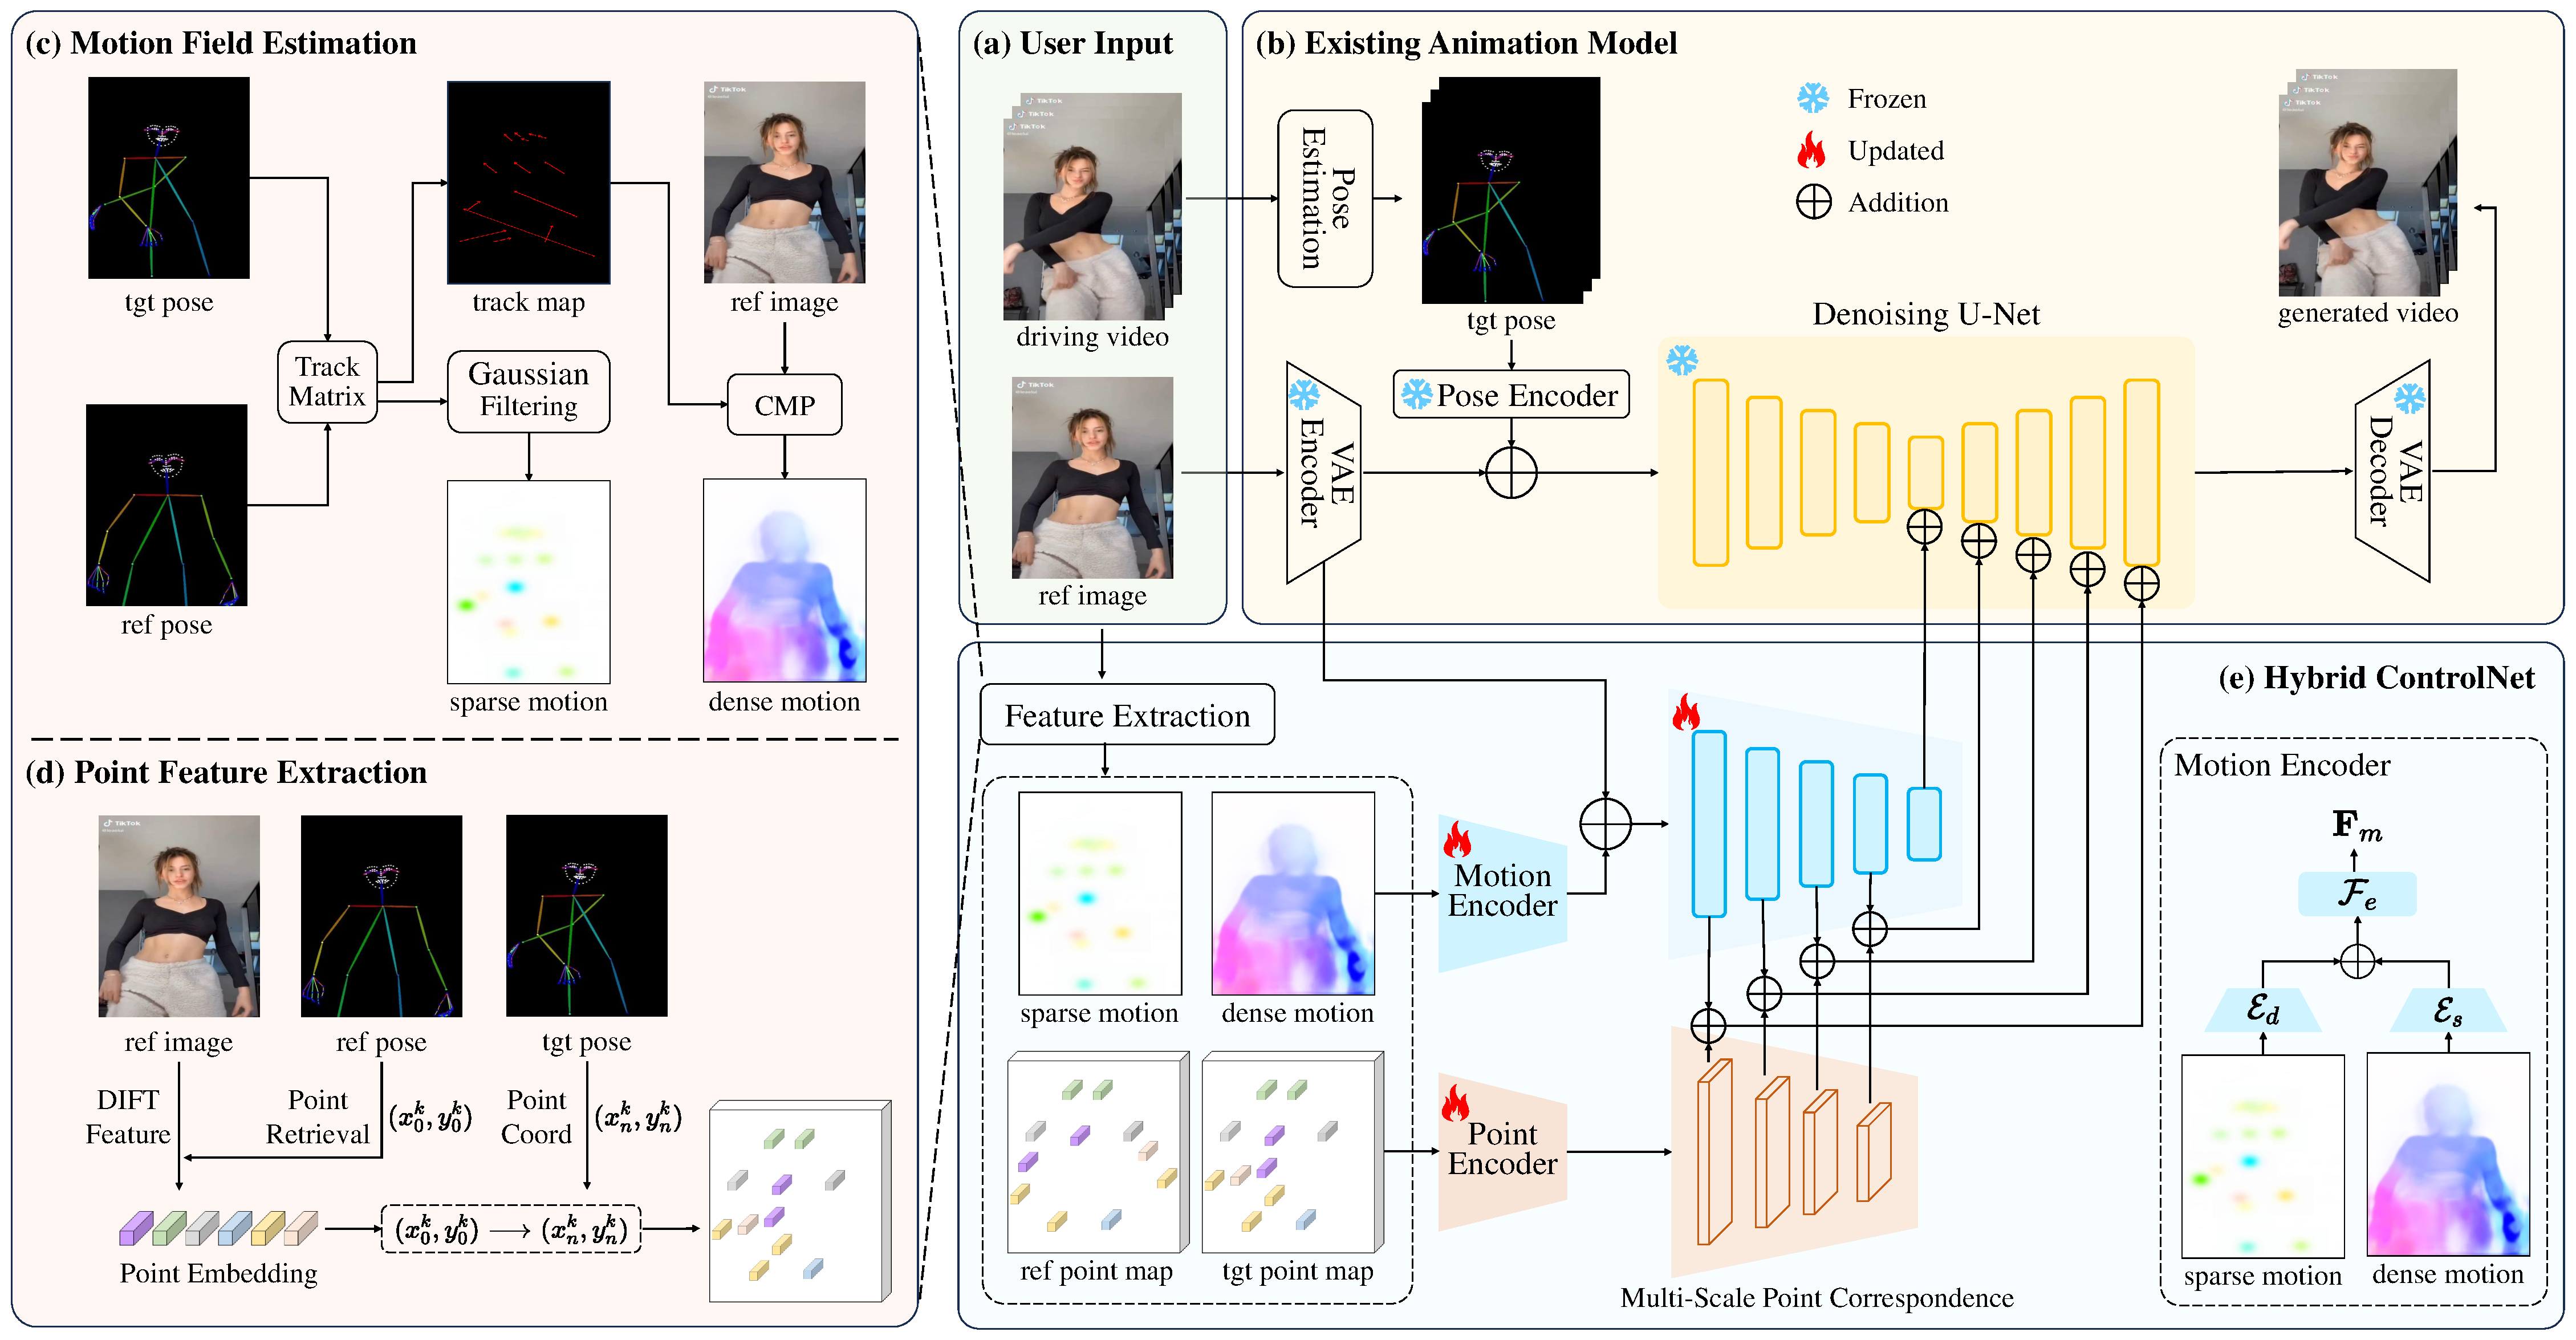
\includegraphics[width=1.0\columnwidth]{./image/pipeline.pdf}
    \vspace{-15pt}
    \caption{The overview of proposed DisPose.}
    \label{fig:pipeline}
\end{figure}
\section{DisPose}
Given a reference image $I_{\mathrm{ref}}\!\in\!\mathbb{R}^{3 \times H \times W}$ and a driving video $V\!\in\!\mathbb{R}^{N\times 3 \times H \times W}$. The core of our method is to disentangle efficient control guidance from only skeleton poses and reference images as shown in Figure~\ref{fig:pipeline}, which can be applied to existing human animation methods without additional dense inputs. We first introduce sparse and dense motion field guides in Sec.~\ref{sec: motion}. Then, we introduce reference-based keypoint correspondence in Sec.~\ref{sec: keypoint}. Finally, we introduce the pipeline of hybrid ControlNet in Sec~\ref{sec: controlnet}.
\subsection{Motion Field Guidance}
\label{sec: motion}

\textbf{Sparse Motion Field.}
We first estimate the skeleton pose by DWpose~\citep{yang2023dwpose} to obtain each frame's human key point coordinates. 
% Subsequently, the motion trajectory of all semantic points in the entire video is obtained and represented as
Subsequently, the key points of the reference image are used as starting points to track the motion displacement of all frames and represented as $P_{traj}\!=\!\{(x^k_n,y^k_n) \!\mid\! k=1\dots K, n=0\dots N\}$, where $P_{traj}$ denotes the trajectory map of the key point $k$ overall $N$ frames and $n = 0$ denotes the reference image. We calculate the track matrix $P_{s}$ as follows:
\begin{equation}
    \mathbf{P}_{s}=\{(x^k_n-x^k_{n-1}, y^k_n-y^k_{n-1}) \mid n=1\dots N\}\},
\end{equation}
% where $P_{t}$ denotes the trajectory map of the key point point $k$ over all $N$ frames, and the reference frame when $n = 0$.
where $K$ denotes the number of keypoints, $N$ denotes the number of frames, $\mathbf{P}_{s}$ denotes the trajectory map of keypoint k over all N frames, and $n = 0$ denotes the reference image.
To avoid training instability caused by overly sparse trajectory matrice, we then apply Gaussian filtering to enhance $\mathbf{P}_{s}$ to obtain the sparse motion field $\mathbf{F}_s\!\in\!\mathbb{R}^{(N-1)\times 2 \times H \times W}$ inspired by~\citep{yin2023dragnuwa, wang2024motionctrl}.

\textbf{Dense Motion Field.}
Considering that sparse control provides limited guidance and dense control is hard to obtain during inference,
% For the dense motion field, 
we transform dense guidance into the motion propagation from the reference frame to the target pose, instead of the dense signal of the target pose. Specifically, in the inference, we reconstruct the trajectory map $\mathbf{P}_{s}$ as the reference-based sparse optical flow $\mathbf{P}_{d}$ from the reference frame to each target pose as:
\begin{equation}
    \mathbf{P}_{d}=\{(x^k_n-x^k_{0}, y^k_n-y^k_{0}) \mid n=1\dots N\}\},
\end{equation}
We then predicted the reference-based dense motion filed $\mathbf{F}_d\!=\! \text{CMP}(P_{traj}, \mathbf{P}_{d}, I_{ref})\!\in\!\mathbb{R}^{(N-1)\times 2 \times H \times W}$ by condition motion propagation (CMP)~\citep{zhan2019self} based on the sparse optical flow $\mathbf{P}_{d}$ and the reference image $I_{ref}$.
CMP~\citep{zhan2019self} is a self-supervised learning-from-motion model that acquires an image and a sparse motion field and estimates the corresponding dense motion field.
Notably, the dense motion field $\mathbf{F}_d$ of each frame starts with the reference image, which avoids geometric constraints during inference.

To ensure motion estimation accuracy during training, we first extract the forward optical flow from the driving video using existing optical flow estimation models~\citep{teed2020raft, xu2023unifying}. We then use a watershed-based approach~\citep{zhan2019self} to sample the sparse optical flow $\mathbf{P}_{d}$ from the forward optical flow. See Appendix.~\ref{sec: appendix1} for details.

\textbf{Motion Encoder.} To leverage motion field as guidance, we introduce a motion encoder specifically designed for the optional flow, which includes sparse motion encoder $\mathcal{E}_s$, dense motion encoder $\mathcal{E}_d$ and feature fusion layer $\mathcal{F}_e$. $\mathcal{E}_d$ and $\mathcal{E}_s$ have the same structure and are multi-scale convolutional encoders with each stage built by \texttt{Conv-SiLU-ZeroConv}~\citep{zhang2023adding} as the basic block. The feature fusion layer $\mathcal{F}_e$ is a 2D convolution for fusing sparse motion features $\mathcal{E}_s(\mathbf{F}_s)$ and dense motion features $\mathcal{E}_d(\mathbf{F}_d)$. Finally, we compute the motion field guidance $\mathbf{F}_m$:
\begin{equation}
    \mathbf{F}_m = \mathcal{F}_e(\mathcal{E}_s(\mathbf{F}_s)+\mathcal{E}_d(\mathbf{F}_d))
\end{equation}

\subsection{Keypoint Correspondence}
\label{sec: keypoint}
\textbf{Point Feature Extraction.} 
To maintain a consistent appearance, it is crucial to correspond the content of the reference image with the motion trajectory. 
Specifically, we first extract the DIFT~\citep{tang2023emergent} features $\mathbf{D}$ of the reference image using the pre-trained image diffusion model. 

Subsequently, the keypoint embedding in the reference is obtained as $\mathbf{D}(x^k_0,y^k_0)$, where $(x^k_0,y^k_0)$ is retrieved from the reference pose.
% key point embeddings $\mathbf{D}(x^k_0,y^k_0)$ are retrieved from $\mathbf{D}$ by skeleton pose $(x^k_0, y^k_0)$.
Next, we initialize the keypoint correspondence map $\mathbf{F}_p$ with zero vectors and assign point embeddings according to the trajectory coordinates as:
\begin{equation}
\label{eq: v prob}
f^{ij}_n=\left\{\begin{array}{ll}
\mathbf{D}(x^k_0,y^k_0), & \mathrm{if} \quad i=x^k_n, j=y^k_n,  \\
0, & \mathrm{otherwise}.
\end{array}\right.
\end{equation}

Finally, we obtain the keypoint correspondence map $\mathbf{F}_p=\{f_n\!\mid\!n=1\dots N\} \!\in\!\mathbb{R}^{N\times D_p \times H \times W}$ for all frames, where $D_p$ is the feature dimension of the point embedding.

\textbf{Point Encoder.} 
To utilize the content correspondence of key points as guidance, we generate multi-scale correspondences of sparse point feature maps and make them compatible with the U-Net encoder of the {Hybrid ControlNet (Sec.4.3)}. 
% as detailed in F. 1.
We introduce the multi-scale point encoder $\mathcal{E}_p$ to maintain the key point content $\mathbf{F}_p$ from the reference image. The point encoder $\mathcal{E}_p$ consists of a series of learnable MLPs.
{
To seamlessly integrate into existing models, we extract intermediate features of the encoder of the hybrid Controlnet.
The multi-scale intermediate features of the Controlnet encoder are denoted as $\mathbf{E}^l_{enc}$, where $l$ denotes each U-Net block $l\!\in\![1, L]$.}
To match the spatial size of $\mathbf{E}^l_{enc}$, we apply downsampling to the feature map between the encoder layers. We compute the multi-scale keypoint correspondence as follows:
\begin{equation}
    \mathbf{F}_c^l = \mathcal{E}_p^l(\phi(\mathbf{F}_p, H^l, W^l)),
\end{equation}
where $(H^l, W^l)$ are denote the spatial dimension of the $l$-th U-Net block and $\phi$ means downsampling operation. Therefore, $\mathbf{F}_c^l$ shares the same size as $\mathbf{E}^l_{enc}$.
Finally, $\mathbf{F}_c$ are added elementwisely to the intermediate feature $\mathbf{E}^l_{enc}$ of the U-Net encoder as guidance: $\mathbf{E}^l_{enc}\!=\!\mathbf{E}^l_{enc}+\mathbf{F}_c^l$.


\subsection{Plug-and-play Hybrid ControlNet}
\label{sec: controlnet}
After obtaining motion field guidance and keypoint correspondence, we aim to integrate these control guidance seamlessly into the U-Net architecture of existing animation models.
Inspired by ControlNet~\citep{zhang2023adding}, We design a hybrid ControlNet $\mathcal{F}$ to provide additional control signals for the existing animation model as shown in Figure~\ref{fig:pipeline}(e).
% Specifically, we consider freeze denoising U-Net and pose encoder. 
Specifically, given an animation diffusion model based on the U-Net architecture, we freeze all its modules while allowing the motion encoder, point encoder and hybrid ControlNet to be updated during training. 
Subsequently, $\mathbf{F}_m$ is added to the noise latent before being input into the hybrid ControlNet. Considering the high sparsity of the point feature $\mathbf{F}_c$, we correspondingly add $\mathbf{F}_c$ to the input of the convolutional layer. Notably, the U-Net encoder intermediate feature $\mathbf{E}_{enc}$ in Sec.~\ref{sec: keypoint} is from hybrid ControlNet rather than denoising U-Net. Finally, 
the control condition is computed as:
\begin{equation}
    \boldsymbol{r}=\mathcal{F}(\boldsymbol{z}_{{t}} \mid \mathbf{F}_m, \mathbf{F}_c, {t})
\end{equation}
where $\boldsymbol{r}$ is a set of condition residuals added to the residuals for the middle and upsampling blocks in the denoising U-Net.

\section{Experiments}
\label{sec:experiments}

We validate our approach empirically, showing that our Monarch matrix parametrization achieves a favorable efficiency--accuracy tradeoff compared to baselines on a wide range of domains (text, images, PDEs, MRI), in three settings (E2E training, S2D training, and D2S fine-tuning):
\begin{itemize}[leftmargin=*,nosep,nolistsep,noitemsep]
\item
In \cref{subsec:benchmark_tasks}, on image classification and language modeling benchmarks, such as ViT / MLP Mixer on ImageNet and GPT-2 on Wikitext-103, Monarch is 2$\times$ faster to train than dense models, while achieving the same accuracy / perplexity. In \cref{subsec:pde_mri}, in scientific and medical domains where special transforms (Fourier) are common, Monarch outperforms Fourier transform based methods on PDE solving, with up to 40\% lower error, and on MRI reconstruction attains up to 15\% higher pSNR and 3.8\% higher SSIM.
\item In \cref{subsec:pde_mri}, we show that on the large OpenWebText dataset, reverse sparsification (training with Monarch weight matrices for most of the time, then transitioning to dense weight matrices) speeds up the pretraining of GPT-2 models by 2$\times$ compared to the dense model, with no loss in upstream or downstream quality.
Moreover, reverse sparsification speeds up BERT pretraining by 23\% even compared to the implementation from Nvidia that set the MLPerf~\citep{mattson2020mlperf} 1.1 record.
\item In \cref{subsec:finetuning}, as a proof of concept, we demonstrate that our Monarch approximation algorithm can improve fine-tuning efficiency for pretrained models. We show that compressing BERT to a Monarch matrix model performs comparably to a finetuned dense model on GLUE, with 2$\times$ fewer parameters and 1.7$\times$ faster finetuning speed.
\end{itemize}

\subsection{End-to-End Training}
\label{subsec:e2e_training}
\subsubsection{Benchmark Tasks: Image Classification, Language Modeling}
\label{subsec:benchmark_tasks}

We show that replacing dense matrices with Monarch matrices in ViT, MLP-Mixer, and
GPT-2 can speed up training by up to 2$\times$ without sacrificing model quality in~\cref{table:pretrain,table:gpt_pretrain}.

\textbf{Setup.} We use the popular vision benchmark, ImageNet~\citep{deng2009imagenet}. We choose recent popular Vision Transformer~\citep{dosovitskiy2020image}, and MLP-Mixer~\citep{tolstikhin2021mlp} as representative base dense models.
For language modeling, we evaluate GPT-2~\citep{radford2019language} on WikiText-103~\citep{merity2016pointer}.

\begin{table}[h]
  \small
  \centering
  \vspace{-2mm}
  \caption{\label{table:pretrain}The performance of Monarch matrices and ViT / MLP-Mixer on ImageNet, including the number of parameters and FLOPs. We measure the Top-1 accuracy and the training time speedup compared to the corresponding dense model. %
  \vspace{2mm}
  }
  \iftoggle{arxiv}{}{
  \resizebox{\linewidth}{!}
  }
  {
  \setlength{\tabcolsep}{3pt}
  \vspace{3em}
  \begin{tabular}{@{}c||ccccccc@{}}
  \specialrule{.15em}{.05em}{.05em}
    Model&\multicolumn{1}{c}{ImageNet acc.}&\multicolumn{1}{c}{Speedup} &\multicolumn{1}{c}{Params} & \multicolumn{1}{c}{FLOPs} \\
    \specialrule{.15em}{.05em}{.05em}
    Mixer-S/16& 74.0& - & 18.5M & 3.8G \\
    Monarch-Mixer-S/16& 73.7& 1.7$\times$ & 7.0M & 1.5G \\
    Mixer-B/16& 77.7& - & 59.9M & 12.6G \\
    Monarch-Mixer-B/16& 77.8& 1.9$\times$ & 20.9M & 5.0G \\
    \specialrule{.15em}{.05em}{.05em}
    ViT-S/16& 79.4 & - & 48.8M & 9.9G \\
    Monarch-ViT-S/16& 79.1 & 1.9$\times$ & 19.6M & 3.9G \\
    ViT-B/16& 78.5 & - & 86.6M  & 17.6G \\
    Monarch-ViT-B/16& 78.9 & 2.0$\times$ & 33.0M & 5.9G \\
    \specialrule{.15em}{.05em}{.05em}
  \end{tabular}
  }
\end{table}

\begin{table}[h]
  \small
  \centering
  \vspace{-3mm}
  \caption{\label{table:gpt_pretrain} Performance of Monarch matrices and GPT-2-Small/Medium on WikiText-103, including the \# of parameters and FLOPs. Monarch achieves similar perplexity (ppl) but 2.0$\times$ faster.}
  \vspace{1mm}
  \iftoggle{arxiv}{}{
    \resizebox{0.95\linewidth}{!}
  }
  {
\setlength{\tabcolsep}{5pt}
\begin{tabular}{c||cccc}
\specialrule{.15em}{.05em}{.05em}
\multirow{1}{*}{{ Model} } & \multicolumn{1}{c}{\multirow{1}{*}{PPL}}
                              & \multicolumn{1}{c}{\multirow{1}{*}{Speedup}}
                              & \multicolumn{1}{c}{\multirow{1}{*}{Params}}
                              & \multicolumn{1}{c}{\multirow{1}{*}{FLOPs}}\\
\specialrule{.15em}{.05em}{.05em}
GPT-2-Small &  20.6 & - & 124M& 106G\\
Monarch-GPT-2-Small& 20.7  & 1.8$\times$ &72M & 51G\\
\specialrule{.15em}{.05em}{.05em}
GPT-2-Medium &  20.9 & - & 355M& 361G\\
Monarch-GPT-2-Medium& 20.3  & 2.0$\times$ &165M & 166G\\
\specialrule{.15em}{.05em}{.05em}
\end{tabular}
}
\vspace{-2mm}
\end{table}


\subsubsection{PDE solving and multi-coil MRI reconstruction}
\label{subsec:pde_mri}

Many scientific or medical imaging tasks rely on specialized transforms such as the
Fourier transform.
We show that replacing the fixed Fourier transform with the more expressive
Monarch matrices yields higher model quality (lower reconstruction error) with
comparable model speed.

\textbf{Solving PDEs with Monarch Neural Operators.}
We follow the experimental setting in FNO~\citep{li2020fourier} and apply a Monarch--based neural operator to the task of solving the Navier--Stokes PDE. Compared to baseline U-Nets~\citep{ronneberger2015u}, TF-Nets~\citep{wang2020towards}, ResNets~\citep{he2016deep} and FNOs~\cite{li2020fourier}, neural operators based on Monarch improve solution accuracy across spatial resolutions by up to $40\%$ (Table \ref{table:pde}).  





\paragraph{Non-periodic boundary conditions.} Traditional spectral methods based on Fourier transform work best with periodic boundary conditions and forcing terms. However, PDEs of practical interest often exhibit non--periodic or even unknown boundary conditions. Monarch operators are not constrained to the Fourier transform and can thus still learn the solution operator with excellent accuracy.

\begin{table}[h!] 
\scriptsize
\vspace{-4mm}
\caption{\label{table:pde}Benchmarks on Navier-Stokes (fixing resolution 64 × 64 for both training and testing).
Decreasing the viscosity coefficient $\nu$ makes the dynamics more chaotic.
}
\vspace{1mm}
\centering
\iftoggle{arxiv}{}{
  \resizebox{0.9\linewidth}{!}
}
{
\renewcommand{\arraystretch}{1}
\begin{tabular}{ c||ccc }
\specialrule{.15em}{.05em}{.05em}
Model & $v = 10^{-3}$  &  $v = 10^{-4}$ & $v = 10^{-5}$\\
\specialrule{.15em}{.05em}{.05em}
U-Net & 0.025  & 0.205  &   0.198\\
TF-Net  & 0.023  & 0.225 &  0.227 \\
ResNet & 0.070 &  0.287 &  0.275 \\
FNO & 0.017  & 0.178 & 0.155\\
Monarch-NO & \textbf{0.010} & \textbf{0.145} & \textbf{0.136} \\
\specialrule{.15em}{.05em}{.05em}
\end{tabular}
}
\textbf{\vspace{-3mm}}
\end{table}

\textbf{Accelerated MRI Reconstruction.} We characterize the utility of Monarch-based FFT operations for accelerated MRI reconstruction, a task which requires methods with both structured Fourier operators and dealiasing properties to recover high quality images. On the clinically-acquired 3D MRI SKM-TEA dataset \citep{desai2021skm}, Monarch-SENSE (mSENSE) enhances image quality by over 1.5dB pSNR and 2.5\% SSIM compared to zero-filled SENSE and up to 4.4dB and 3.8\% SSIM compared to U-Net baselines in data-limited settings. Setup details are available in~\cref{sec:experiment_details_mri}.

\paragraph{Expressive FFT.} By definition, standard IFFT in zero-filled SENSE cannot dealias the signal, resulting in artifacts in the reconstructed image. mSENSE replaces the inverse FFT (IFFT) operation in standard SENSE with learnable Monarch matrices. Thus, mSENSE preserves the structure of the Fourier transform while learning to reweight frequencies to suppress aliasing artifacts. Across multiple accelerations, mSENSE achieved up to +1.5dB and 2.5\% improvement in peak signal-to-noise ratio (pSNR) and structural similarity (SSIM), respectively (Table~\ref{table:mri}).

\paragraph{Data Efficiency.} While CNNs have shown promise for MRI reconstruction tasks, training these networks requires extensive amounts of labeled data to avoid overfitting. However, large data corpora are difficult to acquire in practice. mSENSE can be trained efficiently with limited supervised examples. In few shot settings, mSENSE can outperform U-Net by +4.4dB ($\approx$15\%) and 3.8\% SSIM (Table~\ref{table:mri-data-limited}). 







\begin{table}[h!] 
\scriptsize
\vspace{-3mm}
\caption{\label{table:mri}Mean $\pm$ standard error of the mean of conventional and Monarch-SENSE (mSENSE) on dual-echo (E1,E2) MRI reconstruction at multiple acceleration factors (Acc.).
}
\vspace{1mm}
\centering
\iftoggle{arxiv}{}{
  \resizebox{\linewidth}{!}
}
{
\renewcommand{\arraystretch}{1.2}
\begin{tabular}{c||ccccc}
\specialrule{.15em}{.05em}{.05em}
  & & \multicolumn{2}{c}{pSNR (dB) ($\uparrow$)} & \multicolumn{2}{c}{SSIM ($\uparrow$)} \\
  Acc. & Model &             E1 &             E2 &                E1 &                E2 \\
\specialrule{.15em}{.05em}{.05em}
\multirow{2}{*}{2} & SENSE &  32.8$\pm$0.2 &  35.4$\pm$0.2 &  0.871$\pm$0.003 &  0.865$\pm$0.003 \\
  & mSENSE &  \textbf{34.3$\pm$0.2} &  \textbf{36.6$\pm$0.2} &  \textbf{0.886$\pm$0.002} &  \textbf{0.882$\pm$0.003} \\
\specialrule{.15em}{.05em}{.05em}
\multirow{2}{*}{3} & SENSE &  30.9$\pm$0.2 &  33.5$\pm$0.2 &  0.819$\pm$0.004 &  0.795$\pm$0.004 \\
  & mSENSE &  \textbf{32.3$\pm$0.2} &  \textbf{34.6$\pm$0.2} &  \textbf{0.843$\pm$0.003} &  \textbf{0.820$\pm$0.004} \\
\specialrule{.15em}{.05em}{.05em}
\multirow{2}{*}{4} & SENSE &  30.1$\pm$0.2 &  32.8$\pm$0.2 &  0.789$\pm$0.004 &  0.753$\pm$0.005 \\
  & mSENSE &  \textbf{31.2$\pm$0.2} &  \textbf{33.5$\pm$0.2} &  \textbf{0.812$\pm$0.003} &  \textbf{0.767$\pm$0.005} \\
\specialrule{.15em}{.05em}{.05em}
\end{tabular}
}
\end{table}

\begin{table}[h!] 
\scriptsize
\vspace{-5mm}
\caption{\label{table:mri-data-limited}Impact of number of training examples ($N$) on dual-echo MRI reconstruction at 2x acceleration.
}
\vspace{1mm}
\centering
\iftoggle{arxiv}{}{
  \resizebox{\linewidth}{!}
}
{
\renewcommand{\arraystretch}{1.2}
\begin{tabular}{c||ccccc}
\specialrule{.15em}{.05em}{.05em}
  &  & \multicolumn{2}{c}{pSNR (dB) ($\uparrow$)} & \multicolumn{2}{c}{SSIM ($\uparrow$)} \\
  $N$ & Model &            E1 &            E2 &               E1 &               E2 \\
\specialrule{.15em}{.05em}{.05em}
N/A & SENSE &  32.8$\pm$0.2 &  35.4$\pm$0.2 &  0.871$\pm$0.003 &  0.865$\pm$0.003 \\
\specialrule{.15em}{.05em}{.05em}
\multirow{2}{*}{1} & U-Net &  29.4$\pm$0.2 &  34.4$\pm$0.3 &  0.848$\pm$0.004 &  0.857$\pm$0.004 \\
  & mSENSE &  \textbf{33.8$\pm$0.2} &  \textbf{36.0$\pm$0.2} &  \textbf{0.886$\pm$0.003} &  \textbf{0.867$\pm$0.003} \\
\specialrule{.15em}{.05em}{.05em}
\multirow{2}{*}{2} & U-Net &  29.9$\pm$0.3 &  35.1$\pm$0.3 &  0.858$\pm$0.003 &  0.871$\pm$0.003 \\
  & mSENSE &  \textbf{34.0$\pm$0.2} &  \textbf{36.4$\pm$0.2} &  \textbf{0.883$\pm$0.002} &  \textbf{0.877$\pm$0.003} \\
\specialrule{.15em}{.05em}{.05em}
\multirow{2}{*}{3} & U-Net &  31.0$\pm$0.3 &  35.2$\pm$0.3 &  0.866$\pm$0.003 &  0.867$\pm$0.004 \\
  & mSENSE &  \textbf{33.9$\pm$0.2} & \textbf{ 36.5$\pm$0.2} &  \textbf{0.882$\pm$0.002} & \textbf{0.878$\pm$0.003} \\
\specialrule{.15em}{.05em}{.05em}
\multirow{2}{*}{5} & U-Net &  31.4$\pm$0.3 &  35.6$\pm$0.2 &  0.877$\pm$0.002 &  0.870$\pm$0.003 \\
  & mSENSE &  \textbf{33.9$\pm$0.2} &  \textbf{36.5$\pm$0.2} &  \textbf{0.881$\pm$0.002} &  \textbf{0.877$\pm$0.003} \\
\specialrule{.15em}{.05em}{.05em}
\end{tabular}
}
\end{table}




\subsection{Sparse-to-Dense Training (reverse sparsification)}
\label{subsec:s2d_training}
\paragraph{GPT-2 pretraining.}
On the large OpenWebtext dataset~\citep{Gokaslan2019OpenWeb}, we train a GPT-2 model with Monarch weight
matrices for 90\% of the training iterations, then relax the constraint on the
weight matrices and train them as dense matrices for the remaining 10\% of the
iterations.
We call this technique ``reverse sparsification.''
Previous sparse training techniques often don't speed up training, whereas our
hardware-efficient Monarch matrices do.
Therefore we can use them as an intermediate step to pretrain a large language
model (GPT-2) in 2$\times$ less time. We also evaluate its downstream quality on zero-shot generation from~\citep{eval-harness} and classification tasks from~\citep{zhao2021calibrate}, achieving comparable performance to the dense counterparts (\cref{table:gpt_finetune}). 

\begin{table}[h]
  \small
  \centering
  \vspace{-3mm}
  \caption{\label{table:gpt_finetune}The performance (accuracy) of GPT-2-medium trained with Monarch reverse sparsification and with conventional dense training on text classification benchmarks.}
  \setlength{\tabcolsep}{5pt}
  \vspace{1em}
  \iftoggle{arxiv}{}{
    \resizebox{\linewidth}{!}
  }
  {
  \begin{tabular}{@{}c||ccc@{}}
    \specialrule{.15em}{.05em}{.05em}
    Model&\multicolumn{1}{c}{OpenWebText (ppl)}&\multicolumn{1}{c}{Speedup}& \multicolumn{1}{c}{Classification (avg acc)} \\
    \specialrule{.15em}{.05em}{.05em}
    GPT-2m& 18.0 & - & 38.9 \\
    Monarch-GPT-2m& 18.0 & 2$\times$ & 38.8 \\
    \specialrule{.15em}{.05em}{.05em}
  \end{tabular}
  }
  \vspace{-3mm}
\end{table}


In \cref{fig:reverse_sparsification_bar}, we show the training time of the dense GPT-2 model, along with
the Monarch GPT-2 model.
After training the Monarch model for 90\% of the time, in the
last 10\% of the training steps, by transitioning to dense weight matrices, the model is able to reach the same 
performance of another model that was trained with dense weight matrices from
scratch.
By training with Monarch matrices for 90\% of the time, we reduce the total training time by 2$\times$.

\paragraph{BERT pretraining.}
On the Wikipedia + BookCorpus datasets~\citep{zhu2015aligning}, we train a BERT-large model with Monarch weight matrices for 70\% of the time and transition to dense weight matrices for the remaining 30\% of the time, which yields the same pretraining loss as conventional dense training.
In \cref{table:bert_speed}, we compare the total training time to several baseline implementations: the widely-used implementation from HuggingFace~\citep{wolf-etal-2020-transformers}, the more optimized implementation from Megatron~\citep{shoeybi2019megatron}, and the most optimized implementation we know of from Nvidia that was used to set MLPerf 1.1 training speed record. Our method is 3.5x faster than HuggingFace and 23\% faster than Nvidia's MLPerf 1.1 implementation\footnote{Our result is not an official MLPerf submission. We train BERT for both phase 1 (sequence length 128) and phase 2 (sequence length 512) according to the standard BERT training recipe\cite{devlin2018bert}, while MLPerf only measures training time for phase 2.}.
Experiment details are in~\cref{subsec:bert_details}.

\begin{table}[h]
  \small
  \centering
  \caption{\label{table:bert_speed}The total training time of BERT-large trained with Monarch reverse sparsification and with conventional dense training on 8 A100-40GB GPUs (DGX A100). Training consists of two phases, phase 1 with sequence length 128 and phase 2 with sequence length 512. Monarch training is 3.5x faster than HuggingFace and 23\% faster than Nvidia's MLPerf 1.1 implementation.}
  \vspace{1em}
  \iftoggle{arxiv}{}{
    \resizebox{\linewidth}{!}
  }
  {
    \begin{tabular}{@{}c||c@{}}
      Implementation & Training time (h)  \\ \hline
      HuggingFace &  84.5 \\
      MegaTron & 52.5 \\
      Nvidia MLPerf 1.1 & 30.2 \\
      Nvidia MLPerf 1.1 + DeepSpeed & 29.3 \\
      Monarch (ours) & \textbf{23.8} \\
    \end{tabular}
  }
  \vspace{-3mm}
\end{table}

\subsection{Dense-to-Sparse Fine-tuning}
\label{subsec:finetuning}

\begin{figure}[t]
  \centering
  \vspace{-3mm}
  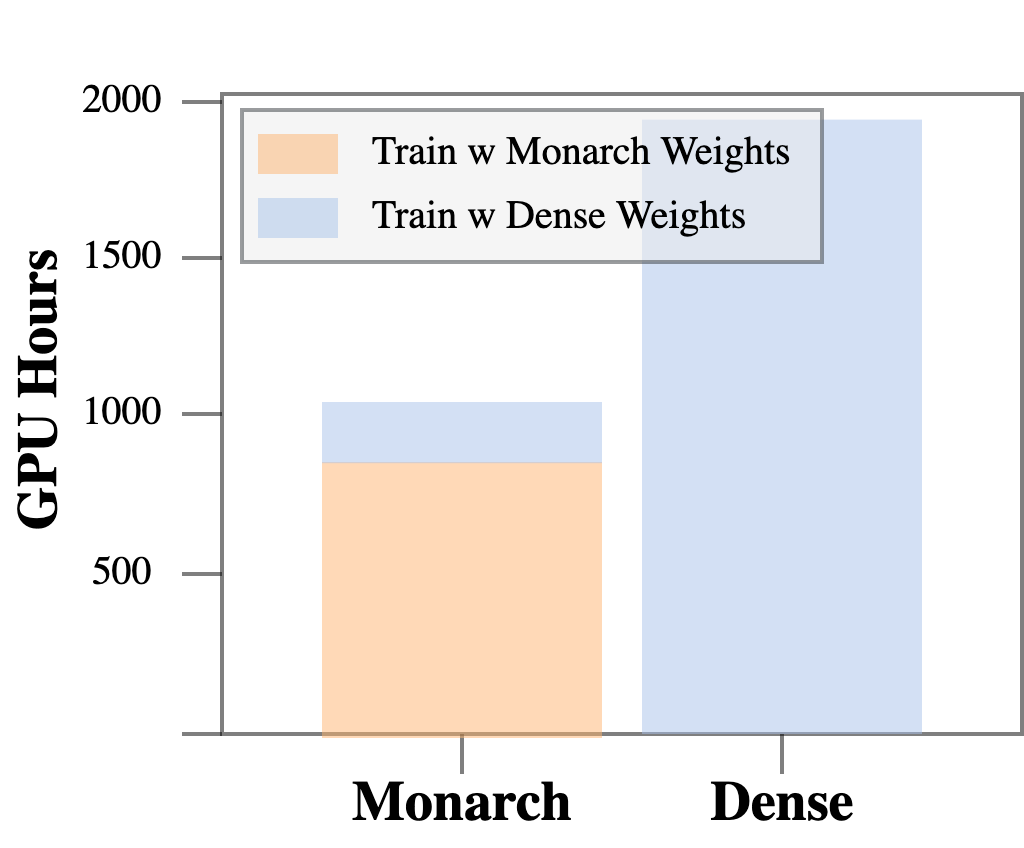
\includegraphics[width=.3\textwidth]{figures/rv_bar_temp.png}
  \vspace{-3mm}
  \caption{\label{fig:reverse_sparsification_bar}Time required (in A100 GPU hours) to reach the same perplexity (18.0)
    for GPT-2-small on OpenWebText.
    With ``reverse sparsification'', Monarch can speed up
    GPT-2 training by 2$\times$.\vspace{-1em}}
\end{figure}

We show that our Monarch approximation algorithm allows us to efficiently use
pretrained models, such as speeding up BERT finetuning on GLUE.

\paragraph{BERT finetuning.}
We take the BERT pretrained weights, approximate them with Monarch matrices,
and finetune the resulting model on the 9 GLUE tasks.
The results in \cref{table:bert_glue} shows that we obtain a Monarch finetuned
model with similar quality to the dense BERT model, but with 1.7$\times$ faster
finetuning speed.
This serves as a proof of concept, and we expect further speedup if additional model compression techniques are applied (e.g., quantization, kernel fusion).




\begin{table}[h]
  \small
  \centering
  \vspace{-5mm}
  \caption{\label{table:bert_glue}The performance of Monarch matrices in
    finetuning BERT on GLUE.}
  \setlength{\tabcolsep}{5pt}
  \vspace{1em}
  \iftoggle{arxiv}{}{
    \resizebox{\linewidth}{!}
  }
  {
  \begin{tabular}{@{}c||ccccccc@{}}
  \specialrule{.15em}{.05em}{.05em}
    Model&\multicolumn{1}{c}{GLUE (avg)}&\multicolumn{1}{c}{Speedup} &\multicolumn{1}{c}{Params} & \multicolumn{1}{c}{FLOPs} \\
    \specialrule{.15em}{.05em}{.05em}
    BERT-base & 78.6& - & 109M & 11.2G \\
    Monarch-BERT-base& 78.3& 1.5$\times$ & 55M & 6.2G  \\
    BERT-large & 80.4 & - & 335M & 39.5G \\
    Monarch-BERT-large & 79.6 & 1.7$\times$ & 144M & 14.6G  \\
    \specialrule{.15em}{.05em}{.05em}
  \end{tabular}
  }
  \vspace{-3mm}
\end{table}





Hyperbolic embeddings embed hierarchical information with high
fidelity and few dimensions. We explored the limits of this approach
by describing scalable, high quality algorithms. We hope the
techniques here encourage more follow-on work on the exciting
techniques of \citet{fb, ucl}. As future work, we hope to explore how
hyperbolic embeddings can be most effectively incorporated into downstream
tasks and applications.


\section*{Acknowledgments}

We thank Laurel Orr, Xun Huang, Trevor Gale, Jian Zhang, Victor Bittorf, Sarah Hooper, Neel Guha, and Michael Zhang for their helpful discussions and feedback on early drafts of the paper.

We gratefully acknowledge the support of NIH under No.\ U54EB020405 (Mobilize), NSF under Nos.\ CCF1763315 (Beyond Sparsity), CCF1563078 (Volume to Velocity), and 1937301 (RTML); ARL under No.\ W911NF-21-2-0251 (Interactive Human-AI Teaming); ONR under No.\ N000141712266 (Unifying Weak Supervision); ONR N00014-20-1-2480: Understanding and Applying Non-Euclidean Geometry in Machine Learning; N000142012275 (NEPTUNE); NXP, Xilinx, LETI-CEA, Intel, IBM, Microsoft, NEC, Toshiba, TSMC, ARM, Hitachi, BASF, Accenture, Ericsson, Qualcomm, Analog Devices, Google Cloud, Salesforce, Total, the HAI-GCP Cloud Credits for Research program,  the Stanford Data Science Initiative (SDSI), and members of the Stanford DAWN project: Facebook, Google, and VMWare. The U.S.\ Government is authorized to reproduce and distribute reprints for Governmental purposes notwithstanding any copyright notation thereon. Any opinions, findings, and conclusions or recommendations expressed in this material are those of the authors and do not necessarily reflect the views, policies, or endorsements, either expressed or implied, of NIH, ONR, or the U.S.\ Government.

\bibliography{ref}
\bibliographystyle{icml2022}


\newpage
\appendix
\onecolumn

\section{Extended Related Work}
\label{app:related}
In this section, we extend the related works referenced in the main paper and discuss them in detail.
\paragraph{Sparse Training.} Our work is loosely related to neural network pruning. By iteratively eliminating neurons and connections, pruning has seen great success in compressing complex models. \citet{han2015deep,han2015learning} put forth two naive but effective algorithms to compress models up to 49x and maintain comparable accuracy. \citet{li2016pruning} employ filter pruning to reduce the cost of running convolution models up to 38 $\%$, \citet{NIPS2017_a51fb975} prunes the network at runtime, hence retaining the flexibility of the full model. \citet{dong2017learning} prunes the network locally in a layer by layer manner.  \citet{sanh2020movement} prunes with deterministic first-order information, which is more adaptive to pretrained model weights. \citet{lagunas2021block} prunes transformers models with block sparsity pattern during fine-tuning, which leads to real hardware speed up while maintaining the accuracy. \citet{zhu2017prune} finds large pruned sparse network consistently outperform the small dense networks with the same compute and memory footprints. Although both our and all the pruning methods are aiming to produce sparse models, we differ in our emphasis on the overall efficiency, whereas pruning mostly focuses on inference efficiency and disregards the cost in finding the smaller model.

There has been more recent work on sparse methods that focuses on speeding up
training and not just inference, such as SNFS~\citep{dettmers2019sparse},
RigL~\citep{dettmers2019sparse}, Top-KAST~\citep{jayakumar2021top}.
These methods often focus on FLOP counts, which may not correlate well with
wall-clock time on modern hardware (e.g., GPUs).
Block-sparsity is another approach that exploits the block-oriented nature of
GPUs~\citep{gray2017gpu, child2019generating, guo2020accelerating}.
Sparse models have also been found useful to improve the training process of
dense models.
For example, sparsity can be used to regularize dense models to improve
accuracy~\citep{han2016dsd}, or to alternate between sparse and dense training
to ease deployment~\citep{peste2021ac}.
Our sparse-to-dense reverse sparsification instead focuses on speeding up dense
training, where the sparse model is used for efficiency and not regularization.


In addition, models proposed in our work can be roughly seen as a class of manually constructed lottery tickets. Lottery tickets \citet{frankle2018lottery} are a set of small sub-networks derived from a larger dense network, which outperforms their parent networks in convergence speed and potentially in generalization. A huge number of studies are carried out to analyze these tickets both empirically and theoretically: \citet{morcos2019one} proposed to use one generalized lottery tickets for all vision benchmarks and got comparable results with the specialized lottery tickets; \citet{frankle2019stabilizing} improves the stability of the lottery tickets by iterative pruning; \citet{frankle2020linear} found that subnetworks reach full accuracy only if they are stable against SGD noise during training; \citet{orseau2020logarithmic} provides a logarithmic upper bound for the number of parameters it takes for the optimal sub-networks to exist; \citet{pensia2020optimal} suggests a way to construct the lottery ticket by solving the subset sum problem and it's a proof by construction for the strong lottery ticket hypothesis. Furthermore, follow-up works \citep{liu2020finding, wang2020picking, tanaka2020pruning} show that we can find tickets without any training labels.


\paragraph{Structured matrices and butterfly matrices.}
Structured matrices are those with asymptotically fast matrix-vector
multiplication algorithm ($o(n^2)$ time complexity) and few parameters ($o(n^2)$
space complexity).
Common examples include sparse \& low-rank matrices, and fast transforms such as
Fourier transform, Chebyshev transform, Legendre transform, and more generally
orthogonal polynomial transforms.
These transforms have been widely used in data preprocessing (e.g., DFT in
speech processing~\citep{jurafsky2014speech}) and kernel
approximation~\citep{le2013fastfood,yu2016orthogonal}.
Many generalizations of these transforms have been used in machine learning to
replace dense weight
matrices~\citep{sindhwani2015structured,thomas2018learning,gu2020hippo}.
\citet{desa2018two} shows that any structured matrix (in the form of arithmetic
circuits) can be written as product of sparse matrices,
and~\citet{dao2020kaleidoscope} shows that products of butterfly matrices can
represent these structured matrices almost optimally in terms of runtime and
memory.
The class of butterfly matrices~\citep{parker1995random} have also been used in
kernel models~\citep{munkhoeva2018quadrature, choromanski2019unifying} and deep
learning models~\citep{vahid2020butterfly,lin2021deformable,
  ailon2021sparse}.

\paragraph{Neural Operators for PDEs.}

Deep learning has found application in the domain of differential equations and scientific computing \cite{rackauckas2020universal}, with methods developed for prediction and control problems \cite{kidger2020neural,massaroli2021differentiable}, as well as acceleration of numerical schemes \cite{poli2020hypersolvers,jolicoeur2021gotta}. Specific to the \textit{partial differential equations} (PDEs) are approaches designed to learn solution operators \cite{raissi2019physics,fan2020solving,li2020fourier}, and hybridized solvers \cite{kochkov2021machine}, evaluated primarily on classical fluid dynamics.

The promise of these approaches is to offer, at the cost of an initial training procedure, accurate yet faster solutions than an appropriate numerical method tuned for a specific problem, which can then be leveraged for real-time forecasting or within larger feedback loops. Nonetheless, optimal design of neural operators remains an open problem, with most relying on fast Fourier transforms (FFT) or standard dense neural architectures. Instead, neural operators based on Monarch are capable of approximating all fast transforms, thus allowing automated optimization towards a suitable transform on a given PDE problem.

\paragraph{MRI.} Accelerated multi-coil MRI is an essential mechanism for reducing long scan times and making certain scan types feasible. In multi-coil MRI, data is acquired in the spatial Fourier domain (a.k.a \textit{k-space}) across multiple coils (sensors). To reduce scan time, this data is sampled below the required rate for recovering the underlying signal (i.e. Nyquist rate), which results in signal aliasing (see Appendix \ref{sec:experiment_details_mri}). In these settings, direct application of the inverse fast Fourier transform (FFT) cannot suppress aliasing artifacts.

Classical MRI reconstruction approaches supplement the FFT by leveraging shared information across multiple coils and strong analytical priors to regularize image recovery objectives. SENSE-based methods jointly dealias images across multiple coils and reweight the final image based on the spatial sensitivity profile of each coil \citep{pruessmann1999sense}. Compressed sensing promotes image sparsity in transformation domains (e.g. Fourier, wavelet) while enforcing data consistency between the Fourier transform of the reconstructed image and the observed measurements \citep{lustig2007sparse}. Low-rank methods enforce low rank structure across slowly-varying dimensions or local patches in the data \citep{ong2016beyond,ravishankar2017low,haldar2013low}. Additionally, GRAPPA-based techniques optimize kernels to directly interpolate missing k-space samples to promote smoothness in the Fourier domain \cite{griswold2002generalized}. Despite their efficacy, these methods have long reconstruction times, require explicit analytical priors, and require careful hyperparameter fine-tuning.

CNNs have shown promise as a fast-at-inference, learnable alternative to classical MRI reconstruction methods \cite{knoll2020deep}. In supervised learning, fully convolutional networks (e.g. U-Net \citep{ronneberger2015u} or unrolled networks \citep{sandino2020compressed,hammernik2018learning}) learn a mapping between paired zero-filled and fully-sampled, ground truth images. However, supervised methods require a large fully-sampled (labeled) data corpus and are sensitive to distribution drifts due to patient, hardware, and sequence heterogeneity \cite{darestani2021measuring}. To reduce dependence on labeled data, unsupervised methods have used generative adversarial networks \citep{cole2020unsupervised, mardani2018deep}, self-supervised learning \cite{yaman2020self}, dictionary learning \cite{lahiri2021blind}, and untrained networks \cite{darestani2021accelerated}. Despite their 
label efficiency, these techniques still underperform supervised methods and are also sensitive to distribution shift. Recently, a family of semi-supervised reconstruction methods demonstrated label efficiency and robustness to physics-driven perturbations, such as changes in signal-to-noise ratio or patient motion \citep{desai2021noise2recon, desai2021vortex}. However, these methods require large amounts of unlabeled data, which can be difficult to curate in few-shot settings. Thus, despite their success in controlled environments, prospective clinical deployment of these models has been stifled \citep{chaudhari2020prospective}.

In our work, we propose a model with a single FFT-initialized factorized Monarch matrix. Such a matrix can provide the benefits of both a simple linearized transformation like FFT and a learnable mechanism to remove aliasing artifacts resulting from the undersampled k-space. The smaller learnable parameter set may reduce overfitting in data-limited settings while preserving the transformation structure of Fourier matrices. Thus, our approach can be interpreted as a hybrid between analytically-constrained classical methods and data-dependent CNNs.


\section{Notation Review}
Throughout this paper, we use lowercase to denote scalars (e.g., $k$), lowercase boldface to denote vectors (e.g., $\vv$), and uppercase boldface to denote matrices (e.g., $\vA$).

$\vI$ denotes the identity matrix. We use $\vA^\top$ to denote the transpose of a matrix and $\vA^*$ to denote the conjugate transpose of a matrix. All results in this paper apply to matrices over the either the reals $\mathbb{R}$ or the complex numbers $\mathbb{C}$; when the field under consideration can be either one of these, we denote it by $\mathbb{F}$.

We use 1-indexing throughout this paper except where explicitly stated.


\newcommand{\baseb}[3]{\parens{{#1},{#2}}_{{#3}}}
\newcommand{\mx}[1]{\mathbf{#1}}
\newcommand{\floors}[1]{\left \lfloor #1 \right \rfloor}
\newcommand{\parens}[1]{\left( {#1}\right)}

\section{General Monarch Matrix Parametrization}
\label{sec:permutation}

In Section \ref{sec:Monarch_square}, we define a parametrization for square Monarch matrices of different ``block sizes'' (i.e., not necessarily $\sqrt{n}$), and prove some basic properties about them. In Section \ref{sec:Monarch_rect}, we further extend this to define rectangular Monarch matrices, and prove some basic properties about them.

Note: In this section, we use 0-indexing rather than 1-indexing, for notational convenience.

\subsection{General square matrices}
\label{sec:Monarch_square}
\subsubsection{Parametrization}
\label{sec:Monarch_square_param}
In this section, we define a more general Monarch parametrization for square matrices, allowing for different ``block sizes.'' Like \cref{def:Monarch}, the parametrization involves the product of a permuted block-diagonal matrix with another block-diagonal matrix; the difference is that we now allow the matrices $\vL$ and $\vR$ to have diagonal blocks of different sizes. Thus, the permutations applied to $\vL$ (to turn it into a block matrix where each block matrix is diagonal) will correspondingly also be different.

First, in \cref{def:square_r}, we define notation for a class of block-diagonal matrices.

\begin{definition}[Class $\BD\ind{b, n}$]
\label{def:square_r}
Let $b \in (1, n)$ be an integer that divides $n$. For $0\le i< \frac {n}{b}$, let $\mx{R}_{i}\in\F^{b \times b }$ be a $b \times b $ ``block" matrix. Then define the matrix $\vR$ with {\em block size} $b$ as follows:
\begin{equation}
 \label{eq:def-R}
  \vR = \diag\left(\vR_0, \dots, \vR_{\frac {n}{b}-1}\right).
\end{equation}
\end{definition}
(Note that the number of possible nonzero values in $\vR$ is $\frac {n}{b}\cdot b^2=nb$.)
We denote the class of all matrices $\vR$ expressible in this form by $\BD\ind{b, n}$. Note that this class is closed under (conjugate) transposition and contains the identity matrix.

Next, in \cref{def:Matrix L}, we define notation for a class of block matrices whose \emph{blocks} are diagonal.

\begin{definition}[Class $\DB\ind{b,n}$]
\label{def:Matrix L}
Let $b \in (1, n)$ be an integer that divides $n$. For $0 \le i, j < b$, let $\mx{D}_{i,j}\in\F^{b\times b}$ be a $b \times b$ diagonal matrix.
Then let $\vL$ be an $n \times n$ matrix with the following form: 
    \begin{equation}
        	\label{eq:def-L}
    \vL=
    	\begin{bmatrix}
    		\mx{D}_{0,0} & \dots & \mx{D}_{0,\frac{n}{b} -1} \\
    		\vdots & \ddots & \vdots \\
    		\mx{D}_{\frac{n}{b} -1,0} & \dots & \mx{D}_{\frac{n}{b} -1,\frac{n}{b} -1}
    	\end{bmatrix}
    \end{equation}
\end{definition}
(Note that the number of possible nonzero values in $\vL$ is $\parens{\frac nb}^2\cdot b=\frac{n^2}b$.)
We denote the class of all matrices $\vL$ expressible in this form by $\DB\ind{b, n}$. Note that this class is closed under (conjugate) transposition and contains the identity matrix. As we show in \cref{sec:sq-Monarch-properties}, $\vL$ can be written as a block-diagonal matrix with $b$ blocks of size $\ff{n}{b} \times \ff{n}{b}$ (i.e., a matrix in $\BD\ind{\frac{n}{b}, \, n}$), multiplied on the left and right with appropriate permutation matrices.
We denote the class of all matrices $\vL$ expressible in this form by $\DB\ind{b, n}$. Note that this class is closed under (conjugate) transposition. As we show in \cref{sec:sq-Monarch-properties}, $\vL$ can be written as a block-diagonal matrix with $b$ blocks of size $\ff{n}{b} \times \ff{n}{b}$ (i.e., a matrix in $\BD\ind{\frac{n}{b}, \, n}$), multiplied on the left and right with appropriate permutation matrices.

Using these two definitions, we define the class of Monarch matrices with a given block size.
\begin{definition}[Class $\M\ind{b,n}$]
\label{def:block_Monarch}
Let $b \in (1, n)$ be an integer that divides $n$. A \emph{Monarch matrix} of size $n \times n$ and ``block size $b$'' is a matrix of the form: 
    \begin{equation}
        	\label{eq:Monarch-general}
    \vM= \vL \vR
    \end{equation}
    where $\vL \in \DB\ind{b,n}$ and $\vR \in \BD\ind{b,n}$.
\end{definition}
We denote the class of all matrices $\vM$ expressible in this form by $\M\ind{b, n}$. Observe that when $b = \sqrt{n}$, this is exactly the matrix class $\M\ind{n}$ in \cref{def:Monarch}. (In other words, $\M\ind{n}$ is shorthand for $\M\ind{\sqrt{n}, n}$.) Note that a matrix in $\M\ind{b,n}$ is represented by $\frac{n^2}{b} + nb$ parameters.

We remark that $\M\ind{b,n} \supset \B\ind{n}$ for all block sizes $b \in (1, n)$ that divide $n$.

Based on \cref{def:block_Monarch}, we define the classes $\M\M^{*(b,n)}$ and $\M^*\M^{(b,n)}$::
\begin{definition}[Class $\M\M^{*(b,n)}$, $\M^*\M^{(b,n)}$]
\label{def:block_MM}
Let $b \in (1, n)$ be an integer that divides $n$ and suppose $\vM_1, \vM_2 \in \M^{(b,n)}$. We define $\M\M^{*(b,n)}$ to be the the class of all matrices $\vM$ expressible in the form $\vM= \vM_1 \vM_2^*$. \newline
We define $\M^*\M^{(b,n)}$ to be the the class of all matrices $\vM$ expressible in the form $\vM= \vM_1^* \vM_2$.
\end{definition}
Observe that when $b = \sqrt{n}$, $\M\M^{*(b,n)}$ is exactly the matrix class $\M\M^{*(n)}$ defined in \cref{sec:theory}. Note that a matrix in $\M\M^{*(b,n)}$ or $\M^*\M\ind{b,n}$. is represented by $2\frac{n^2}{b} + 2nb$ parameters.

Finally, we define the following ``Monarch hierarchy'' based on the kaleidoscope hierarchy of \cite{dao2020kaleidoscope}:
\begin{definition}[Class $(\M\M^{*(b,n)})^w_e$]
\label{def:block_MM}
Let $b \in (1, n)$ be an integer that divides $n$. We define the matrix class $(\M\M^{*(b,n)})^w_e$ as the set of all matrices $\vM$ that can be expressed as
    \begin{equation}
        	\label{eq:mm-hierarchy}
    \vM= \lt \pd{i=1}{w} \vM_i\rt [1:n, 1:n]
    \end{equation}
    where each $\vM_i \in \M\M^{*(b,e\cdot n)}$.
\end{definition}
Note that a matrix in $(\M\M^{*(b,n)})^w_e$ is represented by $2w\frac{e^2n^2}{b} + 2wenb$ parameters.

\subsubsection{Properties}
\label{sec:sq-Monarch-properties}
Here we show some properties of the matrix classes defined above. We first show some basic equivalent ways to define these classes. We then show (\cref{thm:lr_permutation}) that the matrices in $\DB\ind{b, n}$ are permuted block-diagonal matrices; specifically, that they can be converted to matrices in $\BD\ind{\frac{n}{b}, n}$ by applying the appropriate permutation. Finally, we state an expressivity result for the general ``Monarch hierarchy''  which follows from Theorem 1 of \cite{dao2020kaleidoscope}.

First, we define a class of permutations.
Let $1\le b\le n$ be integers such that $b$ divides $n$.
We will need to express each index $0\le i<n$ in ``block form.'' More specifically:

\begin{definition}\label{def:$i$}
Let $i \ge 0$, $b \ge 1$ be integers. Then define
\[i_0=i\mod{b},\]
and
\[i_1=\floors{\frac ib}.\] 
We use the notation $i\equiv\baseb{i_1}{i_0}{b}$ to denote the representation above. In particular, if $i\equiv(i_1,i_0)_{b}$,
then we have
\[
        i = i_1 \cdot b + i_0
\]
\end{definition}

Using this notation, we define the following class of permutations:
\begin{definition}
\label{def:sigma-b}
Let $b \in [1, n]$ be an integer that divides $n$.  Let $i\equiv\baseb{i_1}{i_0}{b}$. Define
    \begin{equation}
            \label{eq:sigma_b-def}
        \sigma_{(b,n)}(i) = i_0\cdot\frac{n}{b} + i_1.
    \end{equation}
That is, $\sigma_{(b,n)}(i)\equiv \baseb{i_0}{i_1}{\frac {n}{b}}$.
Let $\vP_{(b,n)}$ denote the $n \times n$ permutation matrix defined by the permutation $\sigma_{(b,n)}$.
\end{definition}
Intuitively, $\vP_{(b,n)}$ can be interpreted as reshaping a length-$n$ vector into an $b \times \ff{n}{b}$ matrix in row-major order, transposing the result, and then flattening this back into a vector (again in row-major order).


Now, we restate the formulation in \cref{def:square_r} equivalently as:
\begin{proposition}

\label{prop:R-eqv-def}
A matrix $\vR$ satisfies~\Cref{eq:def-R} (i.e., $\vR \in \BD\ind{b,n}$) if and only if the following holds for any
$0\le i,j< n$. Let $i\equiv\baseb{i_1}{i_0}{b}$ and $j\equiv\baseb{j_1}{j_0}{b}$.  Then
\begin{enumerate}
    \item\label{item:zero-loc-R} if $i_1\ne j_1$, then $\vR[i,j]=0$. 
    \item \label{item:nonzero-loc-R} Else (i.e., when $i_1=j_1$), then $\vR[i,j]=\vR_{i_1}[i_0,j_0]$.
\end{enumerate}

\end{proposition}



We restate the formulation in \cref{def:Matrix L} equivalently as:
\begin{proposition}
\label{prop:L-eqv-def}
A matrix $\vL$ satisfies~\Cref{eq:def-L} (i.e., $\vL \in \DB\ind{b,n}$) if and only if the following holds for any
$0\le i,j< n$. Let $i\equiv\baseb{i_1}{i_0}{b}$ and $j\equiv\baseb{j_1}{j_0}{b}$. Then 
\begin{enumerate}
    \item\label{item:zero-loc-L} if $i_0\ne j_0$, then $\vL[i,j]=0$. 
    \item \label{item:nonzero-loc-L} Else, (i.e., when $i_0=j_0$), then $\vL[i,j]=\vD_{i_1,j_1}[i_0,i_0]$.
\end{enumerate}
\end{proposition}

We will argue the following:
\begin{theorem}\label{thm:lr_permutation} Let $1\le b\le n$ such that $b$ divides $n$.
Recall that $\vP_{(b,n)}$ is the permutation matrix defined by the permutation $\sigma_{(b,n)}$. Let $\vL$ be a matrix in $\DB\ind{b, n}$. Then we have
\[\vR'=\vP_{(b,n)}\cdot\vL\cdot\vP_{(b,n)}^\top,\]
where $\vR' \in \BD\ind{\frac{n}{b},\, n}$.
\end{theorem}

\begin{proof}
We first note that multiplying an $n\times n$ matrix on the right (and left resp.) by $\vP_{(b,n)}^\top = \vP_{(\frac nb,n)}$ (and $\vP_{(b,n)}$ resp.) permutes the columns (and rows resp.) of the matrix according to $\sigma_{(b,n)}$.\footnote{This uses the fact that $\parens{\sigma_{(b,n)}}^{-1}=\sigma_{(\frac nb,n)}$ (which means $P_{(\frac{n}{b}, n)} = P_{(b, n)}^\top$ since the inverse of a permutation matrix is its transpose).} This implies that for any $0\le i,j<n$:
\begin{equation}
\label{eq:L-permuted}
\vR'[\sigma_{(b,n)}(i),\sigma_{(b,n)}(j)]=\vL[i,j].
\end{equation}
To complete the proof, we will argue that $\vR'$ satisfies the two conditions in~\Cref{prop:R-eqv-def}.

Towards this end, let $0\le i,j<n$ be arbitrary indices and further, define $i=\baseb{i_1}{i_0}{b}$ and $j=\baseb{j_1}{j_0}{b}$. Then note that $\sigma_{(b,n)}(i)=\baseb{i_0}{i_1}{\frac nb}$ and $\sigma_{(b,n)}(j)=\baseb{j_0}{j_1}{\frac nb}$.

By~\Cref{prop:L-eqv-def}, we have that if $i_0\ne j_0$, then $\vL[i,j]=0$. Note that $i_0\ne j_0$ satisfies the pre-condition for base size $\frac nb$ for indices $(\sigma_{(b,n)}(i),\sigma_{(b,n)}(j))$ in item~\ref{item:zero-loc-R} in~\Cref{prop:R-eqv-def}.  Then   by~\cref{eq:L-permuted}, we have that $\vR'[\sigma_{(b,n)}(i),\sigma_{(b,n)}(j)]=0$, which satisfies item~\ref{item:zero-loc-R} in~\Cref{prop:R-eqv-def}.

Now consider the case that $i_0=j_0$; then by item~\ref{item:nonzero-loc-L} in~\Cref{prop:L-eqv-def}, we have that $\vL[i,j]=\vD_{i_1,j_1}[i_0,i_0]$.  Note that $i_0= j_0$ satisfies the pre-condition for base size $\frac nb$ for indices $(\sigma_{(b,n)}(i),\sigma_{(b,n)}(j))$ in item~\ref{item:nonzero-loc-R} in~\Cref{prop:R-eqv-def} if we define $\vR'_{i_0}\in\F^{\frac nb\times\frac nb}$ as follows:
\[\vR'_{i_0}[i_1,j_1]=\vD_{i_1,j_1}[i_0,i_0].\] 
Note that the above implies that 
\[\vR'=\diag\parens{\vR'_0,\dots,\vR'_{b-1}},\]
where $\vR'_{\cdot}$ is as defined in the above paragraph. This means $\vR' \in \BD\ind{\frac{n}{b}, n}$, since each block $\vR_{i_0}'$ is a matrix of size $\frac{n}{b} \times \frac{n}{b}$.
\end{proof}

We now briefly note some alternate ways to express matrices in $\M\M^{*(b,n)}$.
\begin{proposition}
\label{prop:mm-eqv-def}
For any $\vM \in \M\M^{*(b,n)}$, we can write $\vM = (\vP_{(b,n)}^\top \vL_1 \vP_{(b,n)}) \vR (\vP_{(b,n)}^\top\vL_2\vP_{(b,n)})$, where $\vL_1,\vL_2 \in \BD\ind{\frac{n}{b},n}$ and $\vR \in \BD\ind{b,n}$.
\end{proposition}
\begin{proof}
By definition (see \cref{def:square_r} and \cref{def:Matrix L}), if $\vM \in \M\M^{*(b,n)}$, we can write
$\vM = (\vL_1' \vR_1) (\vL_2' \vR_2)^* = \vL_1' (\vR_1^* \vR_2) \vL_2'^*$,
where $\vL_1',\vL_2' \in \DB\ind{b,n},\vR_1,\vR_2 \in \BD\ind{b,n}$.

Notice that since $\vR_1^*, \vR_2$ are both block-diagonal with the same structure (i.e., both have blocks of size $b \times b$), their product $\vR$ is also in $\BD\ind{b,n}$.
Also, by \cref{thm:lr_permutation} we can write $\vL_1 = \vP_{(b,n)} \vL_1' \vP_{(b,n)}^\top$, $\vL_2 = \vP_{(b,n)} \vL_2' \vP_{(b,n)}^\top$, where $\vL_1,\vL_2$ are both in $\BD\ind{\frac{n}{b},n}$ (i.e., block diagonal with blocks of size $\frac{n}{b} \times \frac{n}{b}$).


Thus, we can write $\vM = (\vP_{(b,n)}^\top \vL_1 \vP_{(b,n)}) \vR (\vP_{(b,n)}^\top\vL_2\vP_{(b,n)})$, where $\vL_1,\vL_2 \in \BD\ind{\frac{n}{b},n}$ and $\vR \in \BD\ind{b,n}$.
\end{proof}

We use the above to show a simple relationship between $\M\M^{*(b,n)}$ and $\M^*\M^{(b,n)}$.
\begin{proposition}
\label{prop:mstarm}
If $\vM \in \M\M^{*(b,n)}$, then $\vP_{(b,n)} \vM \vP_{(b,n)}^\top \in \M^*\M\ind{\frac{n}{b},n}$. Conversely, if $\vM \in \M^*\M^{(b,n)}$, then $\vP_{(b,n)}^\top \vM \vP_{(b,n)} \in \M^*\M\ind{\frac{n}{b},n}$.
\end{proposition}
\begin{proof}
Suppose $\vM \in \M\M^{*(b,n)}$. By \cref{prop:mm-eqv-def} we can write $\vM = (\vP_{(b,n)}^\top \vL_1 \vP_{(b,n)}) \vR (\vP_{(b,n)}^\top\vL_2\vP_{(b,n)})$, where $\vL_1,\vL_2 \in \BD\ind{\frac{n}{b},n}$ and $\vR \in \BD\ind{b,n}$.
Thus $\vP_{(b,n)} \vM \vP_{(b,n)}^\top =
\vL_1 (\vP_{(b,n)} \vR \vP_{(b,n)}^\top) \vL_2$.

Letting $\vL_1' = \vL_1, \vL_2' = \vL_2^*, \vR_1' = \vP_{(b,n)} \vR \vP_{(b,n)}^\top$, and $\vR_2' = \vI$, we have $\vL_1', \vL_2' \in \BD\ind{\frac{n}{b}, n}$, $\vR_1', \vR_2' \in \DB\ind{\frac{n}{b}, n}$, and
$\vL_1 (\vP_{(b,n)} \vR \vP_{(b,n)}^\top) \vL_2 = 
\vL_1' \vR_1' \vR_2'^* \vL_2'^* = (\vL_1' \vR_1')(\vL_2' \vR_2')^* = \vM_1'\vM_2'^*$, where $\vM_1' = \vL_1' \vR_1', \vM_2' = \vL_2' \vR_2'$, so $\vM_1', \vM_2' \in \M^*\M\ind{\frac{n}{b},n}$.

Now instead suppose $\vM \in \M^*\M^{(b,n)}$. So $\vM = \vM_1^* \vM_2 = \vR_1^* \vL_1^* \vL_2 \vR_2$ for some $\vR_1, \vR_2 \in \BD\ind{b,n}$ and $\vL_1, \vL_2 \in \DB\ind{b,n}$. Thus by \cref{thm:lr_permutation} (and the fact that $\BD\ind{b,n}$ is closed under conjugate transposition) we can write $\vR_1^* = \vP_{(\frac{n}{b},n)}^\top \vR_1' \vP_{(\frac{n}{b}, n)} = \vP_{(b,n)} \vR_1' \vP_{(b, n)}^\top$ for some $\vR_1' \in \DB\ind{\frac{n}{b}, n}$, and similarly, can write $\vR_2 = \vP_{(b,n)} \vR_2' \vP_{(b,n)}^\top$ for some $\vR_2' \in \DB\ind{\frac{n}{b}, n}$. 

So $\vP_{(b,n)}^\top \vM \vP_{(b,n)} = \vR_1' (\vP_{(b, n)})^\top \vL_1^*)(\vL_2 \vP_{(b, n)})) \vR_2' =
 \vR_1' (\vP_{(b, n)}^\top \vL_1^* \vP_{(b, n)})(\vP_{(b, n)}^\top \vL_2 \vP_{(b, n)}) \vR_2' = (\vR_1' \vL_1')(\vL_2' \vR_2')$, where $\vL_1' = \vP_{(b, n)}^\top \vL_1^* \vP_{(b, n)}$, $\vL_2' = \vP_{(b, n)}^\top \vL_2 \vP_{(b, n)}$ are in $\BD\ind{\frac{n}{b}, n}$ by \cref{thm:lr_permutation}. Thus letting $\vM_1' = \vR_1'\vL_1'$, $\vM_2' = \vR_2^*\vL_2'^*$, we have $\vM = \vM_1' \vM_2'^*$ with $\vM_1', \vM_2' \in \M^{*(\frac{n}{b},n)}$.
\end{proof}

We now show that the class $\M\ind{b,n}$ strictly contains the class $\B\ind{n}$ of $n \times n$ butterfly matrices (as defined in \citet{dao2020kaleidoscope}). We first show two elementary ``helper'' results.

\begin{proposition}
\label{prop:bd-contain}
If $b,\, c \in (1, n)$ are such that $b$ divides $c$ and $c$ divides $n$, then $\BD\ind{b, n} \subseteq \BD\ind{c, n}$.
\end{proposition}
\begin{proof}
Suppose $\vR \in \BD\ind{b, n}$. Then by \cref{prop:R-eqv-def}, $\vR[i, j] = 0$ whenever $\floor{\frac{i}{b}} \ne \floor{\frac{j}{b}}$. Thus, whenever $\floor{\frac{i}{c}} \ne \floor{\frac{j}{c}}$, $\vR[i, j] = 0$, since $\floor{\frac{i}{c}} \ne \floor{\frac{j}{c}}$ implies $\floor{\frac{i}{b}} \ne \floor{\frac{j}{b}}$ by the assumption that $b$ divides $c$.
Applying \cref{prop:R-eqv-def} again, this means $\vR \in \BD\ind{c,n}$ as well.
\end{proof}

\begin{proposition}
\label{prop:db-contain}
If $b,\, c \in (1, n)$ are such that $b$ divides $c$ and $c$ divides $n$, then $\DB\ind{c, n} \subseteq \DB\ind{b, n}$.
\end{proposition}
\begin{proof}
Suppose $\vL \in \DB\ind{c, n}$. Then by \cref{prop:L-eqv-def}, $\vL[i, j] = 0$ whenever $(i \mod c) \ne (j \mod c)$. Thus, whenever $(i \mod b) \ne (j \mod b)$, $\vL[i, j] = 0$, since $(i \mod b) \ne (j \mod b)$ implies $(i \mod c) \ne (j \mod c)$ by the assumption that $b$ divides $c$.
Applying \cref{prop:L-eqv-def} again, this means $\vL \in \DB\ind{b,n}$ as well.
\end{proof}


\begin{theorem}
\label{thm:b_contained}
Let $n \ge 4$ be a power of 2. The class of matrices $\B\ind{n}$ is a subset of the class $\M\ind{b, n}$, for all $b \in (1, n)$ that divide $n$. When $n \ge 512$ it is a strict subset.
\end{theorem}
\begin{proof}
Recall from \cref{sec:butterfly} that if $\vB \in \B\ind{n}$, it has a \emph{butterfly factorization} 
$\vB = \vB_n \vB_{n/2} \hdots \vB_2$, where each $\vB_i \in \BF\ind{n, i}$.

Consider multiplying together the factors $\vB_b \vB_{b/2} \dots \vB_2$ (where $b \in (1, n)$ divides $n$). Since $\vB_i \in \BF\ind{n,i}$, by definition it is block diagonal with diagonal blocks of size $i \times i$; in other words, $\vB_i \in \BD\ind{i, n}$. Thus, each of the matrices $\vB_b, \vB_{b/2}, \dots, \vB_2$ is in $\BD\ind{b, n}$ (by \cref{prop:bd-contain}), i.e. block-diagonal with block size $b \times b$. This means their product $\vB_b \vB_{b/2} \dots \vB_2$ is also block diagonal with block size $b \times b$, i.e., it is in $\BD\ind{b, n}$.

Now, note that since $\vB_i \in \BF\ind{n,i}$, by definition it is a block matrix with blocks of size $i/2 \times i/2$, where each block is a diagonal matrix (note that some of these blocks are zero, except for the case of $\vB_n$). In other words, $\vB_i \in \DB\ind{i/2, n}$. Thus, for all $i \in \{n, n/2, \dots, 2b\}$, $\vB_i \in \DB\ind{(2b)/2, n} = \DB\ind{b, n}$ (by \cref{prop:db-contain}). So, their product $\vB_n \vB_{n/2} \dots \vB_{2b}$ is in $\DB\ind{b, n}$ as well, as by \cref{thm:lr_permutation} we can write $\vB_n \vB_{n/2} \dots \vB_{2b} = \vP_{(b,n)}^\top (\vP_{(b,n)} \vB_n \vP_{(b,n)}^\top) (\vP_{(b,n)} \vB_{n/2} \vP_{(b,n)}^\top) \dots (\vP_{(b,n)} \vB_{2b} \vP_{(b,n)}^\top) \vP_{(b,n)}$ and each of the $\vP_{(b,n)} \vB_i \vP_{(b,n)}^\top$'s in the preceding expression is in $\BD\ind{\frac{n}{b}, n}$.

Thus, if we let $\vL = \vB_n \vB_{n/2} \dots \vB_{2b}$ and $\vR = \vB_b \vB_{b/2} \dots \vB_2$,  we have $\vB = \vL\vR$ and $\vL \in \DB\ind{b, n}$, $\vR \in \BD\ind{b, n}$, which means that $\vB \in \M\ind{b,n}$ (\cref{def:block_Monarch}).

To show that the inclusion is strict, notice that any $\vM \in \M\ind{b,n}$ is the product of $\vL$ and $\vR$, where $\vR \in \BD\ind{b, n}$ and $\vP_{(b,n)}^\top \vL \vP_{(b,n)} \in \BD\ind{\frac{n}{b}, n}$ (by \cref{thm:lr_permutation}). Notice that the identity matrix is contained in both $\BD\ind{b,n}$ and $\DB\ind{b,n}$. Suppose first that $b \le \sqrt{n}$. Then even if we set $\vR$ to the identity, $\vM$ has at least $\frac{n^2}{b} \ge n^{3/2}$ free parameters (the entries in the blocks of the block-diagonal matrix $\vP_{(b,n)}^\top \vL \vP_{(b,n)}$ can be arbitrary, and there are $b$ such blocks each of size $\frac{n}{b}$). Similarly, in the case $b > \sqrt{n}$, we can set $\vL$ to the identity, and $\vM$ has at least $nb \ge n^{3/2}$ free parameters (the entries of the block-diagonal matrix $\vR$ can be arbitrary, and there are $nb$ total of these). Thus, at least $n^{3/2}$ parameters are required to uniquely describe any matrix in $\M\ind{b,n}$. However, a butterfly matrix in $\B\ind{n}$ has only $2n \log_2 n$ parameters. For $n > 256$, $2n \log_2 n < n^{3/2}$. (Note that this analysis is not tight: a more careful analysis can show the inclusion is strict even for smaller values of $n$.)

\end{proof}

We end this section with a theorem on the expressivity of the ``monarch hierarchy'' (products of monarch matrices), which follows from Theorem 1 of \cite{dao2020kaleidoscope}.
\begin{theorem}[Monarch hierarchy expressivity]
\label{thm:monarch_hierarchy}
Let $\vM$ be an $n \times n$ matrix such that matrix-vector multiplication of $\vM$ and an arbitrary vector $\vv$ (i.e., computation of $\vM \vv$) can
be represented as a linear arithmetic circuit with depth $d$ and $s$ total gates. Let $b \in (1, n)$ be a power of 2 that divides $n$.
Then, $\vM \in (\M\M^{*(b, n)})^{O(d)}_{O(s/n)}$.
\end{theorem}
\begin{proof}
Theorem 1 of \citet{dao2020kaleidoscope} says that if $n$ is a power of 2 and $\vA$ is an $n \times n$ matrix such that multiplying any vector $v$ by $\vA$ can be represented as a linear arithmetic circuit with depth $\le d$ and $\le s$ total gates, then $\vA \in (\B\B^{*(n)})^{O(d)}_{O(s/n)}$ (this is the ``kaleidoscope representation'' of $\vA$).

Recall from \cref{thm:b_contained} that for any $b \in (1, n)$ that is a power of 2 and divides $n$, $\M\ind{b, n} \supset \B\ind{n}$; thus, this implies $\M\M^{*(b,e\cdot n)} \supset \B\B^{*(e\cdot n)}$, and in turn $(\M\M^{*(b,n)})^w_e \supset (\B\B^{*(n)})^w_e$.

As $\vA \in  (\B\B^{*(n)})^{O(d)}_{O(s/n)}$, we thus have $\vA \in  (\M\M^{*(b,n)})^{O(d)}_{O(s/n)}$.
\end{proof}

As per \cite{dao2020kaleidoscope}, the class of kaleidoscope matrices $(\B\B^{*(n)})^{O(d)}_{O(s/n)}$ has $O(ds \log s)$ parameters and runtime, compared to the $O(s)$ parameters and runtime of the circuit. Note that at worst, $s$ is $O(n^2)$.

Define $f(n,s)$ to be the largest power of 2 that is $\le \min\left\{\ff{n}{2}, \sqrt{s}\right\}$. Note that $f(n,s) = O(\sqrt{s})$, and since $s = O(n^2)$, $f(n,s) = \Omega(\sqrt{s})$, so $f(n,s) = \Theta(\sqrt{s})$. %
We thus have $\vA \in (\M\M^{*(f(n,s), n)})^{O(d)}_{O(s/n)}$. The class $(\M\M^{*(f(n,s), n)})^{O(d)}_{O(s/n)}$ has $O(d\frac{s^2}{f(n,s)} + dsf(n,s)) = O(ds^{3/2})$ parameters. Thus, the monarch representation of $\vA$ is suboptimal by at most an $O(d\sqrt{s})$ factor compared to the $O(d{}\,\log s)$ of kaleidoscope.

\subsection{General rectangular matrices}
\label{sec:Monarch_rect}
In this section, we extend the Monarch parametrization to apply to \emph{rectangular} matrices, and prove some basic properties of the relevant matrix classes. (Note that our subsequent theoretical results (\cref{sec:proofs}) do not depend on this section, as they focus on the square parametrization.)

For the rest of the section, we will assume that $n_1, n_2, n_3, b_1, b_2 , b_3 \ge 1$ are integers such that:
\begin{itemize}
\item $b_i$ divides $n_i$ for all $1\le i\le 3$, and 
\item $\frac{n_1}{b_1} = \frac{n_2}{b_2}$.
\end{itemize}

We begin with the definition of the following class of rectangular block-diagonal matrices:
\begin{definition}
\label{def:monarch_rectangular}
For $0\le i< \frac{n}{b_1}$, let $\vR_{i}\in\F^{b_2 \times b_1}$ be a $b_2 \times b_1$ matrix. Then define the matrix $\vR \in \F^{n_2\times n_1}$ as follows:
\begin{equation}
 \label{eq:def-rect-R}
  \vR = \diag\left(\vR_0, \dots, \vR_{\frac {n_1}{b_1}-1}\right).
\end{equation}
\end{definition}
We say that $\vR$ has {\em block size} $b_2 \times b_1$. Recall that we have assumed $\frac {n_1}{b_1}=\frac{n_2}{b_2}$, so~\cref{eq:def-rect-R} is well-defined.
(Note that the number of possible nonzero values in $\vR$ is $\frac {n_1}{b_1}\cdot b_1 \times b_2 =n_1b_2$.)
We denote the class of all matrices $\vR$ expressible in this form by $\BD\ind{b_2 \times b_1, n_2 \times n_1}$.
Note that this class is only defined when $\frac {n_1}{b_1}=\frac{n_2}{n_2}$.



We restate the above definition equivalently as:
\begin{proposition} \label{prop:rect-R-eqv-def} 
$\vR\in\F^{n_2\times n_1}$ is in $\BD\ind{b_2 \times b_1, n_2 \times n_1}$ (with $\frac {n_1}{b_1}=\frac{n_2}{n_2}$) if and only if the following holds for any
$0\le i < n_2$ and $0\le j< n_1$. Let $i\equiv\baseb{i_1}{i_0}{b_2}$ and $j\equiv\baseb{j_1}{j_0}{b_1}$ (recalling this notation from \cref{def:$i$}.  Then
\begin{enumerate}
    \item\label{item:rect-zero-loc-R} if $i_1\ne j_1$, then $\vR[i,j]=0$. 
    \item \label{item:rect-nonzero-loc-R} Else (i.e., when $i_1=j_1$), then $\vR[i,j]=\vR_{i_1}[i_0,j_0]$.
\end{enumerate}

\end{proposition}

Before we define the rectangular $\vL$, we first need to define the notion of a `wrapped diagonal' matrix:
\begin{definition} 
\label{def:wrapped-diag}
A {\em wrapped diagonal} matrix $\mx{S} \in\F^{b_3\times b_2}$ is defined as follows. First assume $b_2\le b_3$. Then for any $0\le i<b_3$ and $0\le j<b_2$, we have the following. If $i\mod{b_2}\ne j$, then $\vS[i,j]=0$. (If $b_2>b_3$, then instead apply the previous definition to $\vS^{\top}$.)

\end{definition}


We now define the following class of block matrices with each block a \emph{wrapped diagonal} matrix.
\begin{definition}\label{def:rect-Matrix L}
Let $\vL\in\F^{n_3\times n_2}$ have the form: 
    \begin{equation}
        	\label{eq:rect-def-L}
    \vL=
    	\begin{bmatrix}
    		\mx{S}_{0,0} & \dots & \mx{S}_{0,\frac{n_2}{b_2} -1} \\
    		\vdots & \ddots & \vdots \\
    		\mx{S}_{\frac{n_3}{b_3} -1,0} & \dots & \mx{S}_{\frac{n_3}{b_3} -1,\frac{n_2}{b_2} -1}
    	\end{bmatrix},
    \end{equation}
where each $\vS_{\cdot,\cdot}$ is a wrapped diagonal matrix in $\F^{b_3 \times b_2}$.
\end{definition}
We say that $\vL$ has {\em block size} $b_3 \times b_2$.
(Note that the number of possible nonzero values in $\vL$ is $\parens{\frac {n_2}{b_2}\cdot \frac{n_3}{b_3}} \max(b_2,b_3)=\frac{n_2 \cdot n_3}{\min(b_2,b_3)}$.)
We denote the class of all matrices $\vL$ expressible in this form by $\DB\ind{b_3 \times b_2, n_3 \times n_2}$.

We restate the above definition equivalently as:


\begin{proposition}
\label{prop:rect-L-eqv-def}
$\vL\in\F^{n_3\times n_2}$ is in $\DB\ind{b_3 \times b_2, n_3 \times n_2}$ if and only if the following holds for any
$0\le i < n_3$ and $0 \le j< n_2$. Let $i\equiv\baseb{i_1}{i_0}{b_3}$ and $j\equiv\baseb{j_1}{j_0}{b_2}$.  Assuming $b_2 \le b_3$, we have:
\begin{enumerate}
    \item\label{item:rect-zero-loc-L} if $i_0\mod{b_2}\ne j_0$, then $\vL[i,j]=0$. 
    \item \label{item:rect-nonzero-loc-L} Else, (i.e., when $i_0\mod{b_2}=j_0$), then $\vL[i,j]=\vS_{i_1,j_1}[i_0,j_0]$.
\end{enumerate}
If $b_2>b_3$, then in the above, the condition ``$i_0\mod{b_2}\ne j_0$'' gets replaced by ``$j_0\mod{b_2}\ne i_0$.''
\end{proposition}

Using the above definitions, we now define the class of rectangular Monarch matrices.
\begin{definition}[Rectangular Monarch Matrix]
\label{def:block_Monarch}
Let $\vM \in \F^{n_3 \times n_1}$ be a matrix of the form: 
    \begin{equation}
        	\label{eq:Monarch-general}
    \vM= \vL \vR
    \end{equation}
    where $\vL \in \DB\ind{b_3 \times b_2, n_3 \times n_2}$ and $\vR \in \BD\ind{b_2 \times b_1, n_2 \times n_1}$.
\end{definition}
(As mentioned before, we assume $b_i$ divides $n_i$ for $i = 1,2,3$ and that $n_1/b_1 = n_2/b_2$.)
We denote the class of all matrices $\vM$ expressible in this form by $\M\ind{(b_1,b_2,b_3), (n_1,n_2,n_3)}$. Observe that when $b_1 = b_2 = b_3 = b$ and $n_1 = n_2 = n_3 = n$, this is exactly the matrix class $\M\ind{b, n}$ in \cref{def:block_Monarch}.

We are now ready to prove our main result in this section, which essentially follows from the observation that if we permute the rows and columns of $\vL$ such that the row/column block size in $\vL$ becomes the number of row/columns blocks in the permuted matrix (and vice-versa) then the permuted matrix has the form of $\vR$.


\begin{theorem} Let $1\le b,n_2,n_3$ be such that $b$ divides $n_2$ and $n_3$.
Suppose $\vL\in\F^{n_3\times n_2} \in \DB\ind{b \times b, n_3 \times n_2}$.
Then if we define
\[\vR'=\vP_{(b,n_3)}\cdot\vL\cdot\vP_{(b,n_2)}^\top,\]
we have that $\vR' \in \BD\ind{\frac{n_3}{b_3} \times \frac{n_2}{b_2}, n_3 \times n_2}$.
\end{theorem}


\begin{proof}
We recall  that multiplying an $m\times n$ matrix on the right (and left resp.) by $\vP_{(b,n)}^\top = \vP_{(\frac nb,n)}$ (and $\vP_{(b,m)}$ resp.) permutes the columns (and rows resp.) of the matrix according to $\sigma_{(b,n)}$ (and $\sigma_{(b,m)}$) respectively.\footnote{This uses the fact that $\parens{\sigma_{(b,n)}}^{-1}=\sigma_{(\frac nb,n)}$.} This implies that for any $0\le i,j<n$:
\begin{equation}
\label{eq:rect-L-permuted}
\vR'[\sigma_{(b,n_3)}(i),\sigma_{(b,n_2)}(j)]=\vL[i,j].
\end{equation}


Recall that in the notation of \cref{def:rect-Matrix L} we have $b_2=b_3=b$, so we are in the $b_2 \le b_3$ case.
To complete the proof, we will argue that $\vR'$ satisfies the two conditions in~\Cref{prop:rect-R-eqv-def}.\footnote{Note that we also need that the ratios of the row/column length to the row/column block sizes are the same; i.e., in our case we need that $\frac{n_3}{n_3 / b_3}=\frac{n_2}{n_2 / b_2}$, which is true because $b_2=b_3=b$.}

Towards this end, let $0\le i,j<n$ be arbitrary indices and further, define $i=\baseb{i_1}{i_0}{b}$ and $j=\baseb{j_1}{j_0}{b}$. Then note that $\sigma_{(b,n_3)}(i)=\baseb{i_0}{i_1}{\frac {n_3}{b}}$ and $\sigma_{(b,n_2)}(j)=\baseb{j_0}{j_1}{\frac {n_2}{b}}$.

By~\Cref{prop:rect-L-eqv-def}, we have that if $i_0\mod{b}\ne j_0$, then $\vL[i,j]=0$. Note  that since $i_0,j_0<b$ by definition, the condition $i_0\mod{b}\ne j_0$ is equivalent to saying $i_0\ne j_0$. Note that $i_0\ne j_0$ satisfies the pre-condition for base size $\frac {n_3}{b}\times \frac{n_2}{b}$ for indices $(\sigma_{(b,n_3)}(i),\sigma_{(b,n_2)}(j))$ in item~\ref{item:rect-zero-loc-R} in~\Cref{prop:rect-R-eqv-def}.  Then   by~\cref{eq:rect-L-permuted}, we have that $\vR'[\sigma_{(b,n_3)}(i),\sigma_{(b,n_2)}(j)]=0$, which satisfies item~\ref{item:rect-zero-loc-R} in~\Cref{prop:rect-R-eqv-def}.

Now consider the case that $i_0=j\mod b$, which by the observation in the above paragraph is the same as $i_0=j_0$. Then by item~\ref{item:rect-nonzero-loc-L} in~\Cref{prop:rect-L-eqv-def}, we have that $\vL[i,j]=\vS_{i_1,j_1}[i_0,j_0]$.  Note that $i_0= j_0$ satisfies the pre-condition for base size $\frac{n_3}{b}\times \frac{n_2}{b}$ for indices $(\sigma_{(b,n_3)}(i),\sigma_{(b,n_2)}(j))$ in item~\ref{item:rect-nonzero-loc-R} in~\Cref{prop:rect-R-eqv-def} if we define $\vR'_{i_0}\in\F^{\frac{n_3}{b}\times\frac{n_2}{b}}$ as follows:
\[\vR'_{i_0}[i_1,j_1]=\vS_{i_1,j_1}[i_0,j_0].\] 

Note that the above implies that 
\[\vR'=\diag\parens{\vR'_0,\dots,\vR'_{b-1}},\]
where $\vR'_{\cdot}$ is as defined in the above paragraph.
This means $\vR' \in \BD\ind{\frac{n_3}{b} \times \frac{n_2}{b}, n_3 \times n_2}$, since $\vR'$ has size $n_3 \times n_2$ and each block $\vR_{i_0}'$ is a matrix of size $\frac{n_3}{b} \times \frac{n_2}{b}$.
\end{proof}

\section{Proofs}

\subsection{Well-behaved activations}
%
The proof of our main results applies to activations that are decent,
i.e.\ well-behaved, in a sense defined in the sequel.  We then show that
$C$-bounded activations as well as the ReLU activation are decent. We
first need to extend the definition of the dual activation and kernel to apply
to vectors in $\reals^d$, rather than just $\mathbb{S}^d$. We denote by
$\cm_+$  the collection of $2\times 2$ positive semi-define matrices and by
$\cm_{++}$ the collection of positive definite matrices.
\begin{definition}
Let $\sigma$ be an activation. Define the following,
\[
\bar\sigma:\cm_{+}^2\to\reals ~~ , ~~
\bar\sigma(\Sigma)=\E_{(X,Y)\sim\gaussian(0,\Sigma)}\sigma(X)\sigma(Y) ~~ , ~~
k_\sigma(\x,\y)=\bar\sigma\begin{pmatrix}
\|\x\|^2 & \inner{\x,\y}
\\
\inner{\x,\y} & \|\y\|^2
\end{pmatrix} \,.
\]
\end{definition}
\noindent
We underscore the following properties of the extension of a
dual activation.
\begin{enumerate}[label=(\alph*)]
\item The following equality holds,
	$$\hat\sigma(\rho)=\bar\sigma\begin{pmatrix}
		1 & \rho \\
		\rho & 1
	\end{pmatrix}$$

\item The restriction of the extended $k_\sigma$ to the sphere agrees
with the restricted definition.

\item The extended dual activation and kernel are defined for every
	activation $\sigma$ such that for all $a\ge 0$, $x\mapsto \sigma(ax)$ is
	square integrable with respect to the Gaussian measure.

\item For $\x,\y\in\reals^d$, if $\w\in\reals^d$ is a multivariate normal
	distribution with zero mean vector and identity covariance matrix,
	then
	$$k_\sigma(\x,\y)=\E_{\w}\sigma(\inner{\w,\x})\sigma(\inner{\w,\y}) \,.$$
\end{enumerate}
Denote
$$\cm^\gamma_+:=\left\{\begin{pmatrix}
\Sigma_{11} & \Sigma_{12}\\
\Sigma_{12} & \Sigma_{22}
\end{pmatrix}\in \cm_+\mid 1-\gamma\le \Sigma_{11},\Sigma_{22}
	\le 1+\gamma\right\} \,. $$
\begin{definition}
A normalized activation $\sigma$ is {\em
$(\alpha,\beta,\gamma)$-decent} for $\alpha,\beta,\gamma\ge 0$ if the
following conditions hold.
\begin{enumerate}[label=(\roman*)]
\item The dual activation $\bar\sigma$ is $\beta$-Lipschitz in
	$\cm_+^\gamma$ with respect to the $\infty$-norm.

\item If $(X_1,Y_1),\ldots,(X_r,Y_r)$ are independent samples from
	$\gaussian\left(0,\Sigma\right)$ for $\Sigma\in \cm_+^\gamma$ then
\[
\Pr\left(\left|\frac{\sum_{i=1}^r\sigma(X_i)\sigma(Y_i)}{r} -
	\bar\sigma(\Sigma)\right|\ge\epsilon\right)
	\le 2\exp\left(-\frac{r\epsilon^2}{2\alpha^2}\right) \,.
\]
\end{enumerate}
\end{definition}

\begin{lemma}[Bounded activations are decent]
	\label{lem:bounded_are_decent}
Let $\sigma:\reals\to\reals$ be a $C$-bounded normalized activation. Then,
$\sigma$ is $(C^2,2C^2,\gamma)$-decent for all $\gamma \ge 0$.
\end{lemma}
\proof
It is enough to show that the following properties hold.
\begin{enumerate}
\item The (extended) dual activation $\bar\sigma$ is $2C^2$-Lipschitz in
	$\cm_{++}$ w.r.t.\ the $\infty$-norm.
\item If $(X_1,Y_1),\ldots,(X_r,Y_r)$ are
 independent samples from $\gaussian\left(0,\Sigma\right)$ then
\[
\Pr\left(\left|\frac{\sum_{i=1}^r\sigma(X_i)\sigma(Y_i)}{r}-\bar\sigma(\Sigma)\right|\ge\epsilon\right) \le 2\exp\left(-\frac{r\epsilon^2}{2C^4}\right)
\]
\end{enumerate}
\noindent
From the boundedness of $\sigma$ it holds that $|\sigma(X)\sigma(Y)| \leq
C^2$. Hence, the second property follows directly from Hoeffding's bound.
We next prove the first part. Let $\z=(x,y)$ and
$\phi(\z) = \sigma(x)\sigma(y)$. Note that for
$\Sigma\in\cm_{++}$ we have
$$\bar\sigma(\Sigma) =
	\frac{1}{2\pi\sqrt{\det(\Sigma)}}
	\int_{\reals^2}\phi(\z)e^{-\frac{\z^\top\Sigma^{-1}\z}{2}}d\z \,.$$
Thus we get that,
\begin{eqnarray*}
\frac{\partial \bar\sigma}{\partial \Sigma} &=&
	\frac{1}{2\pi}\int_{\reals^2}
		\phi(\z)\left[
			\frac{\frac{1}{2}\sqrt{\det(\Sigma)}\Sigma^{-1} -
				\frac{1}{2}\sqrt{\det(\Sigma)}(\Sigma^{-1}\z\z^\top\Sigma^{-1})}
				{\det(\Sigma)}
						\right]
		e^{-\frac{\z^\top\Sigma^{-1}\z}{2}}d\z
\\
&=& \frac{1}{2\pi\sqrt{\det(\Sigma)}}\int_{\reals^2}\phi(\z)\frac{1}{2}\left[
\Sigma^{-1}-\Sigma^{-1}\z\z^\top\Sigma^{-1}
\right]e^{-\frac{\z^\top\Sigma^{-1}\z}{2}}d\z
\end{eqnarray*}
Let $g(\z)=e^{-\frac{\z^\top\Sigma^{-1}\z}{2}}$. Then, the first and second
order partial derivatives of $g$ are
\begin{eqnarray*}
\frac{\partial g}{\partial \z} & = &
	-\Sigma^{-1}\z e^{-\frac{\z^\top\Sigma^{-1}\z}{2}} \\
\frac{\partial^2 g}{\partial^2 \z} & = &
	\left[-\Sigma^{-1} +
		\Sigma^{-1}\z\z^\top\Sigma^{-1}\right]e^{-\frac{\z^\top\Sigma^{-1}\z}{2}} \,.
\end{eqnarray*}
We therefore obtain that,
\[
\frac{\partial \bar\sigma}{\partial \Sigma} =
	-\frac{1}{4\pi\sqrt{\det(\Sigma)}} \int_{\reals^2}
		\phi\frac{\partial^2 g}{\partial^2 \z} d\z \,.
\]
By the product rule we have
\[
\frac{\partial \bar\sigma}{\partial \Sigma} =
-\frac{1}{2\pi\sqrt{\det(\Sigma)}}\frac{1}{2}\int_{\reals^2}\frac{\partial^2
\phi}{\partial^2 \z} gd\z = -\frac{1}{2}\E_{(X,Y)\sim\gaussian(0,\Sigma)}\left[\frac{\partial^2 \phi}{\partial^2 \z}(X,Y)\right]
\]
We conclude that $\bar\sigma$ is differentiable in $\cm_{++}$ with
partial derivatives that are point-wise bounded by $\frac{C^2}{2}$. Thus,
$\bar\sigma$ is $2C^2$-Lipschitz in $\cm_+$ w.r.t.\ the $\infty$-norm. \qed

\medskip
We next show that the ReLU activation is decent.
\begin{lemma}[ReLU is decent]\label{lem:relu_is_decent}
%
There exists a constant $\alpha_\mathrm{ReLU}\ge 1$ such that for
$0\le \gamma\le 1$, the normalized ReLU activation
$\sigma(x)=\sqrt{2}\max(0,x)$ is
$(\alpha_\mathrm{ReLU},1+o(\gamma),\gamma)$-decent.
\end{lemma}
\proof
The measure concentration property follows from standard concentration
bounds for sub-exponential random variables (e.g.\ ~\cite{shalev2014understanding}).  It
remains to show that $\bar\sigma$ is $(1+o(\gamma))$-Lipschitz in
$\cm^\gamma_+$. We first calculate an exact expression for $\bar\sigma$.
The expression was already calculated in~\cite{cho2009kernel}, yet we give
here a derivation for completeness.
%
\begin{claim}\label{claim:relu_dual_ext}
The following equality holds for all $\Sigma\in\cm_{+}^2$,
$$\bar\sigma(\Sigma) = \sqrt{\Sigma_{11}\Sigma_{22}} \,
	\hat\sigma\!\left(\frac{\Sigma_{12}}{\sqrt{\Sigma_{11}\Sigma_{22}}}\right)
\,. $$
\end{claim}
\proof Let us denote
$$\tilde{\Sigma} = \begin{pmatrix}
1 & \frac{\Sigma_{12}}{\sqrt{\Sigma_{11}\Sigma_{12}}} \\
\frac{\Sigma_{12}}{\sqrt{\Sigma_{11}\Sigma_{12}}} & 1
\end{pmatrix} \,. $$
By the positive homogeneity of the ReLU activation we have
\begin{eqnarray*}
\bar\sigma\left(\Sigma\right) &=&
	\E_{(X,Y)\sim\gaussian(0,\Sigma)}\sigma(X)\sigma(Y) \\
&=& \sqrt{\Sigma_{11}\Sigma_{22}}
		\E_{(X,Y)\sim\gaussian(0,\Sigma)}
			\sigma\!\left(\frac{X}{\sqrt{\Sigma_{11}}}\right)
			\sigma\!\left(\frac{Y}{\sqrt{\Sigma_{22}}}\right) \\
&=& \sqrt{\Sigma_{11}\Sigma_{22}}
			\E_{(\tilde{X},\tilde{Y})\sim\gaussian\left(0,\tilde{\Sigma}\right)}
			\sigma\!\left(\tilde{X}\right)\sigma\!\left(\tilde{Y}\right) \\
&=& \sqrt{\Sigma_{11}\Sigma_{22}}\,
	\hat{\sigma}\!\left(\frac{\Sigma_{12}}{\sqrt{\Sigma_{11}\Sigma_{22}}}\right)
	\, .
\end{eqnarray*}
which concludes the proof. \qed

\medskip

For brevity, we henceforth drop the argument from $\bar{\sigma}(\Sigma)$ and
use the abbreviation $\bar{\sigma}$. In order to show that $\bar\sigma$ is
$(1+o(\gamma))$-Lipschitz w.r.t.\ the $\infty$-norm it is enough to show that
for every $\Sigma\in\cm_+^\gamma$ we have,
\begin{equation}\label{eq:grad_l1_bound}
\|\nabla \bar \sigma\|_1 =
	\left|\frac{\partial \bar\sigma}{\partial \Sigma_{12}}\right| +
	\left|\frac{\partial \bar\sigma}{\partial \Sigma_{11}}\right| +
	\left|\frac{\partial \bar\sigma}{\partial \Sigma_{22}}\right|\le
		1+o(\gamma) \,.
\end{equation}
First, Note that ${\partial \bar\sigma}/{\partial \Sigma_{11}}$ and
${\partial \bar\sigma}/{\partial \Sigma_{22}}$ have the same sign,
hence,
$$\|\nabla \bar \sigma\|_1 =
	\left|\frac{\partial \bar\sigma} {\partial \Sigma_{12}}\right| +
	\left|\frac{\partial \bar\sigma}{\partial \Sigma_{11}} +
				\frac{\partial \bar\sigma}{\partial \Sigma_{22}}\right| \,.$$
Next we get that,
\begin{eqnarray*}
\frac{\partial \bar\sigma}{\partial \Sigma_{11}} & = &
	\frac{1}{2}\sqrt{\frac{\Sigma_{22}}{\Sigma_{11}}}\,
	\hat\sigma\!\left(\frac{\Sigma_{12}}{\sqrt{\Sigma_{11}\Sigma_{22}}}\right) -
	\frac{1}{2}\sqrt{\frac{\Sigma_{22}}{\Sigma_{11}}}
		\frac{\Sigma_{12}}{\sqrt{\Sigma_{11}\Sigma_{22}}}\,
		\hat\sigma'\!\left(\frac{\Sigma_{12}}{\sqrt{\Sigma_{11}\Sigma_{22}}}\right)
\\
\frac{\partial \bar\sigma}{\partial \Sigma_{22}} & = &
	\frac{1}{2}\sqrt{\frac{\Sigma_{11}}{\Sigma_{22}}}\,
	\hat\sigma\!\left(\frac{\Sigma_{12}}{\sqrt{\Sigma_{11}\Sigma_{22}}}\right) -
	\frac{1}{2}\sqrt{\frac{\Sigma_{11}}{\Sigma_{22}}}
	\frac{\Sigma_{12}}{\sqrt{\Sigma_{11}\Sigma_{22}}}\,
	\hat\sigma'\!\left(\frac{\Sigma_{12}}{\sqrt{\Sigma_{11}\Sigma_{22}}}\right)
\\
\frac{\partial \bar\sigma}{\partial \Sigma_{12}} & = &
	\hat\sigma'\!\left(\frac{\Sigma_{12}}{\sqrt{\Sigma_{11}\Sigma_{22}}}\right)
	\, .
\end{eqnarray*}
We therefore get that the $1$-norm of $\nabla\bar\sigma$ is,
\[
\|\nabla \bar \sigma\|_1 =
\frac{1}{2}\frac{\Sigma_{11}+\Sigma_{22}}{\sqrt{\Sigma_{11}\Sigma_{22}}}
\left|
	\hat\sigma\!\left(\frac{\Sigma_{12}}{\sqrt{\Sigma_{11}\Sigma_{22}}}\right) -
	\frac{\Sigma_{12}}{\sqrt{\Sigma_{11}\Sigma_{22}}}\,
	\hat\sigma'\!\left(\frac{\Sigma_{12}}{\sqrt{\Sigma_{11}\Sigma_{22}}}\right)
\right| +
	\hat\sigma'\!\left(\frac{\Sigma_{12}}{\sqrt{\Sigma_{11}\Sigma_{22}}}\right)
	\,.
\]
The gradient of
$\frac{1}{2}\frac{\Sigma_{11}+\Sigma_{22}}{\sqrt{\Sigma_{11}\Sigma_{22}}}$
at $(\Sigma_{11},\Sigma_{22})=(1,1)$ is $(0,0)$. Therefore, from the mean
value theorem we get,
$\frac{1}{2}\frac{\Sigma_{11}+\Sigma_{22}}{\sqrt{\Sigma_{11}\Sigma_{22}}} =
	1+o(\gamma)$.
Furthermore, $\hat\sigma$, $\hat\sigma'$ and
$\frac{\Sigma_{12}}{\sqrt{\Sigma_{11}\Sigma_{22}}}$ are bounded by $1$ in
absolute value. Hence, we can write,
\[
\|\nabla \bar \sigma\|_1 =
\left|
\hat\sigma\!\left(\frac{\Sigma_{12}}{\sqrt{\Sigma_{11}\Sigma_{22}}}\right) -
\frac{\Sigma_{12}}{\sqrt{\Sigma_{11}\Sigma_{22}}}
\hat\sigma'\!\left(\frac{\Sigma_{12}}{\sqrt{\Sigma_{11}\Sigma_{22}}}\right)
\right| +
\hat\sigma'\!\left(\frac{\Sigma_{12}}{\sqrt{\Sigma_{11}\Sigma_{22}}}\right)
+ o(\gamma) \,.
\]
Finally, if we let $t=\frac{\Sigma_{12}}{\sqrt{\Sigma_{11}\Sigma_{22}}}$,
we can further simply the expression for $\nabla\bar\sigma$,
\begin{eqnarray*}
\|\nabla \bar \sigma(\Sigma)\|_1 &=& |\hat\sigma(t)-t\hat\sigma'(t)| + |\hat\sigma'(t)|  + o(\gamma)
\\
&=& \frac{\sqrt{1-t^2}}{\pi} + 1 - \frac{\cos^{-1}(t)}{\pi}  + o(\gamma) \,.
\end{eqnarray*}
Finally, the proof is obtained from the fact that the function $f(t)=\frac{\sqrt{1-t^2}}{\pi} + 1 - \frac{\cos^{-1}(t)}{\pi}$ satisfies $0\le f(t)\le 1$ for every $t\in [-1,1]$.
Indeed, it is simple to verify that $f(-1)=0$ and $f(1)=1$. Hence, it suffices to
show that $f'$ is non-negative in $[-1,1]$ which is indeed the case since,
\[
f'(t) = \frac{1}{\pi}\frac{1-t}{\sqrt{1-t^2}} =
	\frac{1}{\pi}\sqrt{\frac{1-t}{1+t}} \ge 0 \,. \qedhere
\]

\subsection{Proofs of Thms.~\ref{thm:main_ker}~and~\ref{thm:main_ker_ReLU}}
We start by an additional theorem which serves as a simple stepping stone
for proving the aforementioned main theorems.
\begin{theorem}\label{thm:ker_appr}
%
Let $\cs$ be a skeleton with $(\alpha,\beta,\gamma)$-decent
activations, $0<\epsilon \le \gamma$, and
$B_d = \sum_{i=0}^{d-1}\beta^i$. Let $\w$ be a random initialization of the
network $\cn=\cn(\cs,r)$ with
$$r \ge \frac{2\alpha^2B_{\depth(\cs)}^2
	\log\left(\frac{8|\cs|}{\delta}\right)} {\epsilon^2} \,. $$
Then, for every $\x,\y$ with probability of at least $1-\delta$, it holds that
\[
|\kappa_\w(\x,\y)-\kappa_\cs(\x,\y)|\le \epsilon \,.
\]
\end{theorem}
\noindent
Before proving the theorem we show that together with
Lemmas~\ref{lem:bounded_are_decent}~and~\ref{lem:relu_is_decent},
Theorems~\ref{thm:main_ker}~and~\ref{thm:main_ker_ReLU} follow from
Theorem~\ref{thm:ker_appr}. We restate them as corollaries, prove them,
and then proceed to the proof of Theorem \ref{thm:ker_appr}.
\begin{corollary}
Let $\cs$ be a skeleton with $C$-bounded activations. Let $\w$ be a random
initialization of $\cn=\cn(\cs,r)$ with
$$r \ge \frac{(4C^4)^{\depth(\cs)+1}
\log\left(\frac{8|\cs|}{\delta}\right)}{\epsilon^2} \,.$$
Then, for every $\x,\y$, w.p.\ $\ge 1-\delta$,
\[
|\kappa_\w(\x,\y)-\kappa_\cs(\x,\y)|\le \epsilon\,.
\]
\end{corollary}
\proof
From Lemma~\ref{lem:bounded_are_decent}, for all $\gamma>0$, each
activation is $(C^2,2C^2,\gamma)$-decent. By Theorem
\ref{thm:ker_appr}, it suffices to show that
$$2\left(C^2\right)^2\left(\sum_{i=0}^{\depth(\cs)-1}(2C^2)^{i}\right)^2
	\le (4C^4)^{\depth(\cs)+1} \,. $$
The sum of can be bounded above by,
\[
\sum_{i=0}^{\depth(\cs)-1}\!\!\!(2C^2)^{i} =
	\frac{(2C^2)^{\depth(\cs)}-1}{2C^2-1} \le
	\frac{(2C^2)^{\depth(\cs)}}{C^2} \,.
\]
Therefore, we get that,
\[
2\left(C^2\right)^2\left(\sum_{i=0}^{\depth(\cs)-1}\!\!\!(2C^2)^{i}\right)^2
	\le \frac{2C^4(4C^4)^{\depth(\cs)}}{C^4} \le (4C^4)^{\depth(\cs)+1} \,,
\]
which concludes the proof. \qed

\begin{corollary}
Let $\cs$ be a skeleton with ReLU activations, and $\w$ a random
initialization of $\cn(\cs,r)$ with $r \ge c_1 \frac{\depth^2(\cs)
\log\left(\frac{8|\cs|}{\delta}\right)}{\epsilon^2}$. For all $\x,\y$ and
$\epsilon\le \min(c_2,\frac{1}{\depth(\cs)})$, w.p.\ $\ge 1-\delta$,
	\[
	|\kappa_\w(\x,\y)-\kappa_\cs(\x,\y)|\le \epsilon
	\]
	Here, $c_1,c_2>0$ are universal constants.
\end{corollary}
\proof
From Lemma \ref{lem:relu_is_decent}, each activation is
$(\alpha_{\mathrm{ReLU}},1+o(\epsilon),\epsilon)$-decent. By Theorem
\ref{thm:ker_appr}, it is enough to show that
$$\sum_{i=0}^{\depth(\cs)-1}\!\!\!(1+o(\epsilon))^{i}=O(\depth(\cs)) \,.$$
This claim follows from the fact that
$(1+o(\epsilon))^{i}\le e^{o(\epsilon)\depth(\cs)}$ as long as
$i\le \depth(\cs)$. Since we assume that
$\epsilon\le{1}/{\depth(\cs)}$, the expression is bounded by $e$
for sufficiently small $\epsilon$.
\proofbox

\medskip

\noindent We next prove Theorem \ref{thm:ker_appr}.
\proof (Theorem \ref{thm:ker_appr})
For a node $u\in\cs$ we denote by $\Psi_{u,\w}:\cx\to\reals^r$ the normalized
representation of $\cs$'s sub-skeleton rooted at $u$.
Analogously, $\kappa_{u,\w}$ denotes the empirical kernel of that network.
When $u$ is the output node of $\cs$ we still use $\Psi_{\w}$ and $\kappa_\w$
for $\Psi_{u,\w}$ and $\kappa_{u,\w}$. Given two fixed $\x,\y\in\cx$ and a node
$u\in\cs$, we denote
\[
\mathcal{K}_\w^u=
\begin{pmatrix}
\kappa_{u,\w}(\x,\x) &
\kappa_{u,\w}(\x,\y)
\\
\kappa_{u,\w}(\x,\y) &
\kappa_{u,\w}(\y,\y)
\end{pmatrix},\;\; \mathcal{K}^u = \begin{pmatrix}
\kappa_u(\x,\x) & \kappa_u(\x,\y)
\\
\kappa_u(\x,\y) & \kappa_u(\y,\y)
\end{pmatrix}
\]
\[
\mathcal{K}_\w^{\leftarrow u}=\frac{\sum_{v\in\IN(u)}\mathcal{K}^{v}_\w}{|\IN(u)|}
,\quad \mathcal{K}^{\leftarrow u}=\frac{\sum_{v\in\IN(u)}\mathcal{K}^{v}}{|\IN(u)|} \,.
\]
For a matrix $\mathcal{K}\in\cm_+$ and a function $f:\cm_+\to\reals$, we denote
\[
f^p(\mathcal{K})=\begin{pmatrix}
f\!\begin{pmatrix}
\mathcal{K}_{11} & \mathcal{K}_{11}
\\
\mathcal{K}_{11} & \mathcal{K}_{11}
\end{pmatrix} & f(\mathcal{K})
\\
f(\mathcal{K}) & f\!\begin{pmatrix}
\mathcal{K}_{22} & \mathcal{K}_{22}
\\
\mathcal{K}_{22} & \mathcal{K}_{22}
\end{pmatrix}
\end{pmatrix}
\]
Note that $\mathcal{K}^u=\bar\sigma_u^p(\mathcal{K}^{\leftarrow u})$.
We say that a node $u\in \cs$, is {\em well-initialized} if
\begin{equation}\label{eq:1}
\|\mathcal{K}_\w^u- \mathcal{K}^u\|_\infty
	\le \epsilon\frac{B_{\depth(u)}}{B_{\depth(\cs)}} \,.
\end{equation}
Here, we use the convention that $B_{0}=0$. It is enough to show that with
probability of at least $\ge 1-\delta$ all nodes are well-initialized. We first note that input nodes are well-initialized by construction since
$\mathcal{K}^u_\w=\mathcal{K}^u$. Next, we show that given that all incoming
nodes for a certain node are well-initialized, then w.h.p.\ the node is
well-initialized as well.
\begin{claim}\label{claim1}
Assume that all the nodes in $\IN(u)$ are well-initialized. Then, the node
$u$ is well-initialized with probability of at least $1-\frac{\delta}{|\cs|}$.
\end{claim}
\proof
It is easy to verify that $\mathcal{K}_\w^u$ is the empirical
covariance matrix of $r$ independent variables distributed according to
$\left(\sigma(X),\sigma(Y)\right)$ where
$(X,Y)\sim\gaussian\left(0,\mathcal{K}_\w^{\leftarrow u}\right)$.
Given the assumption that all nodes incoming to $u$ are well-initialized,
we have,
\begin{eqnarray}\label{eq:2}
\left\|\mathcal{K}_\w^{\leftarrow u}-\mathcal{K}^{\leftarrow u}\right\|_\infty
&=&
\left\|
	\frac{\sum_{v\in\IN(v)}\mathcal{K}_\w^{v}}{|\IN(v)|} -
	\frac{\sum_{v\in\IN(v)}\mathcal{K}^{v}}{|\IN(v)|}\right\|_\infty\nonumber
\\
&\le& \frac{1}{|\IN(v)|}\sum_{v\in\IN(v)}
	\left\|\mathcal{K}_\w^{v}-\mathcal{K}^{v}\right\|_\infty
\\
&\le&  \epsilon\frac{B_{\depth(u)-1}}{B_{\depth(\cs)}}\nonumber \,.
\end{eqnarray}
Further, since $\epsilon\le \gamma$ then
$\mathcal{K}^{\leftarrow u}_\w\in \cm_+^\gamma$. Using the fact
that $\sigma_u$ is
$(\alpha,\beta,\gamma)$-decent and that
$r\ge \frac{2\alpha^2 B^2_{\depth(\cs)}
	\log\left(\frac{8|\cs|}{\delta}\right)}{\epsilon^2}$,
we get that w.p.\ of at least $1- \frac{\delta}{|\cs|}$,
\begin{equation}\label{eq:3}
\left\|\mathcal{K}^u_\w -
	\bar\sigma^p_u\left(\mathcal{K}_\w^{\leftarrow u}\right)\right\|_\infty
	\le \frac{\epsilon}{B_{\depth(\cs)}} \,.
\end{equation}
Finally, using \eqref{eq:2}~and~\eqref{eq:3} along with the fact that
$\bar\sigma$ is $\beta$-Lipschitz, we have
\begin{eqnarray*}
\|\mathcal{K}_\w^{u}-\mathcal{K}^{u}\|_\infty &=&
\left\|\mathcal{K}_\w^{u} -
	\bar\sigma^p_u\left(\mathcal{K}^{\leftarrow u}\right)\right\|_\infty
\\
&\le & \left\|\mathcal{K}^u_\w -
	\bar\sigma^p_u\left(\mathcal{K}_\w^{\leftarrow u}\right)\right\|_\infty +
	\left\| \bar\sigma^p_u\left(\mathcal{K}_\w^{\leftarrow u}\right) -
	\bar\sigma^p_u\left(\mathcal{K}^{\leftarrow u}\right)\right\|_\infty
\\
&\le &   \frac{\epsilon}{B_{\depth(\cs)}} +
\beta\left\| \mathcal{K}_\w^{\leftarrow u} -
	\mathcal{K}^{\leftarrow u}\right\|_\infty
\\
&\le &  \frac{\epsilon}{B_{\depth(\cs)}} +
\beta \epsilon \frac{B_{\depth(u)-1}}{B_{\depth(\cs)}}
\;=\;  \epsilon \frac{B_{\depth(u)}}{B_{\depth(\cs)}} \,. \hspace{2cm} \qed
\end{eqnarray*}

We are now ready to conclude the proof. Let $u_1,\ldots,u_{|\cs|}$ be an ordered
list of the nodes in $\cs$ in accordance to their depth, starting with the
shallowest nodes, and ending with the output node. Denote by $A_q$ the event
that $u_1,\ldots, u_q$ are well-initialized. We need to show that
$\Pr(A_{|\cs|})\ge 1-\delta$. We do so using an induction on $q$ for the
inequality $\Pr(A_q)\ge 1-\frac{q\delta}{|\cs|}$. Indeed, for $q=1,\ldots,n$,
$u_q$ is an input node and $\Pr(A_q)=1$. Thus, the base of the induction
hypothesis holds. Assume that $q>n$. By Claim (\ref{claim1}) we have that
$\Pr(A_q|A_{q-1})\ge 1-\frac{\delta}{|\cs|}$. Finally, from the induction
hypothesis we have,
\[
\Pr(A_q) \geq \Pr(A_q|A_{q-1})\Pr(A_{q-1}) \ge
	\left(1-\frac{\delta}{|\cs|}\right)
	\left(1-\frac{(q-1)\delta}{|\cs|}\right) \ge
	1-\frac{q\delta}{|\cs|} \,. \qed
\]

\subsection{Proofs of Thms.~\ref{thm:main_dist}~and~\ref{thm:main_dist_ReLU}}
Theorems~\ref{thm:main_dist}~and~\ref{thm:main_dist_ReLU} follow from using
the following lemma combined with
Theorems~\ref{thm:main_ker}~and~\ref{thm:main_ker_ReLU}. When we apply
the lemma, we always focus on the special case where one of the kernels is
constant w.p.\ $1$.
\begin{lemma} 
	\label{lem:app_ker_app_act}
Let $\cd$ be a distribution on $\cx\times\cy$, $\ell:\reals\times\cy\to\reals$
be an $L$-Lipschitz loss, $\delta>0$, and $\kappa_1,\kappa_2:\cx\times\cx\to\reals$ be two
independent random kernels sample from arbitrary distributions.
Assume that the following properties hold.
	\begin{itemize}
		\item For some $C>0$, $\forall \x\in \cx,\;
			\kappa_1(\x,\x),\kappa_2(\x,\x)\le C$.
		\item $\forall \x,\y\in
			\cx,\;\Pr_{\kappa_1,\kappa_2}
				\left(|\kappa_1(\x,\y)-\kappa_2(\x,\y)|\ge \epsilon\right)\le \tilde{\delta}$
				for $\tilde{\delta} < c_2 \frac{\epsilon^2\delta}{C^2\log^2\left(\frac{1}{\delta}\right)}$ where $c_2>0$ is a
				universal constant.
	\end{itemize}
	Then, w.p.\ $\ge 1-\delta$ over the choices of $\kappa_1,\kappa_2$, for every
	$f_1\in \ch^{M}_{\kappa_1}$ there is $f_2\in\ch^{\sqrt{2}M}_{\kappa_2}$ such that $\cl_{\cd}(f_2)\le \cl_{\cd}(f_1) + \sqrt{\epsilon}4LM$.
\end{lemma}
\noindent
To prove the above lemma, we state another lemma below followed by a basic
measure concentration result.
\begin{lemma}\label{lem:small_norm_small_l1}
Let $\x_1,\ldots,\x_m\in \reals^d$, $\w^*\in\reals^d$ and
$\epsilon>0$. There are weights $\alpha_1,\ldots,\alpha_m$
such that for $\w:=\sum_{i=1}^m\alpha_i\x_i$ we have,
\begin{itemize}
	\item $\cl(\w):=\frac{1}{m}\sum_{i=1}^m|\inner{\w,\x_i}-\inner{\w^*,\x_i}|\le\epsilon$
	\item $\sum_i |\alpha_i| \le \frac{\|\w^*\|^2}{\epsilon}$
	\item $\|\w\| \le \|\w^*\|$
\end{itemize}
\end{lemma}
\proof
Denote $M=\|\w^*\|$, $C = \max_i \|\x_i\|$, and
$y_i=\inner{\w^*,\x_i}$. Suppose that we run stochastic gradient decent on
the sample $\{(\x_1,y_1),\ldots,(\x_m,y_m)\}$ w.r.t.\ the loss $\cl(\w)$, with
learning rate $\eta = \frac{\epsilon}{C^2}$, and with projections onto the
ball of radius $M$. Namely, we start with $\w_0=0$ and at each iteration
$t\ge 1$, we choose at random $i_t\in [m]$ and perform the update,
\[
\tilde{\w}_t = \begin{cases}
\w_{t-1}-\eta\x_{i_t} & \inner{\w_{t-1},\x_{i_t}} \ge y_{i_t}
\\
\w_{t-1}+\eta\x_{i_t} & \inner{\w_{t-1},\x_{i_t}} < y_{i_t}
\end{cases}
\]
\[
\w_t = \begin{cases}
\tilde{\w}_{t} & \|\tilde{\w}_{t}\|\le M
\\
\frac{M \tilde{\w}_{t}}{\|\tilde{\w}_{t}\|} & \|\tilde{\w}_{t}\| > M
\end{cases}
\]
After $T=\frac{M^2C^2}{\epsilon^2}$ iterations the loss in expectation would
be at most $\epsilon$ (see for instance Chapter 14 in
\cite{shalev2014understanding}). In particular, there exists a sequence of
at most $\frac{M^2C^2}{\epsilon^2}$ gradient steps that attains a solution
$\w$ with $\cl(\w)\le \epsilon$.  Each update adds or subtracts
$\frac{\epsilon}{C^2}\x_i$ from the current solution. Hence $\w$ can be
written as a weighted sum of $\x_i$'s where the sum of each coefficient
is at most $T\frac{\epsilon}{C^2}=\frac{M^2}{\epsilon}$.
\proofbox

\begin{theorem}[\citet{BartlettMe02}] \label{thm:radamacher}
Let $\cd$ be a distribution over $\cx\times\cy$, $\ell:\reals\times\cy\to\reals$
a $1$-Lipschitz loss, $\kappa:\cx\times\cx\to \reals$ a kernel, and
$\epsilon,\delta>0$. Let $S=\{(\x_1,y_1),\ldots,(\x_m,y_m)\}$ be i.i.d.\
samples from $\cd$ such that
$m \ge c
	\frac{M^2 \max_{\x\in\cx}\kappa(\x,\x)+\log\left(\frac{1}{\delta}\right)}
	{\epsilon^2}$ where $c$ is a constant.
Then, with probability of at least $1-\delta$ we have,
\[
\forall f\in \ch^M_{\kappa},\; |\cl_\cd(f) - \cl_S(f)| \le \epsilon \,.
\]
\end{theorem}
%%
\proof (of Lemma \ref{lem:app_ker_app_act})
By rescaling $\ell$, we can assume w.l.o.g that $L=1$.  Let
$\epsilon_1=\sqrt{\epsilon}M$ and $S=\{(\x_1,y_1),\ldots,(\x_m,y_m)\}\sim\cd$
be i.i.d.\ samples which are independent of the choice of
$\kappa_1,\kappa_2$. By Theorem \ref{thm:radamacher}, for a large enough
constant $c$, if $m=c \frac{C  M^2 \log\left(\frac{1}{\delta}\right)}{\epsilon_1^2}=c \frac{C\log\left(\frac{1}{\delta}\right)}{\epsilon}$,
then w.p.\ $\ge 1-\frac{\delta}{2}$ over the choice of the samples we have,
\begin{equation}\label{eq:4}
\forall f\in \ch_{\kappa_1}^{M}\cup\ch_{\kappa_2}^{\sqrt{2}M} ,\;|\cl_\cd(f) - \cl_{S}(f)|\le \epsilon_1
\end{equation}
Now, if we choose $c_2=\frac{1}{2c^2}$ then w.p.\ $\ge 1-m^2\tilde{\delta} \ge 1-\frac{\delta}{2}$
(over the choice of the examples and the kernel), we have that
\begin{equation}\label{eq:5}
\forall i,j\in [m], |\kappa_1(\x_i,\x_j)-\kappa_2(\x_i,\x_j)|< \epsilon \,.
\end{equation}
In particular, w.p.\ $\ge 1-\delta$ \eqref{eq:4} and \eqref{eq:5} hold and
therefore it suffices to prove the conclusion of the theorem under these
conditions. Indeed, let $\Psi_1,\Psi_2:\cx\to \ch$ be two mapping from $\cx$ to
a Hilbert space $\ch$ so that $\kappa_i(\x,\y)=\inner{\Psi_i(\x),\Psi_i(\y)}$.
Let $f_1\in\ch^M_{\kappa_1}$. By lemma \ref{lem:small_norm_small_l1} there are
$\alpha_1,\ldots,\alpha_m$ so that for the vector
$\w=\sum_{i=1}^m\alpha_1\Psi_1(\x_i)$ we have
\begin{equation}\label{eq:6}
\frac{1}{m}\sum_{i=1}^m|\inner{\w,\Psi_1(\x_i)}-f_1(\x_i)|\le
	\epsilon_1,\;\;\|\w\|\le M \,,
\end{equation}
and
\begin{equation}\label{eq:7}
\sum_{i=1}^m|\alpha_i|\le \frac{M^2}{\epsilon_1} \,.
\end{equation}
Consider the function $f_2\in \ch_2$ defined by $f_2(\x)=\sum_{i=1}^m\alpha_1\inner{\Psi_2(\x_i),\Psi_2(\x)}$. We note that
\begin{eqnarray*}
\|f_2\|^2_{\ch_{k_2}} &\le & \left\|\sum_{i=1}^m\alpha_i\Psi_2(\x_i)\right\|^2
\\
&=& \sum_{i,j=1}^m \alpha_i\alpha_j\kappa_2(\x_i,\x_j)
\\
&\le& \sum_{i,j=1}^m \alpha_i\alpha_j\kappa_1(\x_i,\x_j)+\epsilon\sum_{i,j=1}^m |\alpha_i\alpha_j|
\\
&=& \|\w\|^2+\epsilon \left(\sum_{i=1}^m |\alpha_i|\right)^2
\\
&\le& M^2+\epsilon \frac{M^4}{\epsilon^2_1} = 2M^2 \,.
\end{eqnarray*}
Denote by $\tilde f_1(\x) = \inner{\w,\Psi_1(\x)}$ and note that for every
$i\in [m]$ we have,
\begin{eqnarray*}
|\tilde f_1(\x_i)-f_2(\x_i)| &=& \left|\sum_{j=1}^m\alpha_j\left(\kappa_1(\x_i,\x_j)-\kappa_2(\x_i,\x_j)\right)\right|
\\
&\le &\epsilon\sum_{i=1}^m|\alpha_i|\le
	\epsilon \frac{M^2}{\epsilon_1} = \epsilon_1 \,.
\end{eqnarray*}
Finally, we get that,
\begin{eqnarray*}
\cl_{\cd}(f_2) &\le& \cl_{S}(f_2) + \epsilon_1
\\
&=& \frac{1}{m}\sum_{i=1}^m \ell\left(f_2(\x_i),y_i\right) + \epsilon_1
\\
&\le& \frac{1}{m}\sum_{i=1}^m \ell\left(\tilde{f}_1(\x_i),y_i\right) + \epsilon_1 + \epsilon_1
\\
&\le& \frac{1}{m}\sum_{i=1}^m \ell\left(f_1(\x_i),y_i\right) + |\tilde f_1(\x_i)-f_1(\x_i)| + 2\epsilon_1
\\
&\le& \frac{1}{m}\sum_{i=1}^m \ell\left(f_1(\x_i),y_i\right) + 3\epsilon_1
\\
&\le& \cl_S(f_1) + 3\epsilon_1 \le \cl_{\cd}(f_1) + 4\epsilon_1 \,,
\end{eqnarray*}
which concludes the proof.\proofbox


\section{Experiment Details}
\label{sec:experiment_details}

\subsection{Model Configurations and Hyperparameters}

We summarize the details required to replicate our experiments below.

\subsubsection{Image Classification}

\textbf{Baseline Model:} For dense models, we use standard implementations of
ViT~\citep{dosovitskiy2020image}, MLP-Mixer{tolstikhin2021mlp} from the
\texttt{timm} library and from the T2T-ViT codebase~\citep{yuan2021tokens}.

The Monarch version of these models simply swap out the dense weight matrices in the attention blocks (projection matrices) and in the FFN block (linear layers) with Monarch matrices.
We set the number of blocks in the block-diagonal matrices to 4.
We also reduce the amount of regularization (stochastic depth) as our Monarch models are smaller than the dense models.

We adopt the hyperparameters (optimizer, learning rate, learning rate
scheduler) from~\citet{yuan2021tokens}.
Details are in~\cref{table:imagenet_hparams}.

We measure the wall-clock training time on V100 GPUs.

\begin{table}[!htbp]
 \caption{Configuration of the ImageNet experiment}   
\centering
\resizebox{0.8\linewidth}{!}{
\noindent\begin{tabular}{@{}c||ccccccc@{}}
  \specialrule{.15em}{.05em}{.05em}
Model&\multicolumn{1}{c}{Optimizer}&\multicolumn{1}{c}{Weight Decay}&\multicolumn{1}{c}{Learning Rate}&\multicolumn{1}{c}{Drop Path}&\multicolumn{1}{c}{Warmup/Epoch}\\
  \specialrule{.15em}{.05em}{.05em}
ViT-Small& AdamW & 0.05 & 0.001 & 0.1& 5/300 \\
Monarch-ViT-Small& AdamW & 0.05 & 0.001 &0& 5/300 \\
ViT-Base& AdamW & 0.05 & 0.001 &0.1& 5/300 \\
Monarch-ViT-Base& AdamW & 0.05 & 0.001 &0& 5/300 \\
  \specialrule{.15em}{.05em}{.05em}
Mixer-Small &AdamW& 0.1 &0.001&0.1& 5/300 \\
Monarch-Mixer-Small &AdamW&0.1 &0.001& 0 & 5/300 \\
Mixer-Base &AdamW& 0.1 &0.001&0.1& 5/300 \\
Monarch-Mixer-Base &AdamW &0.1 &0.001& 0 & 5/300 \\
  \specialrule{.15em}{.05em}{.05em}
\end{tabular}
}
\label{table:imagenet_hparams}
\end{table}

We follow the naming convention in the Vision Transformer paper and MLP-Mixer paper. In particular, ViT-S and ViT-B refers to the small and base ViT models respectively, and 16 refers to the patch size of 16x16. The MLP-Mixer models follow the same convention.

\subsubsection{Language Modeling}
For dense models, we use standard implementations of
GPT-2~\citep{radford2019language} from Huggingface \texttt{transformers} library and from Nvidia's Megatron-LM repo. 
We follow the training recipe of the Megatron-LM repo.

The Monarch version of these models simply swap out the dense weight matrices in the attention blocks (projection matrices) and in the FFN block (linear layers) with Monarch matrices.
We set the number of blocks in the block-diagonal matrices to 4.
We also reduce the regularization strength (dropout) as our model is smaller.

We report the hyperparameters used in~\cref{table:wt103} and~\cref{table:owt}.
We use an effective batch size of 512, and use gradient accumulation to fit into available GPU memory.

We measure the wall-clock training time on V100 GPUs.
\begin{table}[!h]
    \vspace{-0.5cm}
\centering
\caption{Configuration of the WikiText-103 experiments}
\resizebox{0.8\linewidth}{!}{
\noindent\begin{tabular}{@{}c||ccccccc@{}}
  \specialrule{.15em}{.05em}{.05em}
Model&\multicolumn{1}{c}{Optimizer}&\multicolumn{1}{c}{Weight Decay}&\multicolumn{1}{c}{Learning Rate}&\multicolumn{1}{c}{Dropout}&\multicolumn{1}{c}{Warmup/Epoch}\\
  \specialrule{.15em}{.05em}{.05em}
GPT-2-small& AdamW & 0.1 & 6e-4 & 0.1& 10/100 \\
Monarch-GPT-2-small& AdamW & 0.1 & 6e-4 & 0.0 & 10/100 \\
GPT-2-medium& AdamW & 0.1 & 1.5e-4 & 0.1& 10/100 \\
Monarch-GPT-2-medium & AdamW & 0.1 & 1.5e-4 & 0.0 & 10/100 \\
  \specialrule{.15em}{.05em}{.05em}
\end{tabular}
}
\label{table:wt103}
\end{table}

\begin{table}[!h]
\vspace{-0.5cm}
\centering
\caption{Configuration of the OpenWebText experiments}
\resizebox{0.8\linewidth}{!}{
\noindent\begin{tabular}{@{}c||ccccccc@{}}
  \specialrule{.15em}{.05em}{.05em}
Model&\multicolumn{1}{c}{Optimizer}&\multicolumn{1}{c}{Weight Decay}&\multicolumn{1}{c}{Learning Rate}&\multicolumn{1}{c}{Dropout}&\multicolumn{1}{c}{Warmup/Total iterations}\\
  \specialrule{.15em}{.05em}{.05em}
GPT-2-Small& AdamW & 0.1 & 6e-4 & 0.1& 4k/400k \\
Monarch-GPT-2-Small & AdamW & 0.1 & 6e-4 & 0.0 & 4k/400k \\
GPT-2-Medium& AdamW & 0.1 & 1.5e-4 & 0.1& 4k/400k \\
Monarch-GPT-2-Medium & AdamW & 0.1 & 1.5e-4 & 0.0 & 4k/400k \\
  \specialrule{.15em}{.05em}{.05em}
\end{tabular}
}
\label{table:owt}
\end{table}


\subsection{Details for PDE Solving}
We adopt the experiment setting and data generation of Navier-Stokes Equation from FNO~\citep{li2020fourier}. It considers the 2-d Navier-Stokes equation for a viscous, incompressible fliud in vorticity form on the unit tortus:
\begin{align}
    \partial_{t} w(x, t) + u(x, t) \cdot \nabla w(x, t) & = v \Delta w(x, t) + f(x), & x \in (0, 1)^2, t \in (0, T] \\
    \nabla w(x, t) & = 0, & x \in (0, 1)^2, t \in (0, T] \\
    w(x, 0) & = w_0(x), & x \in (0, 1)^2 \\
\end{align}
where $u \in C([, T0])$;$H_{per}((0, 1)^2; \mathbb{R}^2))$ for any $r>0$ is the velocity field, $w=\nabla \times u$ is the vorticity, $w_0 \in L^2_{per}((0, 1)^2; \mathbb{R})$ is the initial vorticity, $v \in \mathbb{R_{+}}$ is the viscosity coefficient, and $f \in L_{per}^2((0, 1)^2; \mathbb{R})$ is the forcing function. 
$T$ represents the time interval since it is time-dependent equation. $v$ represents the viscosity. N represents the number of training pairs or data. \cref{table:pde} shows the results for viscosities $v=1e-3, 1e-4, 1e-5$, $T=50, 30, 20$ respectively and use $N=1000$. 

\subsection{Details for GPT-2 Downstream Tasks}
We train Pixelfly-GPT2-small on a larger scale dataset, OpenWebText, and evaluate the downstream quality on zero-shot generation and classification tasks from~\citep{zhao2021calibrate}, achieving comparable and even better performance to the dense model. Specifically, the datasets contains five popular classification tasks: SST2, Trec, CB, Agnews, and Dbpedia. We also adapated the calibrated metric from~\citep{zhao2021calibrate} for evaluation. Results for each individual task are shown in~\cref{table:gpt_finetune_full}. 

\begin{table}[h]
  \small
  \centering
  \vspace{-3mm}
  \caption{\label{table:gpt_finetune_full}The performance (accuracy) of GPT-2-medium trained with Monarch reverse sparsification and with conventional dense training on text classification benchmarks.}
  \setlength{\tabcolsep}{5pt}
  \vspace{1em}
   \resizebox{0.7\linewidth}{!}{
  \begin{tabular}{@{}c||ccccc@{}}
    \specialrule{.15em}{.05em}{.05em}
    Model&\multicolumn{1}{c}{OpenWebText (ppl)}&\multicolumn{1}{c}{Speedup}& \multicolumn{1}{c}{Classification (avg acc)} \\
    \specialrule{.15em}{.05em}{.05em}
    GPT-2m& 68.3 & 37.0 & 10.7 & 52.0 & 26.6\\
    Monarch-GPT-2m& 72 & 38.6 & 12.5 & 47.3 & 23.0 \\
    \specialrule{.15em}{.05em}{.05em}
  \end{tabular}
  }
  \vspace{-3mm}
\end{table}

\subsection{Details for BERT Pretraining}
\label{subsec:bert_details}

We follow the training procedure and hyperparameters of the reference
implementation from Nvidia Deep Learning examples
(\url{https://github.com/NVIDIA/DeepLearningExamples}).
In particular, we use the LAMB optimizer with learning rate 4e-3.
We use as large a minibatch size as possible that still fits in the GPU memory
(A100-40GB), and use gradient accumulation to reach an effective batch size of
64k sequences for phase 1 (maximum sequence length 128) and 32k for phase 2
(maximum sequence legnth 512).
We train is mixed precision (fp16 and fp32).

We use all the optimizations that were in Nvidia's BERT implementation
in MLPerf 1.1:
\begin{enumerate}
  \item Only compute the prediction scores (last layer) for masked tokens as
  the outputs of other tokens are not used to compute the masked language
  modeling loss.
  \item Remove padding tokens and only compute the attention for non-padding
  tokens.
  \item Use a fused CUDA kernel (FMHA) that combines 4 steps into one kernel: computes
  $Q K^T$, take softmax, apply dropout, multiply by $V$, where $Q, K, V$ are the
  query, key, and value respectively.
  \item Fuse matrix multiplication and adding bias into one CUDA kernel in the feed-forward network
  (FFN) layers. The gradient of the bias is also fused with the matrix
  multiplication the backward pass.
  \item Fuse matrix multiplication and adding bias into one CUDA kernel in the
  attention output projection.
  \item Fuse dropout and adding residual in the residual connection at the end
  on the attention and FFN blocks.
\end{enumerate}

We train with DeepSpeed~\citep{rasley2020deepspeed} ZeRO optimizer stage 1 to
shard the optimizer states, thus reducing GPU memory usage and allowing us to
use larger batch sizes.
For the Nvidia MLPerf implementation, we report the speed for both Apex's
automatic mix-precision (AMP) level O2 (as in the original implementation), and
DeepSpeed ZeRO optimizer.

\subsection{Accelerated Multi-coil MRI Reconstruction}
\label{sec:experiment_details_mri}

\subsubsection{Background}
In multi-coil MRI, multiple receiver coils (i.e. sensors) acquire complex-valued measurements in the spatial frequency (a.k.a. \textit{k-space}) domain. These measurements are modulated by the spatially-varying sensitivity maps, which characterize the sensitivity of each coil to the imaging target. In accelerated MRI, scan times are reduced by decreasing the number of samples acquired in k-space. Because the data is sampled below the Nyquist rate, reconstructing the underlying image is an ill-posed problem.

The forward problem for accelerated multi-coil MRI can be written as the matrix equation
\begin{equation*}
    y = \Omega\boldsymbol{F}\boldsymbol{S}x + \epsilon
\end{equation*}
where $\Omega$ is the binary undersampling mask that indexes acquired samples in k-space, $y$ is the vectorized measured signal in k-space, $\boldsymbol{F}$ is the discrete Fourier transform matrix, $\boldsymbol{S}$ is the receiver coil sensitivity maps,  $x$ is the ground-truth signal in image-space, and $\epsilon$ is additive complex Gaussian noise. The acceleration factor is given by $R = \frac{\sum_i^{|N|} \Omega_i}{|\Omega|}$.

\subsubsection{Experimental Details}

\paragraph{Dataset.} We benchmark our method on the SKM-TEA Raw Data Track, which consists of dual-echo 3D MRI scans \citep{desai2021skm}. Scans are accelerated using Poisson Disc undersampling masks distributed with the dataset. During training, Poisson Disc masks are generated, cached, and applied to mask the k-space data to simulate accelerated scans.

\paragraph{Matrix Shape.} Like all matrices, Monarch matrices have an explicit shape constraint, which is a limitation of these matrices for MRI reconstruction tasks. Thus, the SKM-TEA dataset was filtered to include scans of shape $512 \times 512 \times 160$, which is the most frequently occuring scan shape. A total of 3 scans were dropped from the original 155 scans in the dataset. Our method and all baselines were trained on this filtered dataset.

\begin{table}[!ht]
    \vspace{-0.5cm}
\centering
\caption{Baseline configurations of the SKM-TEA MRI reconstruction experiments.}
\resizebox{0.6\linewidth}{!}{
\noindent\begin{tabular}{c||cccccc}
  \specialrule{.15em}{.05em}{.05em}
Model & Params & Optimizer & Weight Decay & Learning Rate & Epoch \\
  \specialrule{.15em}{.05em}{.05em}
SENSE & --- & --- & --- & --- & --- \\
U-Net &  7.8M & Adam & 1e-4 & 1e-3 & 20 \\
mSENSE  & 57.5K & Adam & 1e-4 & 1e-3 & 20 \\
  \specialrule{.15em}{.05em}{.05em}
\end{tabular}
}
\label{table:skmtea-config}
\end{table}


\paragraph{Baselines.} We compare our method to two baselines, SENSE and U-Net. Parameter count and hyperparameters are available in Table \ref{table:skmtea-config}.
\begin{itemize}
    \item \textit{SENSE}: SENSE performs a linear combination of the images acquired on each coil \citep{pruessmann1999sense}. Here, the inverse fsat Fourier transform (IFFT) is applied to the acquired k-space for each coil. The resulting images are combined into a single complex image by weighting each coil image by corresponding coil sensitivity maps. In accelerated MRI, the unsampled frequencies are zero-valued; thus, SENSE produces a \textit{zero-filled image}. Note, SENSE does not require any training.
    \item \textit{U-Net}: U-Net is a popular fully convolutional neural network baseline for MRI reconstruction \citep{ronneberger2015u}. We use the default implementation and hyperparameters used by \citet{desai2021skm} to benchmark the SKM-TEA dataset. In this approach, the SENSE-reconstructed zero-filled image is mapped to SENSE-reconstructed ground truth images.
\end{itemize}

\paragraph{Monarch-SENSE (mSENSE):} We propose a modification to the SENSE method, in which the (IFFT) is parameterized by a factorized Monarch matrix. This matrix is initialized to the IFFT but, unlike SENSE, is learnable. While mSENSE is trainable, it has 137x fewer trainable parameters than U-Net.

\paragraph{Metrics:} We evaluate reconstruction performance using peak signal-to-noise ratio (pSNR) and structural similarity (SSIM) on both echoes (echo1 - E1, echo2 - E2) separately. Both metrics were computed on the 3D volume of each echo.

\paragraph{Extended Results.} We provide sample reconstructions of SENSE, mSENSE, and U-Net in data-limited settings for first (Fig.~\ref{fig:mri-data-limited-echo1}) and second (Fig.~\ref{fig:mri-data-limited-echo2}) echoes. Both SENSE and U-Net reconstructed images have aliasing artifacts. Due to the random Poisson Disc undersampling pattern, these artifacts are incoherent, causing them to manifest as blurring around fine structures and edges. In contrast, mSENSE can recover these structures with higher fidelity. Even in the second echo, which has lower signal-to-noise ratio (SNR) than the first echo, mSENSE does not overblur the image.

\begin{figure}
    \centering
    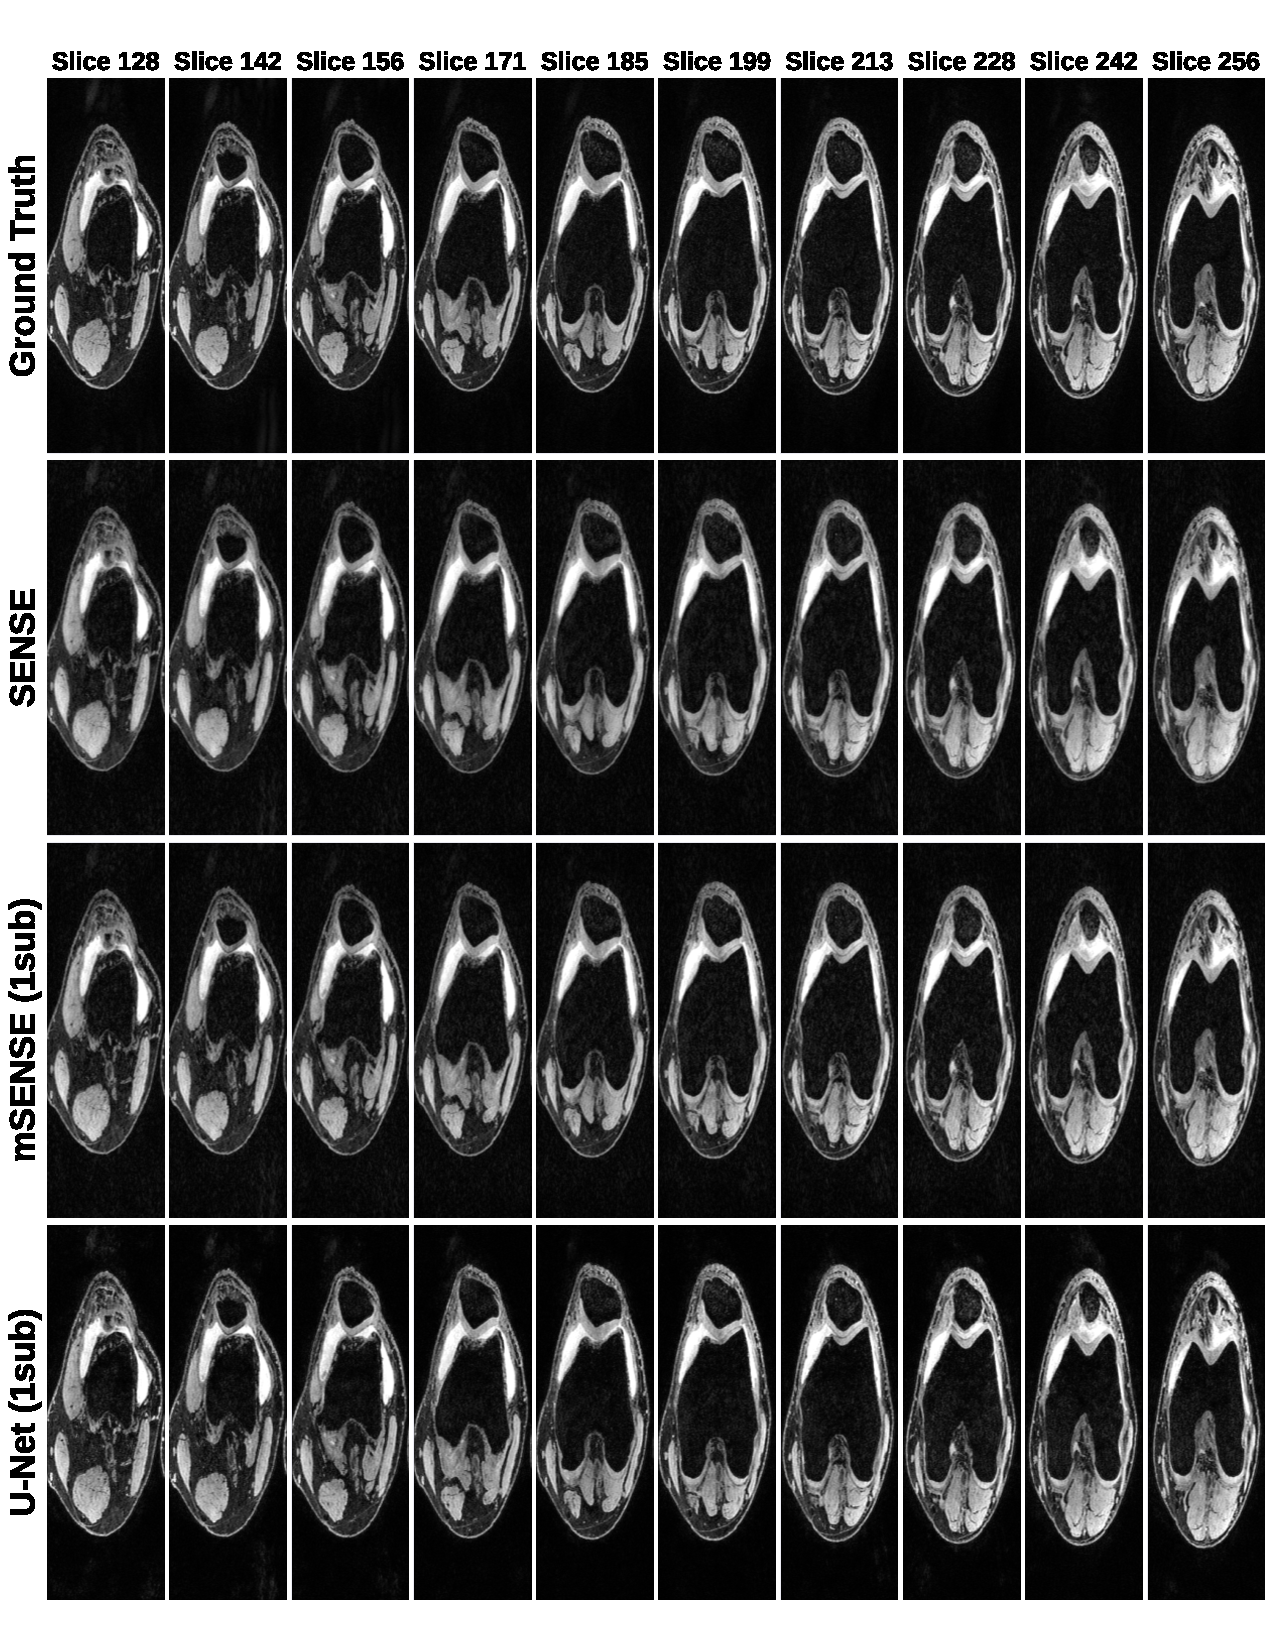
\includegraphics[width=0.9\linewidth]{figures/sample-mri-echo1.pdf}
    \vspace{-1em}
    \caption{Sample reconstructions at 2x acceleration for the first echo in the SKM-TEA dataset using SENSE, Monarch-SENSE (mSENSE), and U-Net. Both mSENSE and U-Net are trained with 1 training scan. SENSE is an untrained method.}
    \label{fig:mri-data-limited-echo1}
\end{figure}

\begin{figure}
    \centering
    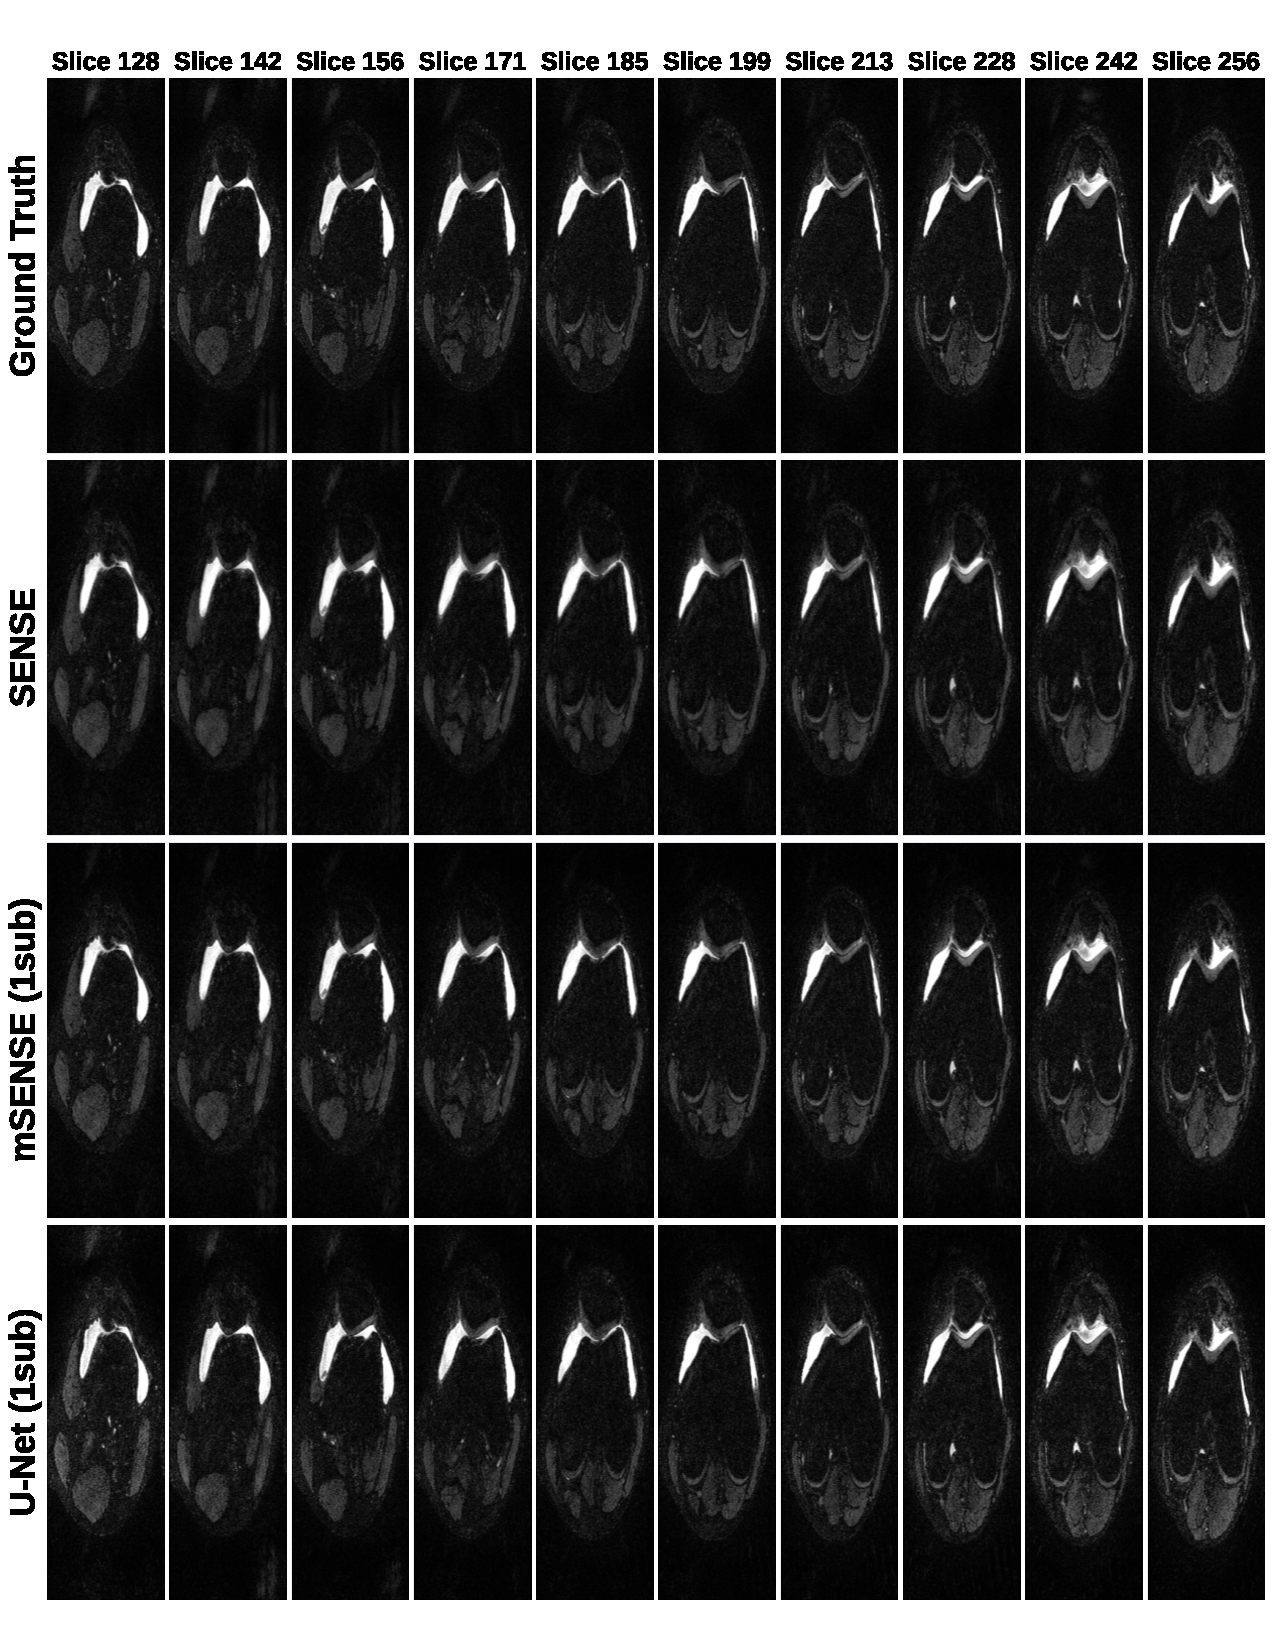
\includegraphics[width=6in]{figures/sample-mri-echo2.pdf}
    \vspace{-1em}
    \caption{Sample reconstructions at 2x acceleration for the second echo in the SKM-TEA dataset using SENSE, Monarch SENSE (mSENSE), and U-Net. Both mSENSE and U-Net are trained with 1 training scan. SENSE is an untrained method.}
    \label{fig:mri-data-limited-echo2}
\end{figure}








\end{document}
